% !TeX program = xelatex
% Conformité guide ENSIASD (template rapport de stage).
% Compilation : xelatex -interaction=nonstopmode main.tex  (deux fois)

\documentclass[12pt,a4paper,oneside]{report}

\usepackage{fontspec}
\usepackage{polyglossia}
\setmainlanguage{french}
\setmainfont{Times New Roman}[
  Ligatures=TeX,
  SmallCapsFont={Times New Roman},
  SmallCapsFeatures={Letters=Uppercase,Scale=0.82}
]

% Guillemets style babel-french (\og \fg), absents de polyglossia.
\providecommand{\og}{\guillemotleft~}
\providecommand{\fg}{\unskip~\guillemotright}

\setlength{\emergencystretch}{3em}
\tolerance=2000

\usepackage[a4paper,top=2.5cm,bottom=2.5cm,left=2.5cm,right=2.5cm,headheight=18pt,headsep=8pt,footskip=22pt]{geometry}
\usepackage{setspace}
\onehalfspacing

\usepackage{amsmath,amssymb}
\usepackage{graphicx}
\usepackage{needspace}
\usepackage{array,booktabs,tabularx,longtable}
\usepackage{xcolor}
\usepackage{colortbl}
\definecolor{ensiBlue}{RGB}{0, 90, 156}
\definecolor{tableHeadBlue}{RGB}{0, 90, 156}
\newcommand{\TableHead}{\rowcolor{tableHeadBlue}}
\newcommand{\tht}[1]{\textcolor{white}{\textbf{#1}}}
% Bloc techno : texte à gauche, logo à droite, espacement élastique
% pour remplir la page sans trou en bas.
\newcommand{\TechBloc}[3]{%
  \par
  \vspace{0.32em plus 0.2em minus 0.08em}%
  {\color{ensiBlue!35}\hrule height 0.45pt}%
  \vspace{0.28em plus 0.12em}%
  \noindent
  \begin{tabular}{@{}p{\dimexpr\textwidth-1.75cm} @{\hspace{0.28cm}} c @{}}
    \textbf{#1.} #3 &
    \raisebox{-0.42\height}{\includegraphics[height=1.05cm]{#2}}
  \end{tabular}%
  \par
}
\usepackage{microtype}
\usepackage{csquotes}
\usepackage{enumitem}
\setlist{nosep,leftmargin=1.5em}

\usepackage[explicit]{titlesec}
\usepackage{fancyhdr}
\usepackage{caption}
\usepackage{tocloft}

% En-tête ENSIASD : libellé italique gras à gauche + filet.
% Chaque style redéfinit entièrement têtes et pieds (fancyhdr).
\newcommand{\EnsiHeadText}{\small\bfseries\itshape\nouppercase{\leftmark}}
\newcommand{\EnsiPageStyle}{%
  \fancyhf{}%
  \renewcommand{\headrulewidth}{0.45pt}%
  \renewcommand{\footrulewidth}{0pt}%
  \fancyhead[L]{\EnsiHeadText}%
  \fancyfoot[R]{\thepage}%
}
\fancypagestyle{plain}{\EnsiPageStyle}
\fancypagestyle{frontmatter}{\EnsiPageStyle}
\fancypagestyle{mainmatter}{\EnsiPageStyle}
\pagestyle{mainmatter}

\renewcommand{\chaptermark}[1]{}
\renewcommand{\sectionmark}[1]{}

\renewcommand{\chaptername}{CHAPITRE}
\newcommand{\EnsiChapterTitle}[1]{%
  \markboth{Chapitre \thechapter{} : #1}{}%
  \MakeUppercase{\chaptername~\thechapter{} : #1}%
}
\newcommand{\EnsiChapterStar}[1]{%
  \markboth{#1}{}%
  \MakeUppercase{#1}%
}
\titleformat{\chapter}[block]
  {\normalfont\bfseries\fontsize{16}{20}\selectfont\raggedleft}
  {}
  {0pt}
  {\EnsiChapterTitle{#1}}
\titlespacing*{\chapter}{0pt}{0pt}{54pt}

\titleformat{name=\chapter,numberless}[block]
  {\normalfont\bfseries\fontsize{16}{20}\selectfont\raggedleft}
  {}
  {0pt}
  {\EnsiChapterStar{#1}}
\titlespacing*{name=\chapter,numberless}{0pt}{0pt}{54pt}

\renewcommand{\thesection}{\Roman{section}}
\titleformat{\section}
  {\normalfont\bfseries\fontsize{14}{18}\selectfont}
  {\thesection.}
  {0.6em}
  {#1}
\titlespacing*{\section}{0pt}{12pt}{12pt}

\renewcommand{\thesubsection}{\thesection.\arabic{subsection}}
\titleformat{\subsection}
  {\normalfont\bfseries\fontsize{12}{16}\selectfont}
  {\thesubsection}
  {0.5em}
  {#1}
\titlespacing*{\subsection}{0pt}{6pt}{6pt}

\renewcommand{\thesubsubsection}{\thesection.\arabic{subsection}.\arabic{subsubsection}}
\titleformat{\subsubsection}
  {\normalfont\bfseries\fontsize{12}{16}\selectfont}
  {\thesubsubsection}
  {0.5em}
  {#1}
\titlespacing*{\subsubsection}{0pt}{6pt}{6pt}

\usepackage{newfloat}
\DeclareFloatingEnvironment[
  fileext=los,
  listname={Liste des schémas},
  name=Schéma,
  placement=htbp
]{schema}

\renewcommand{\thefigure}{\arabic{chapter}.\arabic{figure}}
\renewcommand{\thetable}{\arabic{chapter}.\arabic{table}}
\renewcommand{\theschema}{\arabic{chapter}.\arabic{schema}}

\DeclareCaptionLabelFormat{ensi}{#1 : #2}
\captionsetup[figure]{
  name={Figure},
  font={it},
  justification=centering,
  skip=6pt,
  labelformat=ensi,
  labelsep=colon
}
\captionsetup[schema]{
  font={it},
  justification=centering,
  skip=6pt,
  labelformat=ensi,
  labelsep=colon
}
% Tableaux : titre en haut, 11 pt, centré
\captionsetup[table]{
  font={it},
  justification=centering,
  skip=6pt,
  labelformat=ensi,
  labelsep=colon,
  position=top
}
\usepackage{etoolbox}
\AtBeginEnvironment{figure}{\fontsize{11}{13}\selectfont}
\AtBeginEnvironment{table}{\fontsize{11}{13}\selectfont}
\AtBeginEnvironment{schema}{\fontsize{11}{13}\selectfont}
\AfterEndPreamble{%
  \renewcommand{\figurename}{Figure}%
  \renewcommand{\tablename}{Tableau}%
}

\graphicspath{{figures/}{../rapport/}}

\newcommand{\FigPlaceholder}[1]{%
  \begin{center}
    \fbox{\parbox{0.88\textwidth}{\centering\vspace{2.2cm}\textit{#1}\vspace{2.2cm}}}
  \end{center}
}

\setcounter{tocdepth}{3}
\setcounter{secnumdepth}{3}

\setlength{\parindent}{1.25em}
\setlength{\parskip}{0pt}

\usepackage{xurl}
\usepackage{hyperref}
\usepackage{bookmark}

\AtBeginDocument{%
  \renewcommand{\contentsname}{Table des matières}%
  \renewcommand{\listfigurename}{Liste des figures}%
  \renewcommand{\listtablename}{Liste des tableaux}%
  \renewcommand{\bibname}{Références bibliographiques}%
  \renewcommand{\figurename}{Figure}%
  \renewcommand{\tablename}{Tableau}%
}

\makeatletter
\renewcommand\tableofcontents{%
  \chapter*{\contentsname}%
  \@starttoc{toc}%
}
\renewcommand\listoffigures{%
  \chapter*{\listfigurename}%
  \@starttoc{lof}%
}
\renewcommand\listoftables{%
  \chapter*{\listtablename}%
  \@starttoc{lot}%
}
\makeatother

% Compléter les champs entre crochets avant impression.
\newcommand{\NomAuteur}{Hamza Bendaib}
\newcommand{\Filiere}{Ingénierie Logicielle}
% Autres filières ENSIASD : Sciences des Données, Big Data \& IA ;
% Sécurité IT et Confiance Numérique ; Management et Gouvernance des SI.
\newcommand{\ThemeStage}{SmartTrans-AI : plateforme de gestion de transport enrichie par l'intelligence artificielle}
\newcommand{\DateSoutenance}{}
\newcommand{\HeureSoutenance}{}
\newcommand{\AnneeUniv}{2025--2026}
\newcommand{\PresidentJury}{[Pr. Nom]}
\newcommand{\ExaminateurA}{[Pr. Nom]}
\newcommand{\ExaminateurB}{[Pr. Nom]}
\newcommand{\EncadrantEcole}{Mme Loubna Karbil}
\newcommand{\EncadrantEntreprise}{Mme Sara Zaqi}
\newcommand{\EtablissementAccueil}{S. WATRANS}
\newcommand{\LieuSoutenance}{ENSIASD de Taroudant}


\hypersetup{
  colorlinks=true,
  linkcolor=black,
  citecolor=black,
  urlcolor=black,
  pdftitle={Rapport de stage --- SmartTrans-AI},
  pdfauthor={\NomAuteur}
}

\begin{document}

% Couverture : aucun numéro.
\pagestyle{empty}
\pagenumbering{gobble}
\begin{titlepage}
\thispagestyle{empty}
\setstretch{1.05}
\centering

\vspace*{-1.85cm}

\includegraphics[width=0.98\textwidth]{ensi-en-tete.png}\\[0.12cm]
{\color{ensiBlue}\rule{\textwidth}{6pt}}

\vspace{0.7cm}

{\fontsize{16}{19}\selectfont\bfseries RAPPORT DE STAGE D'INITIATION}

\vspace{0.35cm}

{\fontsize{12}{14}\selectfont
Filière : « Ingénierie Logicielle »
}

\vspace{0.45cm}

{\color{ensiBlue}\rule{0.92\textwidth}{1.4pt}}\\[0.28cm]
{\fontsize{18}{21}\selectfont\bfseries SMARTTRANS-AI}\\[0.12cm]
{\fontsize{12}{15}\selectfont\bfseries
Plateforme de gestion de transport enrichie par l'intelligence artificielle
}\\[0.28cm]
{\color{ensiBlue}\rule{0.92\textwidth}{1.4pt}}

\vspace{0.5cm}

{\fontsize{12}{14}\selectfont
Présenté par\\[0.22cm]
\textbf{\NomAuteur}
}

\vspace{0.4cm}

{\fontsize{12}{14}\selectfont
Soutenue le \underline{\hspace{3.6cm}} à \underline{\hspace{2.4cm}}
}

\vfill

{\fontsize{12}{14}\selectfont\bfseries Devant le jury}\\[0.35cm]
\renewcommand{\arraystretch}{1.45}
\fontsize{11}{13}\selectfont
\begin{tabular}{lll}
Pr  & \underline{\hspace{3.6cm}}, professeur à l'ENSIASD de Taroudant & Président \\
Pr  & \underline{\hspace{3.6cm}}, professeur à l'ENSIASD de Taroudant & Examinateur \\
Pr  & \underline{\hspace{3.6cm}}, professeur à l'ENSIASD de Taroudant & Examinateur \\
Mme & Loubna Karbil, professeure à l'ENSIASD de Taroudant & Encadrante pédagogique \\
Mme & Sara Zaqi, établissement d'accueil : S. WATRANS & Encadrante \\
\end{tabular}

\vspace{1.1cm}

{\fontsize{12}{14}\selectfont
Année universitaire \AnneeUniv
}

\vfill

{\color{ensiBlue}\rule{\textwidth}{6pt}}
\vspace*{-1.05cm}
\end{titlepage}


% Comptage à partir de la 2e page, chiffres arabes.
\clearpage
\pagenumbering{arabic}
\pagestyle{mainmatter}

\chapter*{Dédicaces}

Je dédie ce travail à ma famille, pour son amour, son soutien constant et ses encouragements qui m'ont accompagné tout au long de mon parcours académique. Votre présence et votre confiance ont été une source de motivation et de persévérance dans les moments les plus difficiles.

À mes enseignants de l'ENSIASD de Taroudant, pour leur engagement, leur patience et les connaissances qu'ils m'ont transmises, notamment dans les domaines de l'informatique, de l'ingénierie logicielle et de l'intelligence artificielle. Leur enseignement a contribué à construire les bases qui m'ont permis de mener à bien ce projet.

À mes encadrants de stage, pour leur confiance, leurs conseils et leur accompagnement durant la conception et la réalisation de SmartTrans-AI. Leurs orientations et leurs remarques m'ont permis d'enrichir mes connaissances et de développer davantage mes compétences professionnelles.

Enfin, je dédie ce travail à toutes les personnes qui, de près ou de loin, m'ont encouragé et soutenu tout au long de cette expérience.

\clearpage
\chapter*{Remerciements}

Je tiens à remercier en premier lieu mon encadrante pédagogique, \textbf{Mme Loubna Karbil}, pour son suivi tout au long de ce stage, ses conseils, sa disponibilité et ses orientations méthodologiques. Son accompagnement m'a permis de mieux structurer mon travail, d'approfondir ma réflexion et de mener à bien les différentes étapes de ce projet.

Mes sincères remerciements s'adressent également à mon encadrante au sein de \textbf{S. WATRANS}, \textbf{Mme Sara Zaqi}, pour m'avoir accueilli au sein de l'entreprise et plus particulièrement au sein du département informatique. Je la remercie pour la confiance qu'elle m'a accordée en me confiant le projet \textbf{SmartTrans-AI}, ainsi que pour sa disponibilité, ses conseils et les échanges qui m'ont permis de mieux comprendre les besoins et les problématiques liés au domaine du transport et de la gestion de flotte.

Je souhaite également exprimer ma gratitude à l'ensemble des collaborateurs de \textbf{S. WATRANS} pour leur accueil, leur disponibilité et leur bienveillance durant toute la période de mon stage. Leur collaboration et leurs explications m'ont permis de découvrir davantage le fonctionnement d'une entreprise et de mieux comprendre l'importance des outils informatiques dans la gestion quotidienne de ses activités.

Ce stage a constitué pour moi une expérience particulièrement enrichissante, aussi bien sur le plan technique que professionnel. Il m'a permis de mettre en pratique les connaissances acquises durant ma formation, notamment dans les domaines du développement logiciel, des bases de données, de la conception des systèmes et de l'intelligence artificielle. Il m'a également permis de développer mon autonomie, mon esprit d'analyse, ma capacité à résoudre des problèmes et mon aptitude à travailler sur un projet répondant à des besoins réels.

Je remercie également l'ensemble du corps professoral de l'\textbf{ENSIASD de Taroudant} pour la qualité de l'enseignement dispensé et pour les connaissances et compétences acquises au cours de ma formation. Ces acquis ont constitué une base importante pour la réalisation de ce stage et du projet qui m'a été confié.

Je tiens aussi à remercier mes camarades de promotion pour leur soutien, leurs échanges d'idées et les discussions techniques qui ont contribué à rendre cette expérience plus enrichissante.

Enfin, j'adresse mes plus sincères remerciements à ma famille pour son soutien constant, ses encouragements, sa patience et sa confiance. Leur accompagnement m'a donné la motivation nécessaire pour avancer et donner le meilleur de moi-même tout au long de cette période.

À toutes les personnes qui ont contribué, directement ou indirectement, à la réussite de ce stage et à la réalisation de ce projet, je leur adresse mes sincères remerciements et ma profonde gratitude.

\clearpage
\chapter*{Résumé}

Ce rapport présente le projet de stage \textbf{SmartTrans-AI}, plateforme de gestion de transport enrichie par l'intelligence artificielle. L'application permet de planifier et de suivre des missions, de gérer les clients, les chauffeurs et les véhicules, et d'alerter sur les échéances critiques (permis de conduire, assurance, visite technique). Trois profils sont distingués : administrateur, responsable transport et chauffeur. L'authentification repose sur JSON Web Token (JWT) et des rôles. Un journal d'activités, en lecture seule, trace automatiquement les opérations. Un assistant conversationnel, ancré sur les données métier, répond aux questions opérationnelles et propose des ressources disponibles. La réalisation s'appuie sur Spring Boot (API REST), PostgreSQL, React et Vite. Ce document décrit le cadre du stage, l'analyse et la conception (cas d'utilisation, classes), la réalisation, les tests et les perspectives.

\vspace{0.8em}
\noindent\textbf{Mots-clés :} gestion de transport, missions, JWT, Spring Boot, React, assistant IA, audit.

\clearpage
\chapter*{Abstract}

This internship report presents the \textbf{SmartTrans-AI} project, a transport management platform enhanced with artificial intelligence. The application supports the planning and tracking of missions, the management of clients, drivers and vehicles, and alerts on critical expiry dates (driving licence, insurance, technical inspection). Three user profiles are distinguished: administrator, transport manager and driver. Authentication is based on JSON Web Token (JWT) and roles. A read-only activity log automatically records operations. A conversational assistant, grounded in business data, answers operational questions and suggests available resources. The implementation relies on Spring Boot (REST API), PostgreSQL, React and Vite. This document describes the internship context, the analysis and design (use cases, class diagram), the implementation, the tests and the outlook.

\vspace{0.8em}
\noindent\textbf{Keywords:} transport management, missions, JWT, Spring Boot, React, AI assistant, audit.


\clearpage
\tableofcontents

\clearpage
\chapter*{Liste des abréviations}
\addcontentsline{toc}{chapter}{Liste des abréviations}
\begin{flushleft}
\renewcommand{\arraystretch}{1.25}
\begin{tabular}{@{}p{0.28\textwidth}p{0.68\textwidth}@{}}
\textbf{API} & Application Programming Interface \\
\textbf{CORS} & Cross-Origin Resource Sharing \\
\textbf{CRUD} & Create, Read, Update, Delete \\
\textbf{CT} & Contrôle technique (visite technique) \\
\textbf{ENSIASD} & École Nationale Supérieure d'Intelligence Artificielle et Sciences des Données de Taroudant \\
\textbf{HTTP} & HyperText Transfer Protocol \\
\textbf{IA} & Intelligence artificielle \\
\textbf{JPA} & Jakarta Persistence API \\
\textbf{JSON} & JavaScript Object Notation \\
\textbf{JWT} & JSON Web Token \\
\textbf{KPI} & Key Performance Indicator \\
\textbf{LLM} & Large Language Model \\
\textbf{REST} & Representational State Transfer \\
\textbf{SI} & Système d'information \\
\textbf{UML} & Unified Modeling Language \\
\textbf{UUID} & Universally Unique Identifier \\
\end{tabular}
\end{flushleft}


\clearpage
\addcontentsline{toc}{chapter}{Liste des figures}
\listoffigures

\clearpage
\addcontentsline{toc}{chapter}{Liste des tableaux}
\listoftables

\clearpage
\addcontentsline{toc}{chapter}{Liste des schémas}
\listofschemas

\clearpage
\pagestyle{mainmatter}

\chapter*{Introduction générale}
\addcontentsline{toc}{chapter}{Introduction générale}

Le secteur du transport routier de marchandises repose sur une coordination permanente entre clients, chauffeurs, véhicules et missions. Une organisation qui s'appuie uniquement sur des tableurs ou des échanges informels expose l'exploitant à des oublis : mission mal affectée, véhicule indisponible, permis ou assurance arrivés à échéance. Ces ruptures ont un coût opérationnel et réglementaire.

Le projet de stage \textbf{SmartTrans-AI} vise à concevoir et réaliser une application web de gestion de transport, enrichie par un assistant conversationnel. L'objectif n'est pas de remplacer le responsable d'exploitation, mais de centraliser les données, de tracer les actions et d'accélérer les recherches du type : combien de missions sont en cours, quel chauffeur est disponible, quel véhicule peut être affecté.

Le périmètre retenu comprend l'authentification, le tableau de bord, la gestion des utilisateurs (administrateur), des clients, des chauffeurs et des véhicules, le cycle de vie des missions, le journal d'activités, les alertes d'expiration et l'assistant IA. Sont volontairement exclus du produit livré un module documentaire de type GED et un écran de notifications push. Le chauffeur peut consulter ses missions, les démarrer et les terminer ; il ne peut pas les annuler.

Ce rapport s'organise en sept chapitres. Le premier situe le cadre du stage chez S. WATRANS. Le deuxième dresse un état de l'art et positionne le produit. Le troisième présente l'analyse et la conception (cas d'utilisation, classes, données). Le quatrième décrit la réalisation. Le cinquième traite des tests, du déploiement et des limites. Le sixième revient sur la conduite de projet. Le septième présente les interfaces (captures d'écran). Une conclusion générale ouvre des perspectives.


\chapter{Cadre du stage et étude préalable}

\section{Introduction}

Ce chapitre précise le contexte du stage, les missions confiées, les acteurs métier et les choix technologiques qui ont orienté la réalisation de SmartTrans-AI.

\section{Organisme d'accueil et missions du stagiaire}

\subsection{Présentation de l'organisme}

\begin{center}

\includegraphics[width=4.8cm]{logo-swatrans.png}
\end{center}

S. WATRANS est une société spécialisée dans le transport de marchandises, la vente et l'achat de matériaux de construction, ainsi que dans la réalisation de travaux divers et de construction. Grâce à la diversité de ses activités, l'entreprise assure différents services liés au transport, à la logistique et au secteur du bâtiment.

Afin d'accompagner et de faciliter la gestion de ses différentes activités, la société dispose également d'un département informatique, chargé de la gestion et du développement des solutions informatiques utilisées au sein de l'entreprise. C'est au sein de ce département que j'ai effectué mon stage, en participant aux activités et aux travaux liés au développement et à l'amélioration des solutions informatiques de l'entreprise.

\subsection{Missions confiées et planning}

Les travaux confiés au stagiaire, au sein du département informatique, ont porté sur la spécification des rôles, la conception du modèle de données, le développement de l'API REST, l'interface React, l'assistant ancré sur les données, et la rédaction de ce rapport. Le découpage temporel et les risques sont détaillés au chapitre consacré à la conduite de projet.

\section{Problématique et besoins métier}

\subsection{Problématique}

Sans système partagé, le responsable transport ne dispose pas d'une vision fiable des missions (planifiées, en cours, terminées, annulées) ni d'alertes sur les documents arrivant à expiration. Le chauffeur, de son côté, a besoin d'un accès simple à «~ses~» missions, sans droits de planification.

\subsection{Besoins fonctionnels}

Les besoins fonctionnels principaux sont : s'authentifier ; consulter un tableau de bord ; gérer les clients, chauffeurs, véhicules et missions ; consulter un journal d'audit ; interroger un assistant ; pour le chauffeur, suivre et clôturer ses courses.

\subsection{Besoins non fonctionnels}

L'application doit être utilisable via un navigateur, reposer sur une API documentée, séparer les droits selon le rôle, et rester déployable localement (développement) ou via des conteneurs. La confidentialité des mots de passe impose un hachage côté serveur. L'assistant ne doit pas inventer des missions absentes de la base : les réponses s'appuient sur un contexte métier extrait de PostgreSQL.

\section{Acteurs}

Trois acteurs correspondent aux codes de rôle \texttt{ADMIN}, \texttt{TRANSPORT\_MANAGER} et \texttt{DRIVER} (tableau~\ref{tab:acteurs}).

\begin{table}[htbp]
\centering
\caption{Acteurs et périmètre fonctionnel}
\label{tab:acteurs}
\begin{tabular}{|p{0.28\textwidth}|p{0.62\textwidth}|}
\hline
\TableHead
\tht{Acteur} & \tht{Périmètre} \\
\hline
Administrateur & Utilisateurs et rôles, tout le métier, journal, assistant, tableau de bord \\
\hline
Responsable transport & Métier, journal, assistant, tableau de bord ; pas de gestion des comptes utilisateurs \\
\hline
Chauffeur & Tableau de bord, ses missions, démarrage et fin de mission, profil, alertes permis \\
\hline
\end{tabular}
\end{table}

\section{Choix technologiques}

L'architecture retenue est une application web à deux volets : une API REST côté serveur et une interface web côté client. Chaque composant de la stack a un rôle précis, rappelé ci-dessous, avec son logo à droite.

\TechBloc{Java}{logos/java.png}{%
Java est le socle du backend : typage statique et code structuré, testable pendant le stage.}

\TechBloc{Spring Boot}{logos/spring.png}{%
Spring Boot orchestre l'API REST (\texttt{/api/v1}), JPA, la sécurité et les tests \cite{spring}.}

\TechBloc{PostgreSQL}{logos/postgresql.png}{%
PostgreSQL stocke utilisateurs, clients, chauffeurs, véhicules, missions et journal \cite{postgres}.}

\TechBloc{JWT}{logos/jwt.png}{%
Après le login, le client envoie un JSON Web Token \cite{jwt} dans \texttt{Authorization}. L'API reste sans état.}

\TechBloc{React}{logos/react.png}{%
React construit l'interface (tableau de bord, formulaires, vues selon le profil) \cite{react}.}

\TechBloc{TypeScript}{logos/typescript.png}{%
TypeScript type le client et limite les écarts de contrat avec l'API (identifiants, statuts, rôles).}

\TechBloc{Vite}{logos/vite.png}{%
Vite compile le front. Un proxy vers le port 8080 évite les blocages CORS en développement.}

\TechBloc{Flyway}{logos/flyway.png}{%
Flyway versionne le schéma : les migrations alignent la base sur le code, en local comme en conteneur.}

\TechBloc{OpenAI}{logos/openai.png}{%
Avec \texttt{OPENAI\_API\_KEY}, l'assistant appelle Chat Completions (\texttt{gpt-4o-mini}). Sinon, le mode \texttt{GROUNDED} s'appuie sur les données locales.}

\section{Conclusion}

Le cadre du stage fixe un produit de transport, trois rôles et une architecture API plus interface. Le chapitre suivant situe ce choix face à l'état de l'art.

\chapter{État de l'art et positionnement}

\section{Introduction}

Avant de spécifier SmartTrans-AI, il convient de situer le projet dans le paysage des systèmes de gestion de transport (TMS), des pratiques d'exploitation encore largement manuelles, et des usages émergents de l'intelligence artificielle en logistique. Ce chapitre justifie le positionnement du livrable : un outil métier ciblé, sécurisé, et un assistant ancré sur les données de l'entreprise plutôt qu'un TMS générique du marché.

\section{Gestion de transport et systèmes d'information}

\subsection{Le métier de TMS}

Un \textit{Transport Management System} vise à planifier les tournées, affecter les ressources (chauffeurs, véhicules), suivre l'exécution et produire des indicateurs. Les éditeurs internationaux proposent des suites souvent coûteuses, longues à paramétrer, et parfois surdimensionnées pour une PME de transport et de BTP telle que S. WATRANS. À l'opposé, de nombreuses exploitations s'appuient encore sur des tableurs, la messagerie et le téléphone. Ces outils restent souples, mais ils ne garantissent ni l'unicité de l'information, ni la traçabilité, ni le contrôle d'accès par rôle.

\subsection{Limites des pratiques non intégrées}

Lorsque les missions sont saisies dans un fichier partagé, les risques sont connus : versions divergentes, absence d'historique fiable, difficulté à savoir si un chauffeur est déjà en course, oubli des dates de permis ou d'assurance. Le besoin exprimé pendant le stage n'était pas de reproduire toute la richesse d'un TMS du marché, mais de couvrir un noyau : clients, flotte, missions, alertes, journal, et un canal de questionnement rapide (assistant).

\section{Authentification, API et applications web}

Les applications d'entreprise actuelles séparent souvent une interface web d'une API REST. L'authentification par session serveur reste possible ; le jeton JWT, largement documenté \cite{jwt}, permet à l'interface de rester sans état côté API, ce qui simplifie le déploiement et le passage à l'échelle. Spring Security et Spring Boot offrent un cadre éprouvé pour exposer des ressources protégées par rôle \cite{spring}. Côté client, React s'est imposé pour des interfaces modulaires \cite{react}. PostgreSQL reste un choix robuste pour un modèle relationnel métier \cite{postgres}.

Le tableau~\ref{tab:comparaison-stack} résume les alternatives envisagées et le choix retenu.

\begin{table}[htbp]
\centering
\caption{Positionnement des choix techniques}
\label{tab:comparaison-stack}
\begin{tabular}{|p{0.22\textwidth}|p{0.32\textwidth}|p{0.36\textwidth}|}
\hline
\TableHead
\tht{Composant} & \tht{Alternatives} & \tht{Choix et motif} \\
\hline
Backend & Node.js, Django, .NET & Spring Boot : typage Java, sécurité, JPA, tests d'intégration \\
\hline
Frontend & Angular, Vue & React + Vite : écosystème, rapidité de développement \\
\hline
Base de données & MySQL, MongoDB & PostgreSQL : relations, contraintes, JSON pour l'audit \\
\hline
Auth & Session, OAuth2 complet & JWT : API stateless, rôles, simplicité de mise en œuvre \\
\hline
IA & Chat générique sans contexte & Assistant ancré sur missions, chauffeurs, véhicules, clients \\
\hline
\end{tabular}
\end{table}

\section{Intelligence artificielle en exploitation}

Les modèles de langage permettent de formuler des questions en langue naturelle. Sans ancrage, ils hallucinent des effectifs ou des immatriculations. La littérature et les retours d'usage insistent sur la \textit{grounding} : fournir un contexte issu du SI. SmartTrans-AI adopte cette approche : extraction d'un résumé opérationnel, puis génération éventuelle via une clé d'API, ou réponses déterministes si la clé est absente. L'IA n'est pas un module de planification automatique des tournées (problème d'optimisation combinatoire) ; elle assiste la consultation et la suggestion de ressources disponibles.

\section{Positionnement de SmartTrans-AI}

SmartTrans-AI se situe entre le tableur et le TMS complet. Il est spécifique au besoin du département informatique de S. WATRANS : digitaliser le suivi des missions et de la conformité minimale de la flotte, avec trois profils, un audit automatique et un assistant. Les fonctionnalités de GED et de notifications temps réel ont été écartées pour tenir le calendrier du stage et rester sur un produit démontrable.

\section{Conclusion}

L'état de l'art confirme l'intérêt d'une application web sécurisée, d'un modèle relationnel clair, et d'une IA contrainte par les données. Le chapitre suivant traduit ces orientations en cas d'utilisation et en conception UML.

\chapter{Analyse et conception}

\section{Introduction}

Ce chapitre formalise le système : cas d'utilisation, scénarios dynamiques (dont le diagramme de séquence de l'assistant), diagramme de classes du domaine, schéma relationnel et architecture de déploiement. Les diagrammes UML suivent le guide ENSIASD pour la numérotation des figures \cite{uml}.

\section{Cas d'utilisation}

\subsection{Présentation du diagramme}

Le diagramme de cas d'utilisation (figure~\ref{fig:cu}) regroupe les fonctions autour de quatre paquets : commun, métier, administration et espace chauffeur. Tous les acteurs s'authentifient par JWT. L'administrateur et le responsable partagent la gestion des clients, chauffeurs, véhicules et missions, ainsi que le journal et l'assistant. Seul l'administrateur gère les utilisateurs et les rôles. Le chauffeur consulte ses missions, change le statut (démarrer / terminer) et met à jour son profil.

\begin{figure}[htbp]
\centering
\IfFileExists{figures/diagramme-cas-utilisation.png}{%
  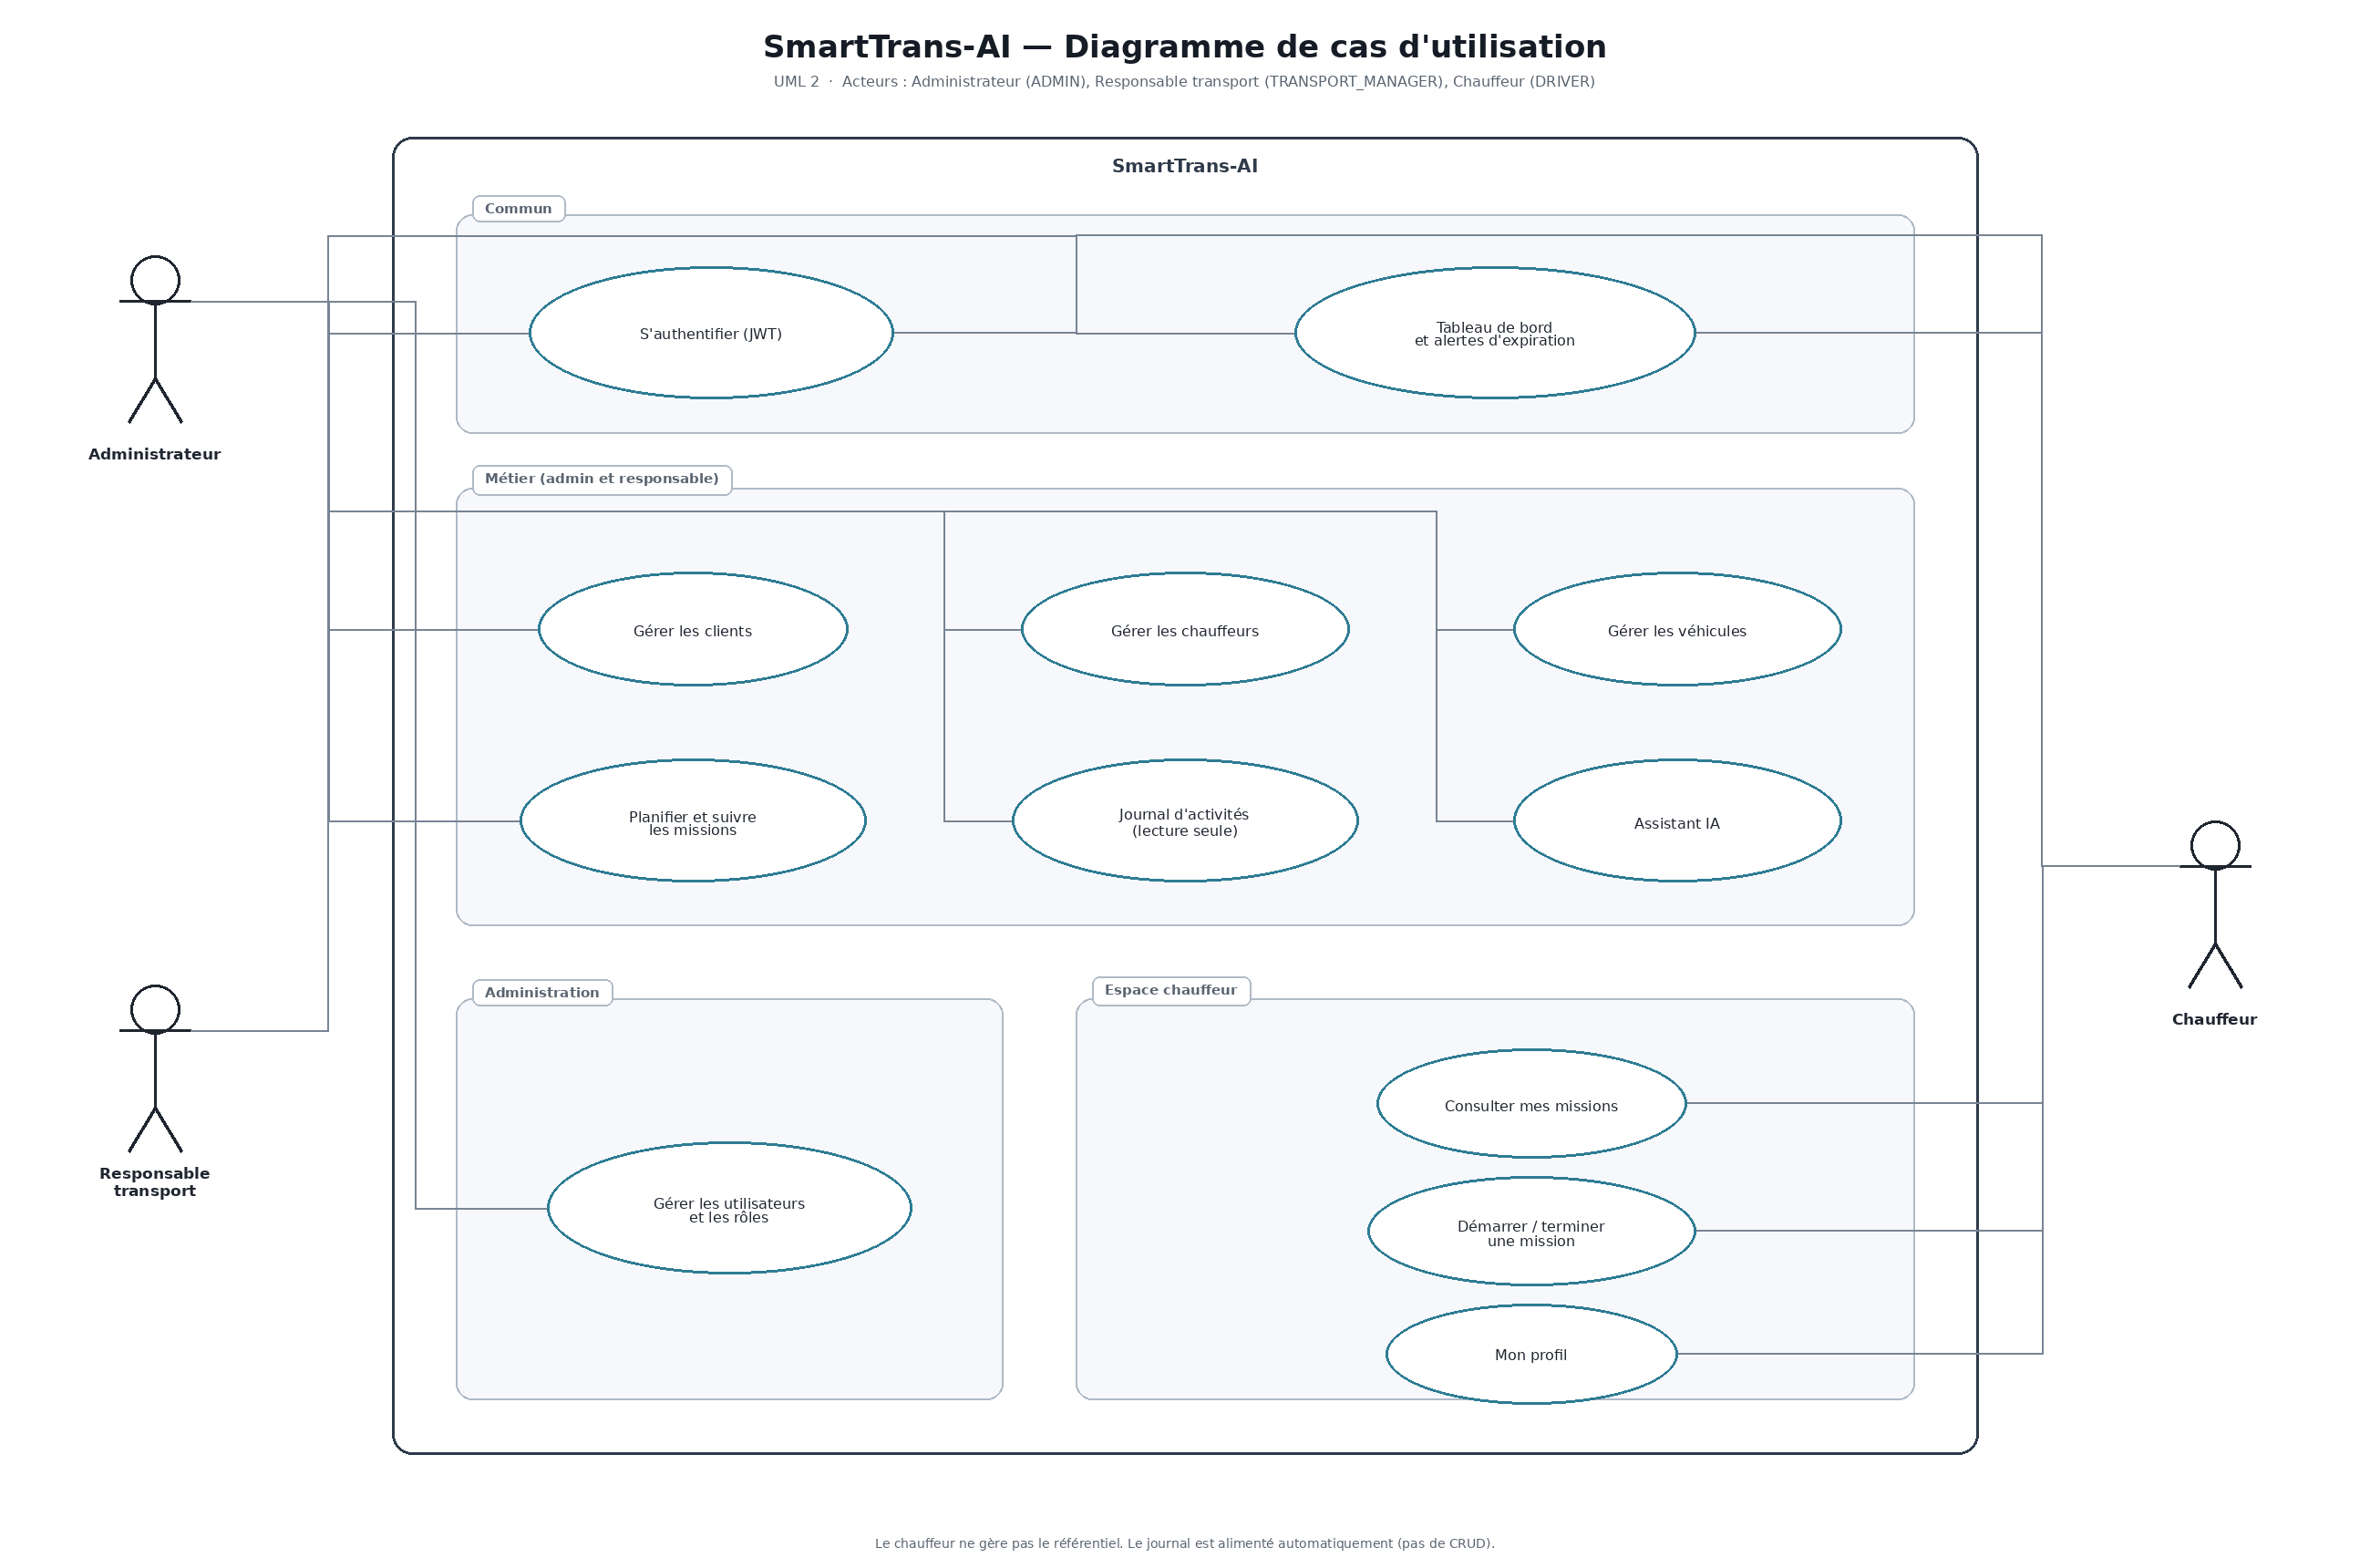
\includegraphics[width=\textwidth,keepaspectratio]{diagramme-cas-utilisation.png}%
}{%
  \FigPlaceholder{Générer \texttt{docs/soutenance/draw\_cas\_utilisation.py}\\vers \texttt{docs/rapport-stage/figures/diagramme-cas-utilisation.png}}%
}
\caption{Diagramme de cas d'utilisation de SmartTrans-AI}
\label{fig:cu}
\end{figure}

\subsection{Description des cas principaux}

L'authentification délivre un jeton utilisé sur les routes protégées. Le tableau de bord agrège des indicateurs (volumes de missions, graphiques, rappels d'expiration). La planification d'une mission associe un client obligatoire, un chauffeur et un véhicule optionnels, un trajet, une date et un statut (\texttt{PLANIFIED}, \texttt{IN\_PROGRESS}, \texttt{COMPLETED}, \texttt{CANCELLED}). Le journal est alimenté automatiquement (créations, mises à jour, suppressions, changements de statut, connexions) et n'offre pas de CRUD manuel. L'assistant répond à des questions du type effectifs de missions ou suggestions de chauffeur et de véhicule disponibles.

\subsection{Fiches de cas d'utilisation}

Les tableaux~\ref{tab:cu-auth} à~\ref{tab:cu-chauffeur} décrivent les cas les plus structurants, au format habituel (acteur, préconditions, enchaînement, exceptions).

\begin{table}[htbp]
\centering
\caption{Cas d'utilisation : s'authentifier}
\label{tab:cu-auth}
\begin{tabular}{|p{0.28\textwidth}|p{0.62\textwidth}|}
\hline
\TableHead
\tht{Identifiant} & \textcolor{white}{CU-AUTH} \\
\hline
Acteurs & Administrateur, responsable transport, chauffeur \\
\hline
Précondition & Compte existant, activé \\
\hline
Enchaînement & Saisie courriel et mot de passe ; vérification du hachage ; émission d'un JWT ; redirection vers le tableau de bord \\
\hline
Exceptions & Identifiants invalides, compte désactivé, origine CORS refusée \\
\hline
Postcondition & Le client conserve le jeton pour les appels suivants \\
\hline
\end{tabular}
\end{table}

\begin{table}[htbp]
\centering
\caption{Cas d'utilisation : planifier et suivre une mission}
\label{tab:cu-mission}
\begin{tabular}{|p{0.28\textwidth}|p{0.62\textwidth}|}
\hline
\TableHead
\tht{Identifiant} & \textcolor{white}{CU-MIS} \\
\hline
Acteurs & Administrateur, responsable transport (écriture) ; chauffeur (statut de ses missions) \\
\hline
Précondition & Client existant ; éventuellement chauffeur et véhicule disponibles \\
\hline
Enchaînement & Création (référence, trajet, date) ; affectation ; passage planifiée $\rightarrow$ en cours $\rightarrow$ terminée ; consultation des listes et filtres \\
\hline
Exceptions & Référence déjà utilisée ; chauffeur non affecté qui tente un changement de statut ; tentative d'annulation par le chauffeur \\
\hline
Postcondition & Mission persistée ; événement d'audit enregistré \\
\hline
\end{tabular}
\end{table}

\begin{table}[htbp]
\centering
\caption{Cas d'utilisation : espace chauffeur}
\label{tab:cu-chauffeur}
\begin{tabular}{|p{0.28\textwidth}|p{0.62\textwidth}|}
\hline
\TableHead
\tht{Identifiant} & \textcolor{white}{CU-DRV} \\
\hline
Acteur & Chauffeur \\
\hline
Précondition & Compte lié à une fiche chauffeur \\
\hline
Enchaînement & Consultation de mes missions ; démarrage ; clôture ; mise à jour du profil et de la disponibilité \\
\hline
Exceptions & Mission non affectée ; statut métier incompatible \\
\hline
\end{tabular}
\end{table}

\section{Scénarios dynamiques}

\subsection{Authentification}

Le navigateur envoie les identifiants à \texttt{POST /api/v1/auth/login} sans en-tête Bearer. L'API valide les informations, construit le jeton et renvoie le profil (rôles). Les appels suivants portent \texttt{Authorization: Bearer}. Un filtre ignore les routes d'authentification afin d'éviter un 403 sur le login.

\subsection{Cycle de vie d'une mission}

Le responsable crée la mission (statut planifiée). Le chauffeur authentifié appelle le changement de statut. Le serveur vérifie l'affectation et la transition autorisée, met à jour les horodatages \texttt{startedAt} / \texttt{completedAt}, et journalise l'action. L'annulation n'est pas exposée au profil chauffeur.

\subsection{Question à l'assistant}

L'administrateur ou le responsable transport saisit une question depuis l'interface. Le diagramme de séquence de la figure~\ref{fig:seq-assistant} détaille les échanges. Le navigateur envoie \texttt{POST /api/v1/assistant/ask} avec l'en-tête \texttt{Authorization: Bearer}. Le filtre JWT vérifie la signature et l'expiration du jeton. S'il est absent, invalide ou expiré, l'API répond \texttt{401} et l'utilisateur revient à l'écran de connexion, sans lecture des données.

Lorsque le jeton est valide, \texttt{AssistantService} interroge PostgreSQL et constitue un contexte ancré (missions, chauffeurs, véhicules, clients). Si une clé d'API est configurée, ce contexte est transmis à OpenAI (\texttt{POST /chat/completions}) et la réponse porte le mode \texttt{LLM}. Sinon, ou si l'appel échoue, le service compose lui-même une réponse courte, par exemple un effectif de missions (mode \texttt{GROUNDED}). Dans les deux cas, le client reçoit le texte, le mode et les citations, puis les affiche.

\begin{figure}[htbp]
\centering
\IfFileExists{figures/diagramme-sequence.png}{%
  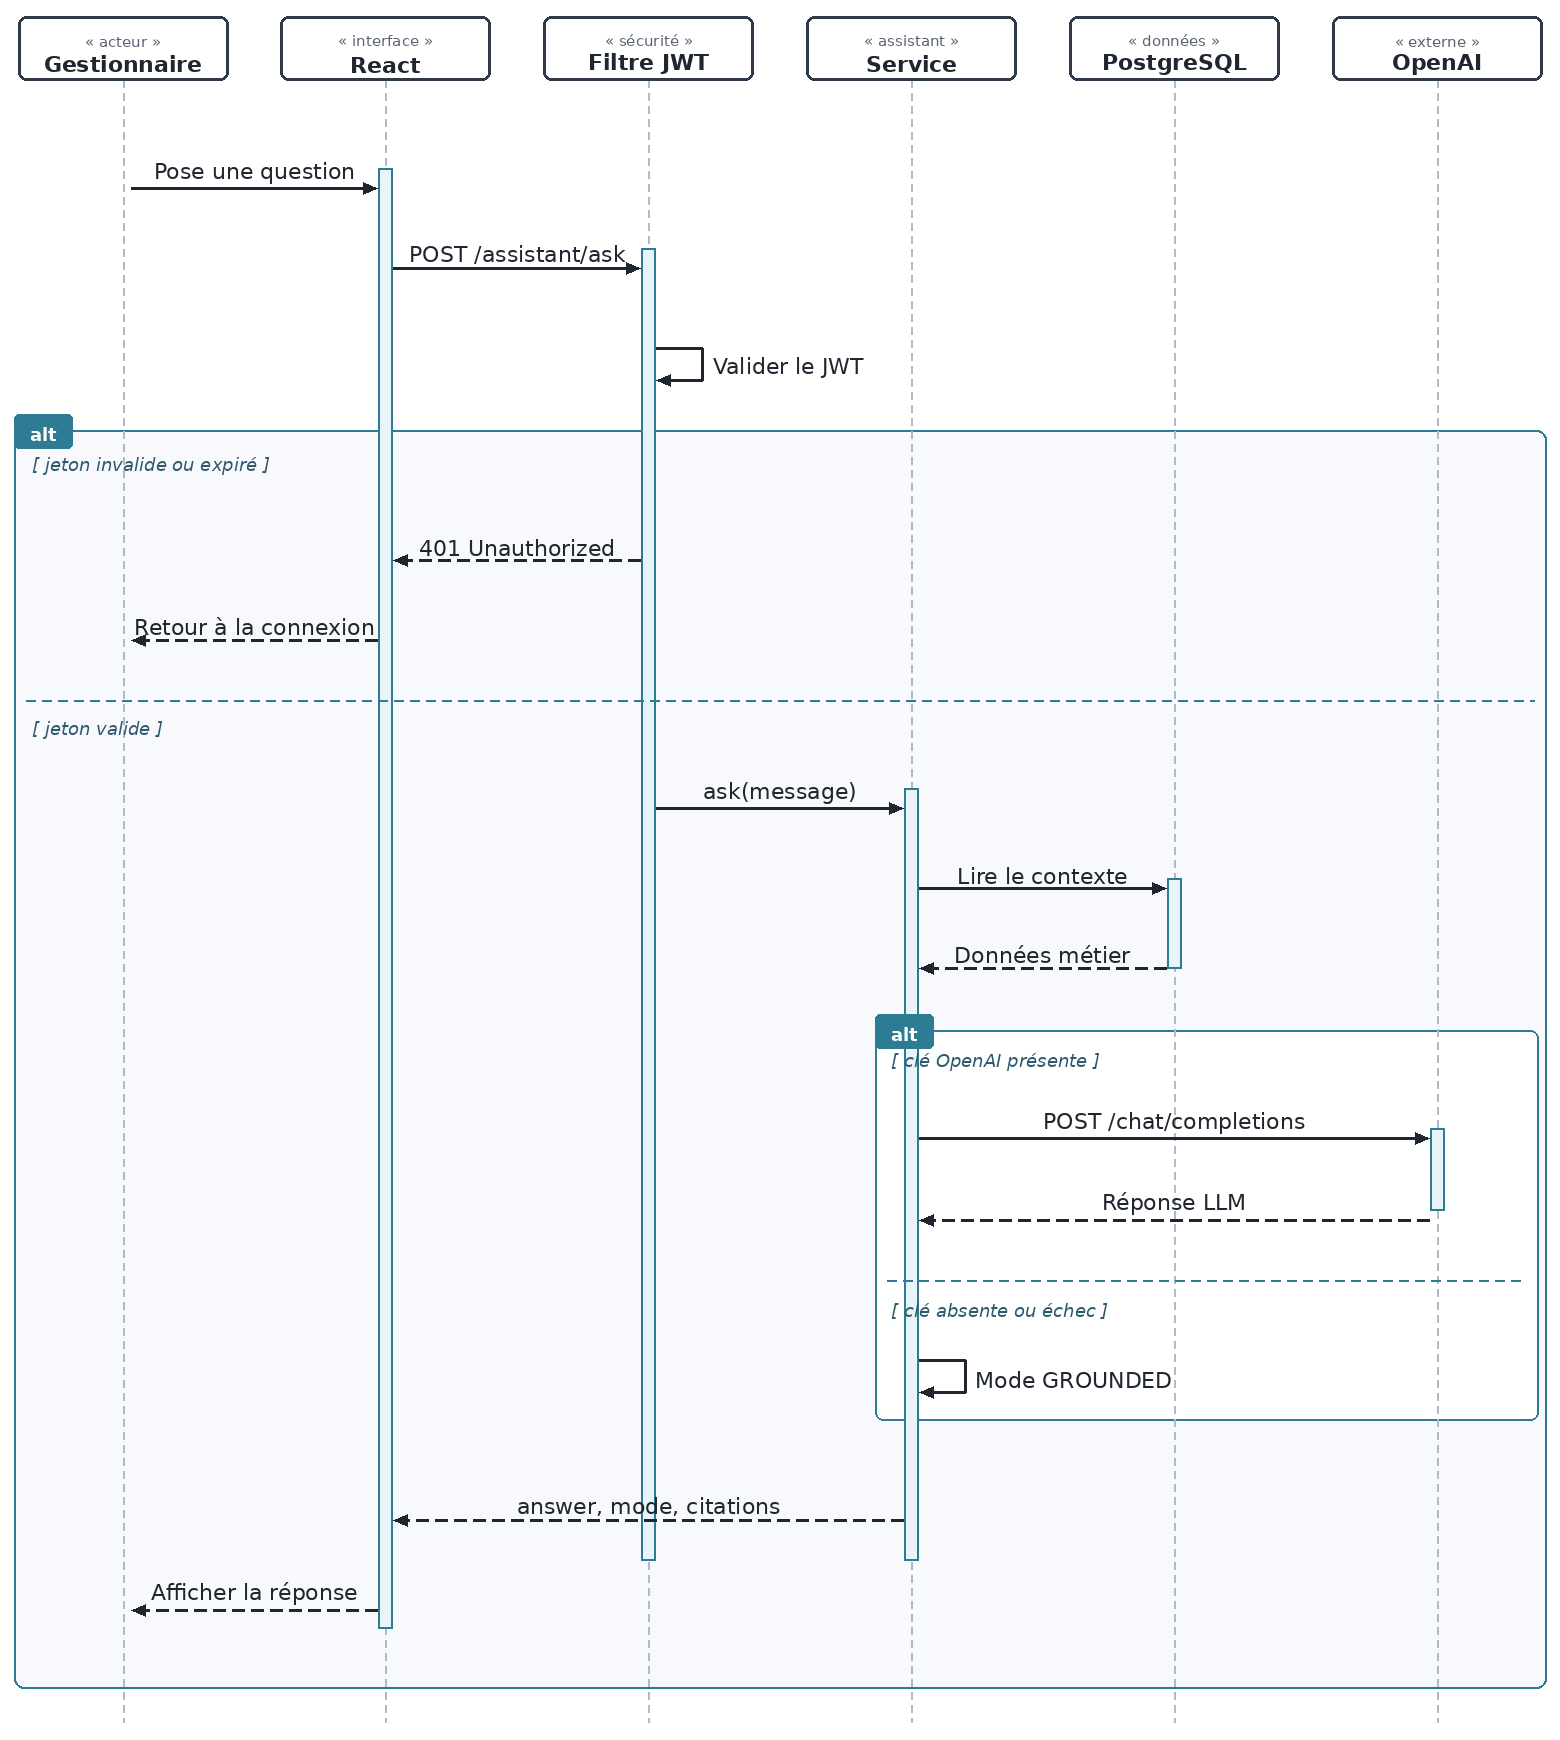
\includegraphics[width=\textwidth,keepaspectratio]{diagramme-sequence.png}%
}{%
  \FigPlaceholder{Générer \texttt{docs/soutenance/draw\_sequence\_assistant.py}\\vers \texttt{docs/rapport-stage/figures/diagramme-sequence.png}}%
}
\caption{Diagramme de séquence de la question à l'assistant IA}
\label{fig:seq-assistant}
\end{figure}

\clearpage
\section{Diagramme de classes}

\subsection{Entités du domaine}

\begin{figure}[htbp]
\centering
\IfFileExists{figures/diagramme-classes.png}{%
  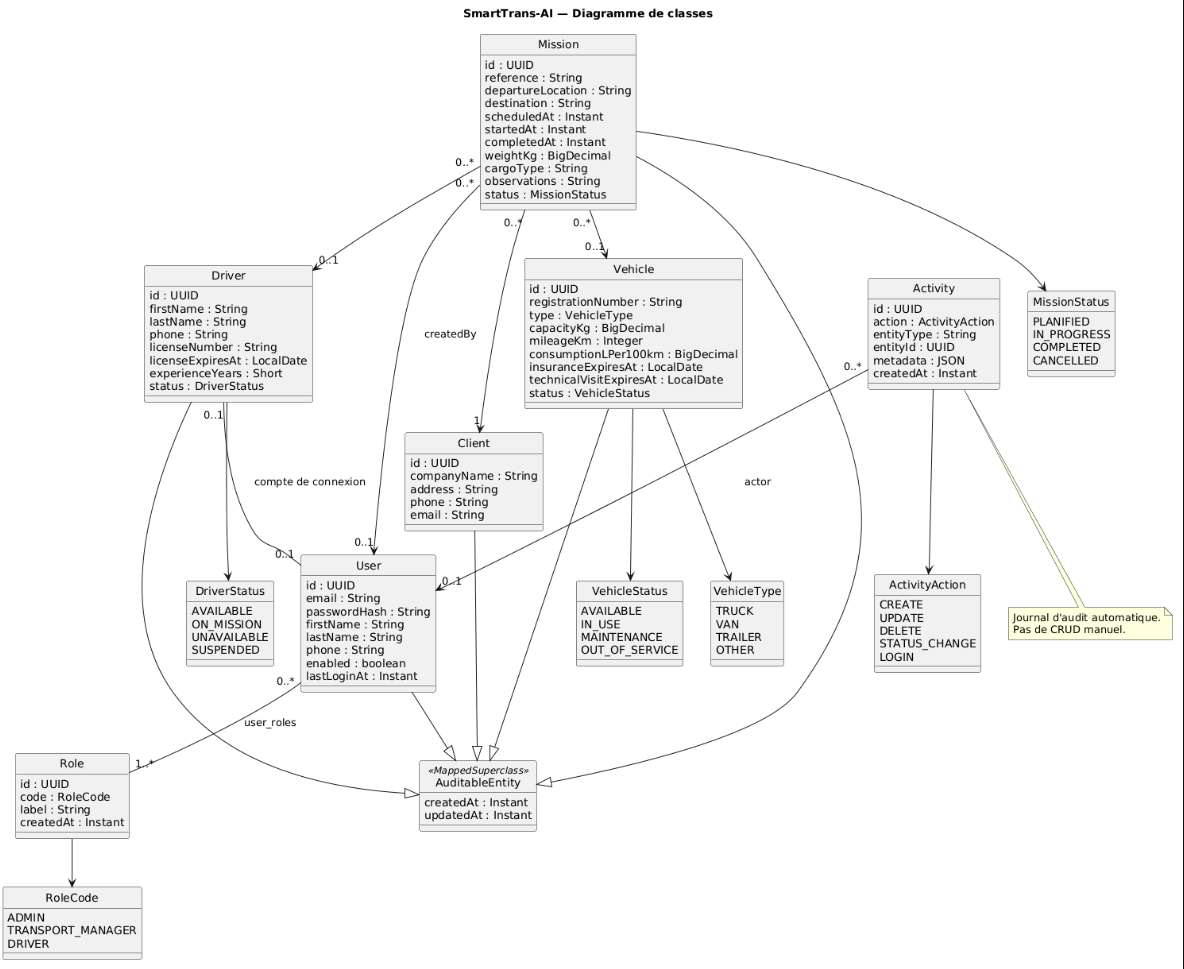
\includegraphics[width=0.92\textwidth]{diagramme-classes.png}%
}{%
  \FigPlaceholder{Exporter \texttt{docs/rapport/diagramme-classes.puml} en PNG\\vers \texttt{docs/rapport-stage/figures/diagramme-classes.png}}%
}
\caption{Diagramme de classes du domaine SmartTrans-AI}
\label{fig:classes}
\end{figure}

Le diagramme de la figure~\ref{fig:classes} représente le domaine persisté de SmartTrans-AI. Au centre, la classe \texttt{Mission} matérialise une course : référence, trajet, dates, tonnage et statut. Elle dépend d'un \texttt{Client} obligatoire et, le cas échéant, d'un \texttt{Driver} et d'un \texttt{Vehicle} ; l'association \texttt{createdBy} mémorise l'utilisateur qui a planifié la course. \texttt{User} et \texttt{Role} sont reliés par une association plusieurs-à-plusieurs (\texttt{user\_roles}), ce qui permet d'attribuer un ou plusieurs profils (administrateur, responsable transport, chauffeur). Un \texttt{Driver} peut être lié à au plus un compte \texttt{User}, afin que le chauffeur se connecte et suive uniquement ses missions. \texttt{Activity} constitue le journal d'audit : chaque action (création, mise à jour, suppression, changement de statut, connexion) pointe vers l'acteur. Les classes métier héritent de \texttt{AuditableEntity} (\texttt{createdAt}, \texttt{updatedAt}). Les énumérations \texttt{RoleCode}, \texttt{DriverStatus}, \texttt{VehicleStatus}, \texttt{VehicleType}, \texttt{MissionStatus} et \texttt{ActivityAction} limitent les valeurs autorisées. Les modules Document et Notification, hors périmètre livré, n'apparaissent pas sur ce diagramme.

\section{Modèle de données}

Les tables PostgreSQL correspondent aux classes : \texttt{users}, \texttt{roles}, \texttt{user\_roles}, \texttt{clients}, \texttt{drivers}, \texttt{vehicles}, \texttt{missions}, \texttt{activities}. Les identifiants sont des UUID. Le schéma est versionné par Flyway (validation au démarrage hors profil de test). Le tableau~\ref{tab:tables} synthétise les relations.

\begin{table}[htbp]
\centering
\caption{Principales relations du schéma}
\label{tab:tables}
\begin{tabular}{|p{0.28\textwidth}|p{0.28\textwidth}|p{0.34\textwidth}|}
\hline
\TableHead
\tht{Table} & \tht{Lien} & \tht{Cardinalité} \\
\hline
\texttt{user\_roles} & users -- roles & $n$--$n$ \\
\hline
\texttt{drivers.user\_id} & drivers -- users & $0..1$--$0..1$ \\
\hline
\texttt{missions.client\_id} & missions -- clients & $n$--$1$ \\
\hline
\texttt{missions.driver\_id} & missions -- drivers & $n$--$0..1$ \\
\hline
\texttt{missions.vehicle\_id} & missions -- vehicles & $n$--$0..1$ \\
\hline
\texttt{activities.actor\_user\_id} & activities -- users & $n$--$0..1$ \\
\hline
\end{tabular}
\end{table}

\section{Architecture logicielle}

L'interface React s'exécute dans le navigateur. En développement, le serveur Vite (port 5173) transmet les appels \texttt{/api} vers Spring Boot (port 8080). En production conteneurisée, un serveur HTTP (Nginx) sert les fichiers statiques et reverse-proxifie l'API. PostgreSQL stocke le métier. Le schéma~\ref{sch:arch} résume les flux.

\begin{schema}[htbp]
\centering
\fbox{%
\begin{minipage}{0.94\textwidth}
\centering\vspace{0.85cm}
\begin{tabular}{c@{\hspace{0.18cm}}c@{\hspace{0.18cm}}c@{\hspace{0.12cm}}c@{\hspace{0.12cm}}c@{\hspace{0.18cm}}c@{\hspace{0.18cm}}c@{\hspace{0.18cm}}c@{\hspace{0.18cm}}c}

\includegraphics[height=1.05cm]{logos/chrome.png} &
{\Large$\rightarrow$} &

\includegraphics[height=1.05cm]{logos/react.png} &
{\large/} &

\includegraphics[height=0.70cm]{logos/nginx.png} &
{\Large$\rightarrow$} &

\includegraphics[height=1.05cm]{logos/spring.png} &
{\Large$\rightarrow$} &

\includegraphics[height=1.05cm]{logos/postgresql.png} \\[0.28cm]
\small Navigateur && \small React && \small Nginx && \small Spring Boot && \small PostgreSQL
\end{tabular}
\vspace{0.85cm}
\end{minipage}%
}
\caption{Architecture logique de SmartTrans-AI}
\label{sch:arch}
\end{schema}

\section{Conclusion}

L'analyse produit un système à trois acteurs, un domaine centré sur la mission, et une architecture présentation / API / données. Le chapitre suivant décrit la traduction de cette conception en logiciel.

\chapter{Réalisation}

\section{Introduction}

Ce chapitre présente la mise en œuvre : sécurité, modules métier, interface selon le rôle, assistant et journal d'activités.

\section{Authentification et sécurité}

L'utilisateur s'identifie par courriel et mot de passe. Le serveur vérifie le mot de passe haché, génère un JWT et le client le transmet dans l'en-tête \texttt{Authorization}. Les routes \texttt{/api/v1/auth/} restent accessibles sans jeton. Le jeton suit le standard JWT \cite{jwt}. La configuration CORS autorise les origines locales (\texttt{localhost} et \texttt{127.0.0.1}) afin que le front de développement puisse appeler l'API. Les contrôleurs restreignent les opérations selon les autorités Spring Security correspondant aux rôles.

\section{Gestion des utilisateurs et des rôles}

L'administrateur crée et met à jour les comptes, active ou désactive un utilisateur, et assigne un ou plusieurs rôles. Cette fonction n'est pas exposée au responsable transport ni au chauffeur, afin de limiter la surface d'administration.

\section{Clients, chauffeurs et véhicules}

\subsection{Clients}

Un client est identifié par le nom de l'entreprise, une adresse, un téléphone et un courriel optionnel. Il est obligatoire sur chaque mission.

\subsection{Chauffeurs}

Le chauffeur porte un numéro de permis, une date d'expiration, une ancienneté et un statut (disponible, en mission, indisponible, suspendu). Le lien optionnel avec un \texttt{User} permet la connexion à l'espace chauffeur.

\subsection{Véhicules}

Le véhicule est caractérisé par l'immatriculation, le type, la capacité, le kilométrage, des dates d'assurance et de visite technique, et un statut d'exploitation. Ces dates alimentent les rappels du tableau de bord.

\section{Missions}

La mission possède une référence unique, un trajet (départ, destination), une date planifiée, un tonnage et un type de marchandise optionnels. Le responsable et l'administrateur créent et modifient les champs. Le changement de statut du chauffeur passe par une ressource dédiée : il peut passer une mission qui lui est affectée de planifiée à en cours, puis à terminée. L'annulation reste du ressort de l'exploitation.

\section{Tableau de bord, alertes et journal}

Le tableau de bord affiche des indicateurs, des graphiques (activité de la semaine, répartition des statuts), les prochaines missions et les rappels (permis, assurance, contrôle technique). Le journal d'activités liste les événements avec un libellé d'objet lisible (référence de mission, nom, immatriculation, entreprise, courriel) plutôt qu'un identifiant technique seul.

\section{Assistant IA}

L'assistant est réservé à l'administrateur et au responsable transport. Il s'appuie sur un extrait des missions, chauffeurs, véhicules et clients. Lorsqu'une clé de modèle de langage est configurée, les réponses sont générées à partir de ce contexte ; sinon, des règles déterministes couvrent les questions fréquentes (effectifs, suggestions). L'objectif pédagogique et opérationnel est d'«~ancrer~» l'IA sur le SI, afin de limiter les hallucinations. Les échanges correspondants sont ceux de la figure~\ref{fig:seq-assistant}.

\section{Organisation du code et API}

Le backend est structuré par packages métier (\texttt{auth}, \texttt{user}, \texttt{role}, \texttt{client}, \texttt{driver}, \texttt{vehicle}, \texttt{mission}, \texttt{activity}, assistant). Chaque module typique expose un contrôleur REST, un service et un dépôt JPA. Le préfixe public est \texttt{/api/v1}. Le tableau~\ref{tab:api} donne un extrait des ressources.

\begin{table}[htbp]
\centering
\caption{Extrait des ressources REST}
\label{tab:api}
\begin{tabular}{|p{0.40\textwidth}|p{0.18\textwidth}|p{0.32\textwidth}|}
\hline
\TableHead
\tht{Ressource} & \tht{Méthode} & \tht{Usage} \\
\hline
\texttt{/auth/login} & POST & Authentification, JWT \\
\hline
\texttt{/users} & GET, POST, PATCH & Comptes (admin) \\
\hline
\texttt{/clients}, \texttt{/drivers}, \texttt{/vehicles} & CRUD & Référentiels \\
\hline
\texttt{/missions} & CRUD & Planification \\
\hline
\texttt{/missions/\{id\}/status} & PATCH & Statut (dont chauffeur) \\
\hline
\texttt{/activities} & GET & Journal lecture seule \\
\hline
\texttt{/assistant} & POST & Question / suggestions \\
\hline
\end{tabular}
\end{table}

Les écrans React (listes, formulaires, tableau de bord, assistant) consomment ces ressources via un client HTTP unique, qui attache le jeton sauf sur le login.

\section{Interface utilisateur}

L'interface distingue la navigation : le chauffeur accède au tableau de bord, à ses missions et à son profil ; les autres rôles voient en plus les menus d'exploitation, le journal et l'assistant. Les formulaires de saisie et les listes correspondent aux ressources de l'API. Les messages d'erreur HTTP (par exemple un refus d'authentification) sont traduits pour l'utilisateur.

\section{Conclusion}

La réalisation couvre la chaîne authentification--métier--pilotage--assistant, avec une séparation claire des droits. Le chapitre suivant évalue la qualité logicielle et le déploiement.

\chapter{Tests, déploiement et discussion}

\section{Introduction}

Ce chapitre présente la stratégie de tests, les modalités de déploiement, les difficultés rencontrées et les limites du livrable.

\section{Stratégie de tests}

Le backend dispose de tests Maven. Le profil de test utilise H2 pour une partie des cas ; des tests d'intégration s'appuient sur PostgreSQL embarqué afin de valider Flyway et JPA. Des scénarios HTTP couvrent l'authentification JWT et des exemples de CRUD (utilisateurs). Cette base ne remplace pas une recette métier complète mais sécurise les régressions sur la sécurité et la persistance.

\subsection{Scénarios de recette}

Le tableau~\ref{tab:recette} propose une grille de recette manuelle, utilisable lors d'une démonstration à S. WATRANS.

\begin{table}[htbp]
\centering
\caption{Grille de recette fonctionnelle (extrait)}
\label{tab:recette}
\begin{tabular}{|p{0.08\textwidth}|p{0.42\textwidth}|p{0.40\textwidth}|}
\hline
\TableHead
\tht{Id} & \tht{Scénario} & \tht{Résultat attendu} \\
\hline
R1 & Login admin valide & Accès dashboard et menus d'admin \\
\hline
R2 & Login chauffeur & Menus limités (missions, profil) \\
\hline
R3 & Création mission + client & Mission planifiée, trace d'audit \\
\hline
R4 & Chauffeur démarre puis termine & Statuts et dates mis à jour \\
\hline
R5 & Chauffeur tente une annulation & Refus (droit insuffisant) \\
\hline
R6 & Permis ou assurance proche & Alerte sur le tableau de bord \\
\hline
R7 & Question « combien de missions » & Réponse courte, cohérente avec la base \\
\hline
R8 & Login erroné & Message clair, pas d'accès \\
\hline
\end{tabular}
\end{table}

\section{Déploiement}

En développement, PostgreSQL peut être lancé via Docker Compose, l'API par Maven, l'interface par \texttt{npm run dev}. Une stack de production assemble base, API et Nginx (port d'écoute distinct, par exemple 8088). Les secrets (mot de passe de base, secret JWT, clé d'API éventuelle) doivent être fournis par variables d'environnement et non versionnés. Un compte administrateur peut être créé au premier démarrage si la base est vide (\textit{bootstrap}), ce qui facilite une démonstration.

\section{Difficultés et solutions}

Plusieurs points ont demandé un diagnostic : autorisation CORS entre \texttt{localhost} et \texttt{127.0.0.1}, envoi d'un jeton Bearer sur la route de login, messages d'erreur 403 peu lisibles, alimentation du tableau de bord par des données de démonstration. Chaque correctif a visé un comportement prévisible pour l'utilisateur final (connexion depuis le front de développement, listes et graphiques non vides).

\section{Limites et perspectives}

Le livrable n'inclut pas de bus d'événements (Kafka), ni de notifications temps réel, ni de module documentaire. L'assistant dépend de la qualité du contexte injecté et, le cas échéant, d'un prestataire de modèle de langage. Un durcissement (HTTPS, secrets, politique de mots de passe, journalisation centralisée) reste souhaitable avant un usage en production réelle. Ces pistes peuvent faire l'objet d'un travail ultérieur.

\section{Conclusion}

Les tests automatisés et le déploiement local ou conteneurisé rendent le projet démontrable. Les limites rappellent qu'il s'agit d'un produit de stage, extensible. Le chapitre suivant revient sur le planning, les risques et les livrables.

\chapter{Conduite de projet}

\section{Introduction}

La réalisation de SmartTrans-AI s'est inscrite dans une démarche itérative, compatible avec un stage en entreprise : lots fonctionnels successifs, recette interne, puis rédaction du rapport. Ce chapitre présente le découpage, les risques et les livrables.

\section{Méthode de travail}

Le travail a suivi un cycle proche de l'agilité légère : expression du besoin avec l'encadrante entreprise, maquettes et API, développement par module (authentification, référentiels, missions, tableau de bord, journal, assistant), puis ajustements (droits chauffeur, CORS, messages d'erreur). Les diagrammes UML ont servi de contrat entre l'analyse et le code. Les tests automatisés du backend ont été exécutés à chaque palier critique (sécurité, persistance).

\section{Planning prévisionnel}

Le tableau~\ref{tab:planning} présente le découpage du projet sur un mois de stage (quatre semaines). L'ordre des lots correspond à la dépendance technique (on n'expose pas les missions sans authentification).

\begin{table}[htbp]
\centering
\caption{Découpage du projet en lots}
\label{tab:planning}
\begin{tabular}{|p{0.14\textwidth}|p{0.38\textwidth}|p{0.38\textwidth}|}
\hline
\TableHead
\tht{Période} & \tht{Lot} & \tht{Résultat attendu} \\
\hline
Semaine 1 & Cadre, besoin, rôles, modèle de données, sécurité JWT & Cahier des charges interne, schéma Flyway, login \\
\hline
Semaine 2 & Utilisateurs, clients, chauffeurs, véhicules, missions & CRUD protégés, cycle de vie des courses \\
\hline
Semaine 3 & Tableau de bord, alertes, journal & Pilotage et traçabilité \\
\hline
Semaine 4 & Assistant, droits chauffeur, recette, Docker, rapport ENSIASD & Espace chauffeur, démo et mémoire \\
\hline
\end{tabular}
\end{table}

\Needspace{11cm}
\section{Risques et parades}

Cinq risques ont été suivis pendant le stage. Le tableau~\ref{tab:risques} indique, pour chacun, l'impact redouté et la parade appliquée.

\begin{center}
\captionof{table}{Risques principaux et parades}
\label{tab:risques}
\begin{tabular}{|p{0.30\textwidth}|p{0.22\textwidth}|p{0.38\textwidth}|}
\hline
\TableHead
\tht{Risque} & \tht{Impact} & \tht{Parade} \\
\hline
Périmètre trop large (GED, Kafka, notifications) & Retard & Priorisation du noyau métier \\
\hline
Hallucinations de l'assistant & Perte de confiance & Contexte SQL, réponses courtes, mode sans clé \\
\hline
Blocage CORS / JWT en local & Impossibilité de se connecter & Origines multiples, exclusion des routes d'auth \\
\hline
Données de démo vides & Tableau de bord peu lisible & Jeux de missions et alertes de démonstration \\
\hline
Dépendance à un prestataire LLM & Coût, indisponibilité & Mode déterministe local \\
\hline
\end{tabular}
\end{center}

\section{Livrables}

Les livrables du stage comprennent : le code source (backend Spring Boot, frontend React), le schéma de base, la documentation OpenAPI, les diagrammes UML, le présent rapport, et une procédure de démarrage local. Le produit reste un prototype d'entreprise, destiné à être repris par le département informatique.

\section{Conclusion}

La conduite de projet a privilégié un noyau démontrable plutôt qu'une couverture exhaustive du marché TMS. Cette discipline a permis d'aboutir à une application cohérente, testable et documentée. Le chapitre suivant présente les interfaces réalisées, écran par écran.

\chapter{Présentation des interfaces}

\section{Introduction}

Ce chapitre illustre le livrable tel qu'il apparaît à l'utilisateur. Les captures ont été réalisées sur l'environnement local (\texttt{http://127.0.0.1:5173}), avec le compte administrateur. Elles correspondent aux écrans du menu principal : connexion, tableau de bord, référentiels, missions, assistant, journal d'activités et administration. L'espace «~Mon profil~» du chauffeur n'est pas reproduit ici : il n'est accessible qu'avec un compte \texttt{DRIVER}.

\section{Connexion}

La figure~\ref{fig:ui-login} montre l'écran public de connexion. L'utilisateur saisit son courriel et son mot de passe. Un bouton unique déclenche l'appel d'authentification. En cas de succès, un jeton JWT est stocké côté client et l'application redirige vers le tableau de bord.

\begin{figure}[htbp]
\centering
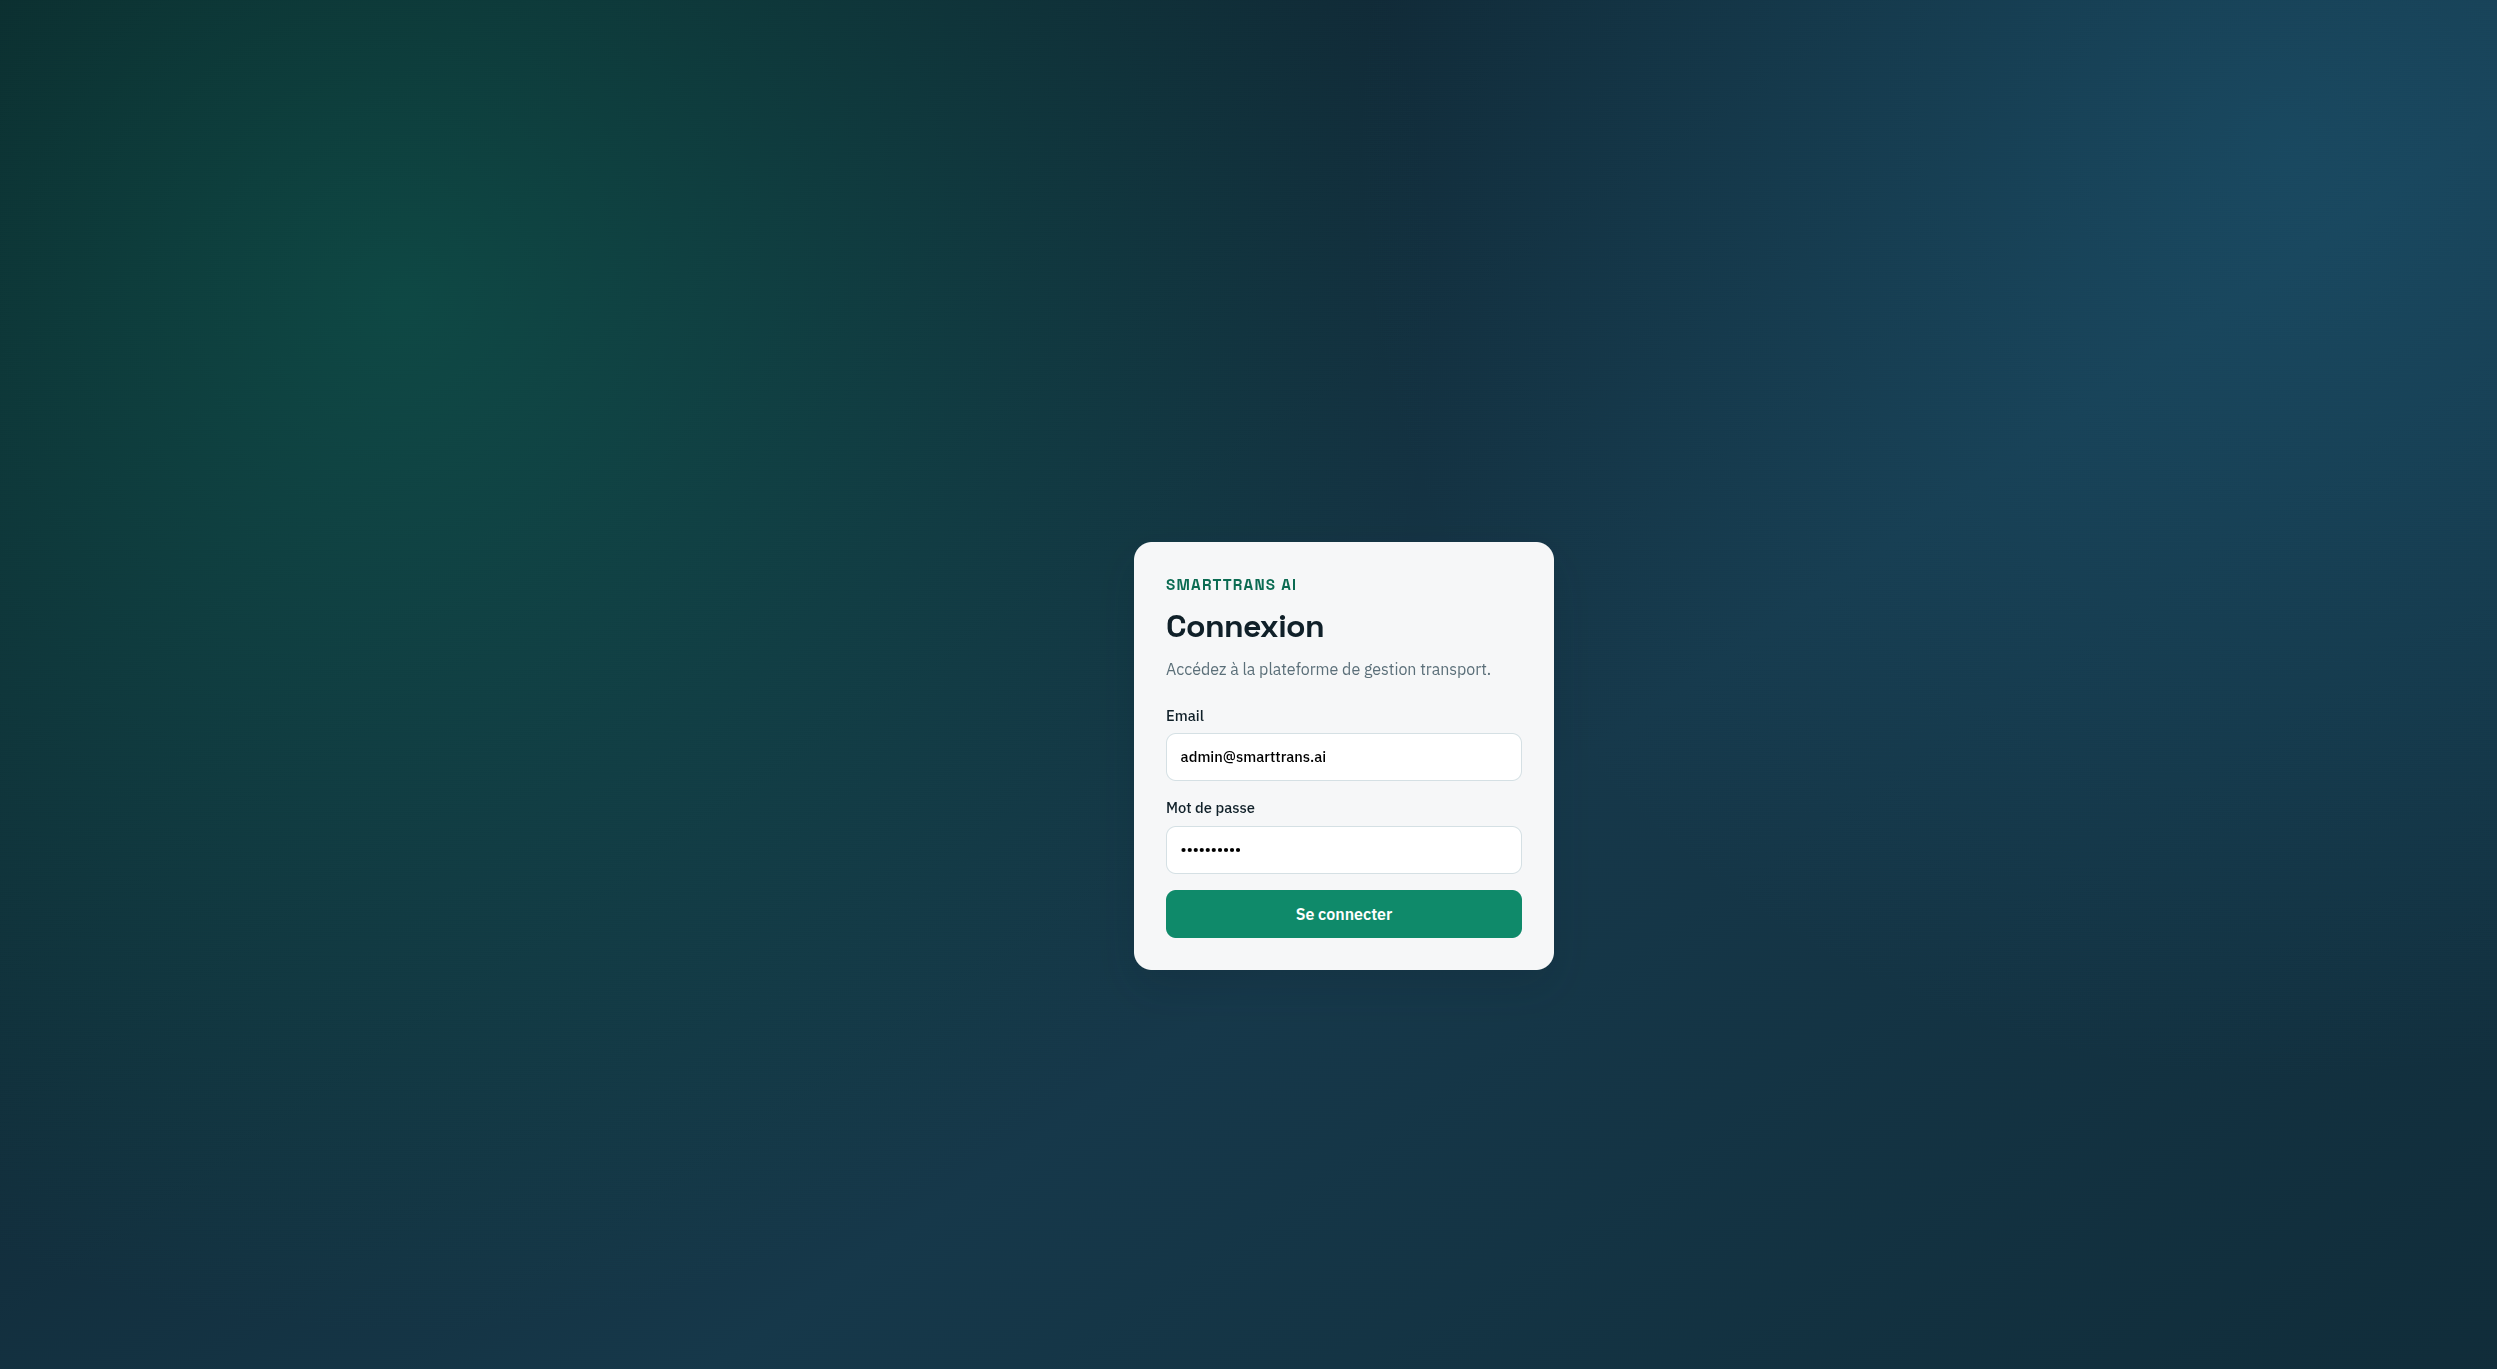
\includegraphics[width=0.82\textwidth,keepaspectratio]{ui-01-login.png}
\caption{Écran de connexion SmartTrans-AI}
\label{fig:ui-login}
\end{figure}

\section{Tableau de bord}

La figure~\ref{fig:ui-dash} présente la vue de pilotage. Les cartes du haut résument les volumes de missions, les ressources disponibles et les alertes (permis, assurance, visite technique). Les graphiques visualisent l'activité de la semaine et la répartition des statuts. Les listes du bas rappellent les prochaines courses, les chauffeurs en mission et les échéances.

\begin{figure}[htbp]
\centering
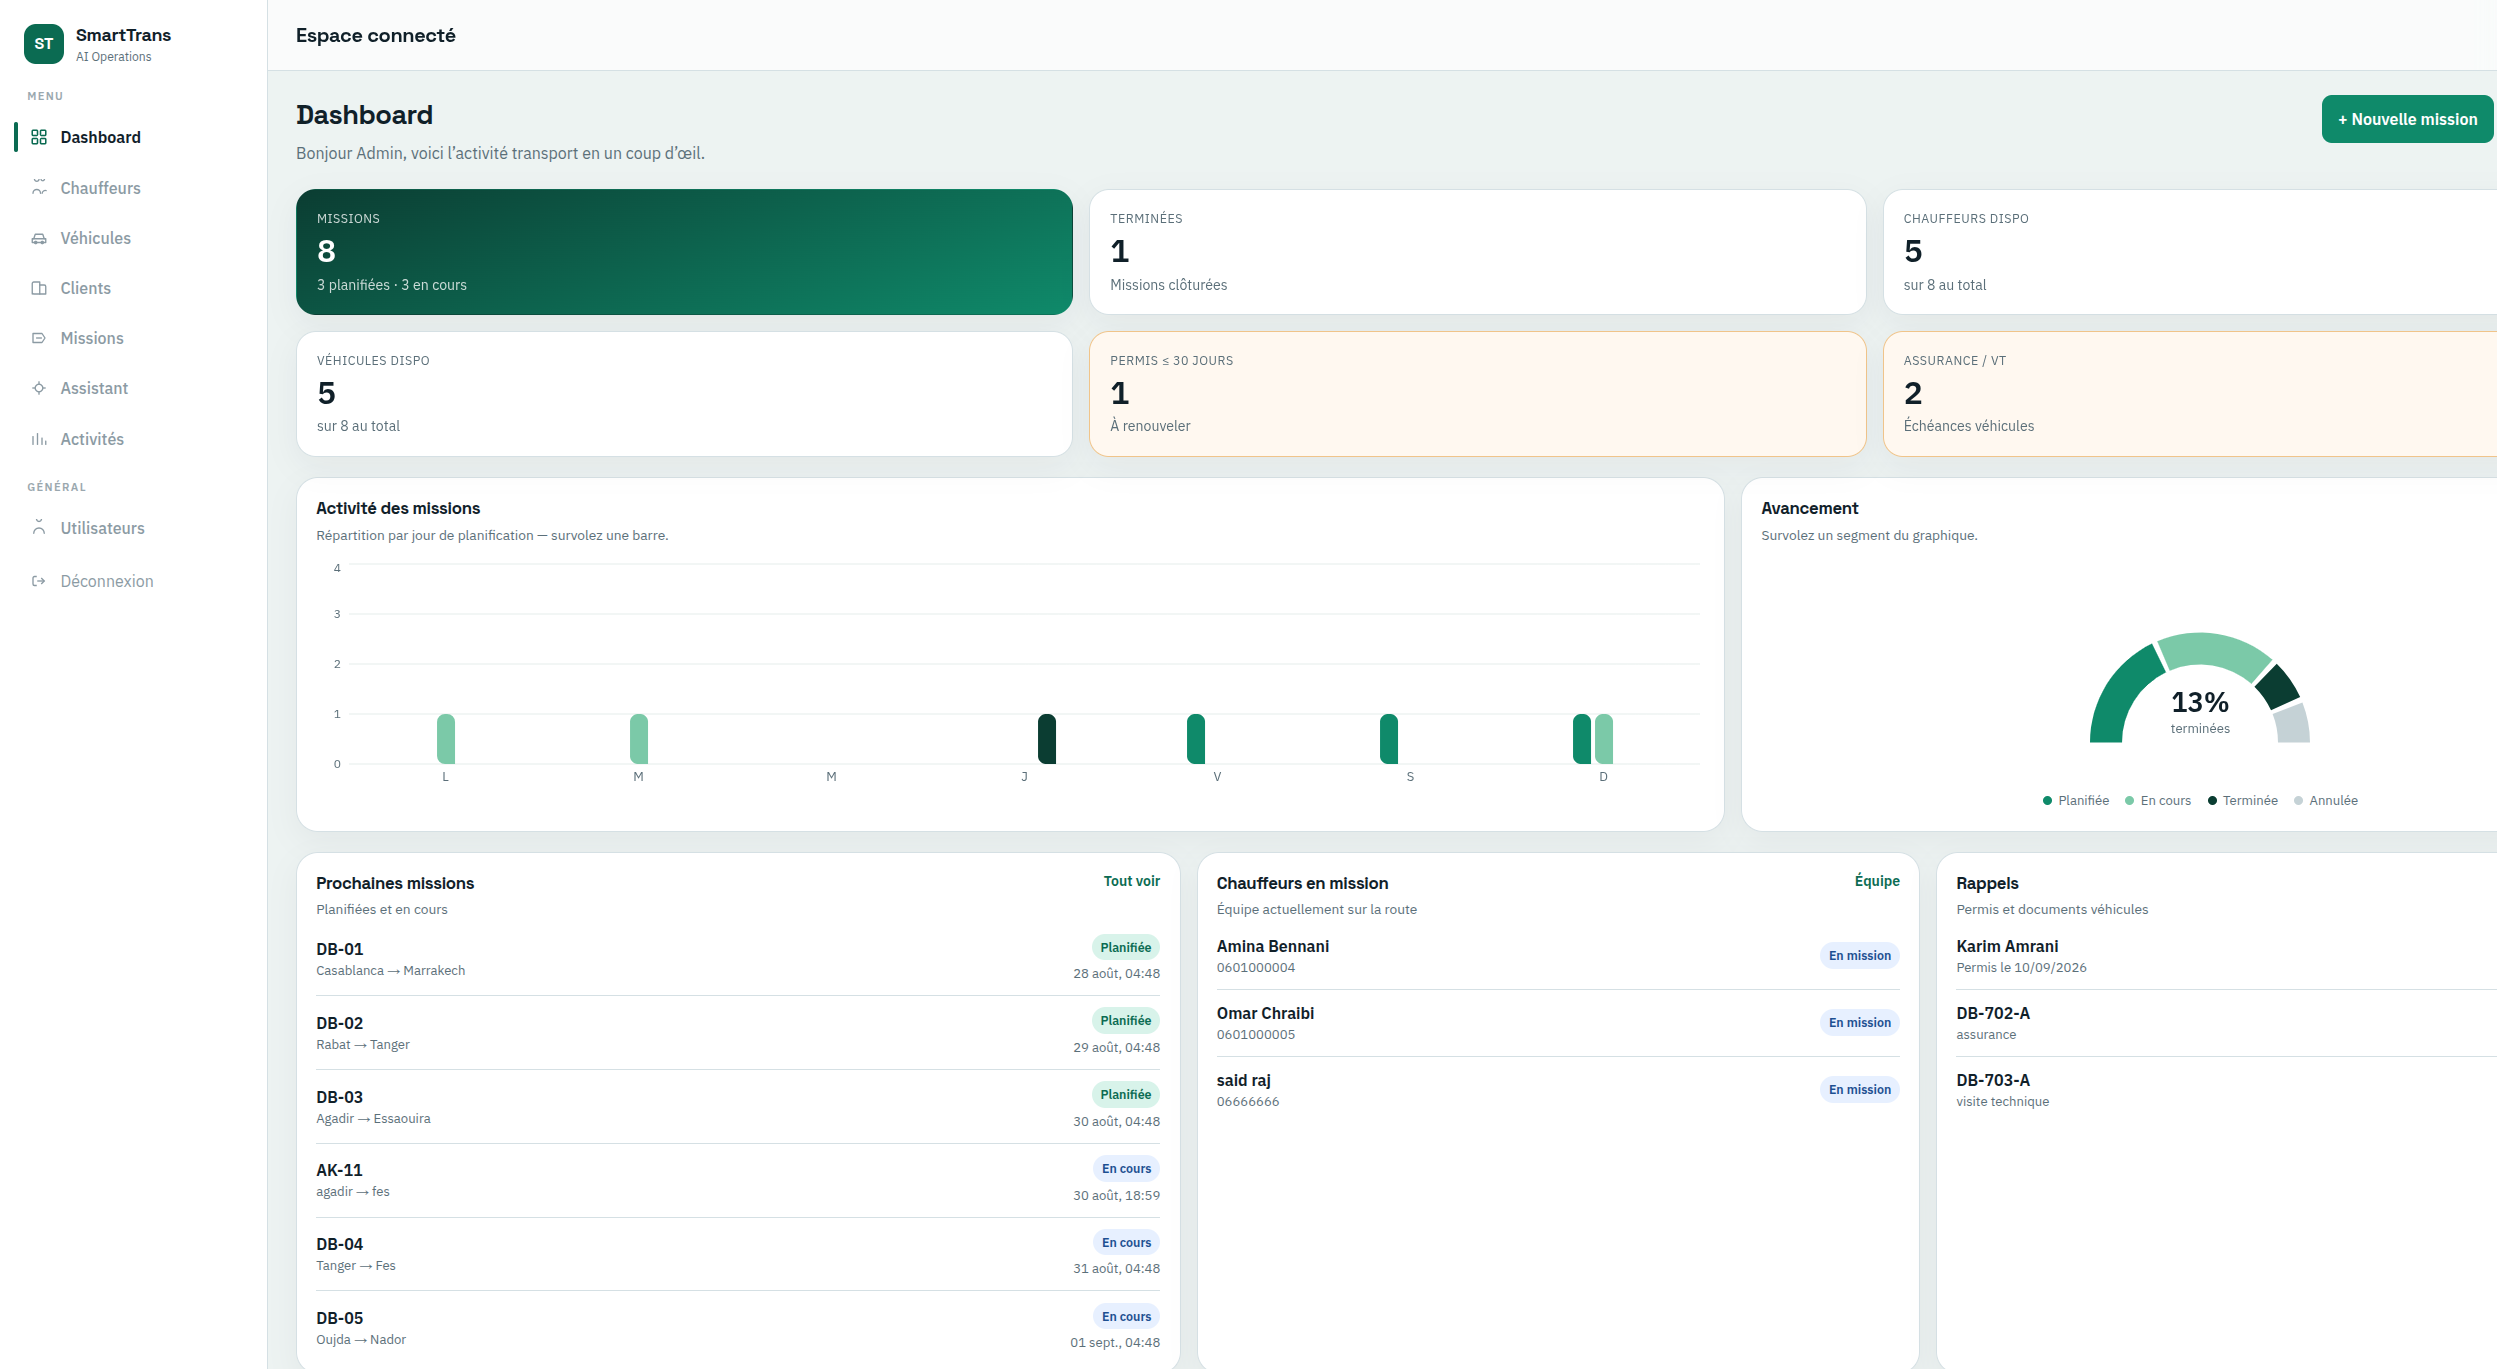
\includegraphics[width=0.95\textwidth,keepaspectratio]{ui-02-dashboard.png}
\caption{Tableau de bord (profil administrateur)}
\label{fig:ui-dash}
\end{figure}

\section{Gestion des chauffeurs}

La liste (figure~\ref{fig:ui-drv-list}) permet de rechercher un chauffeur, de filtrer par statut et par échéance de permis. La création (figure~\ref{fig:ui-drv-new}) saisit l'identité, le permis et le statut. Le détail (figure~\ref{fig:ui-drv-det}) affiche les rappels d'expiration. La modification (figure~\ref{fig:ui-drv-edit}) reprend le même formulaire prérempli.

\begin{figure}[htbp]
\centering
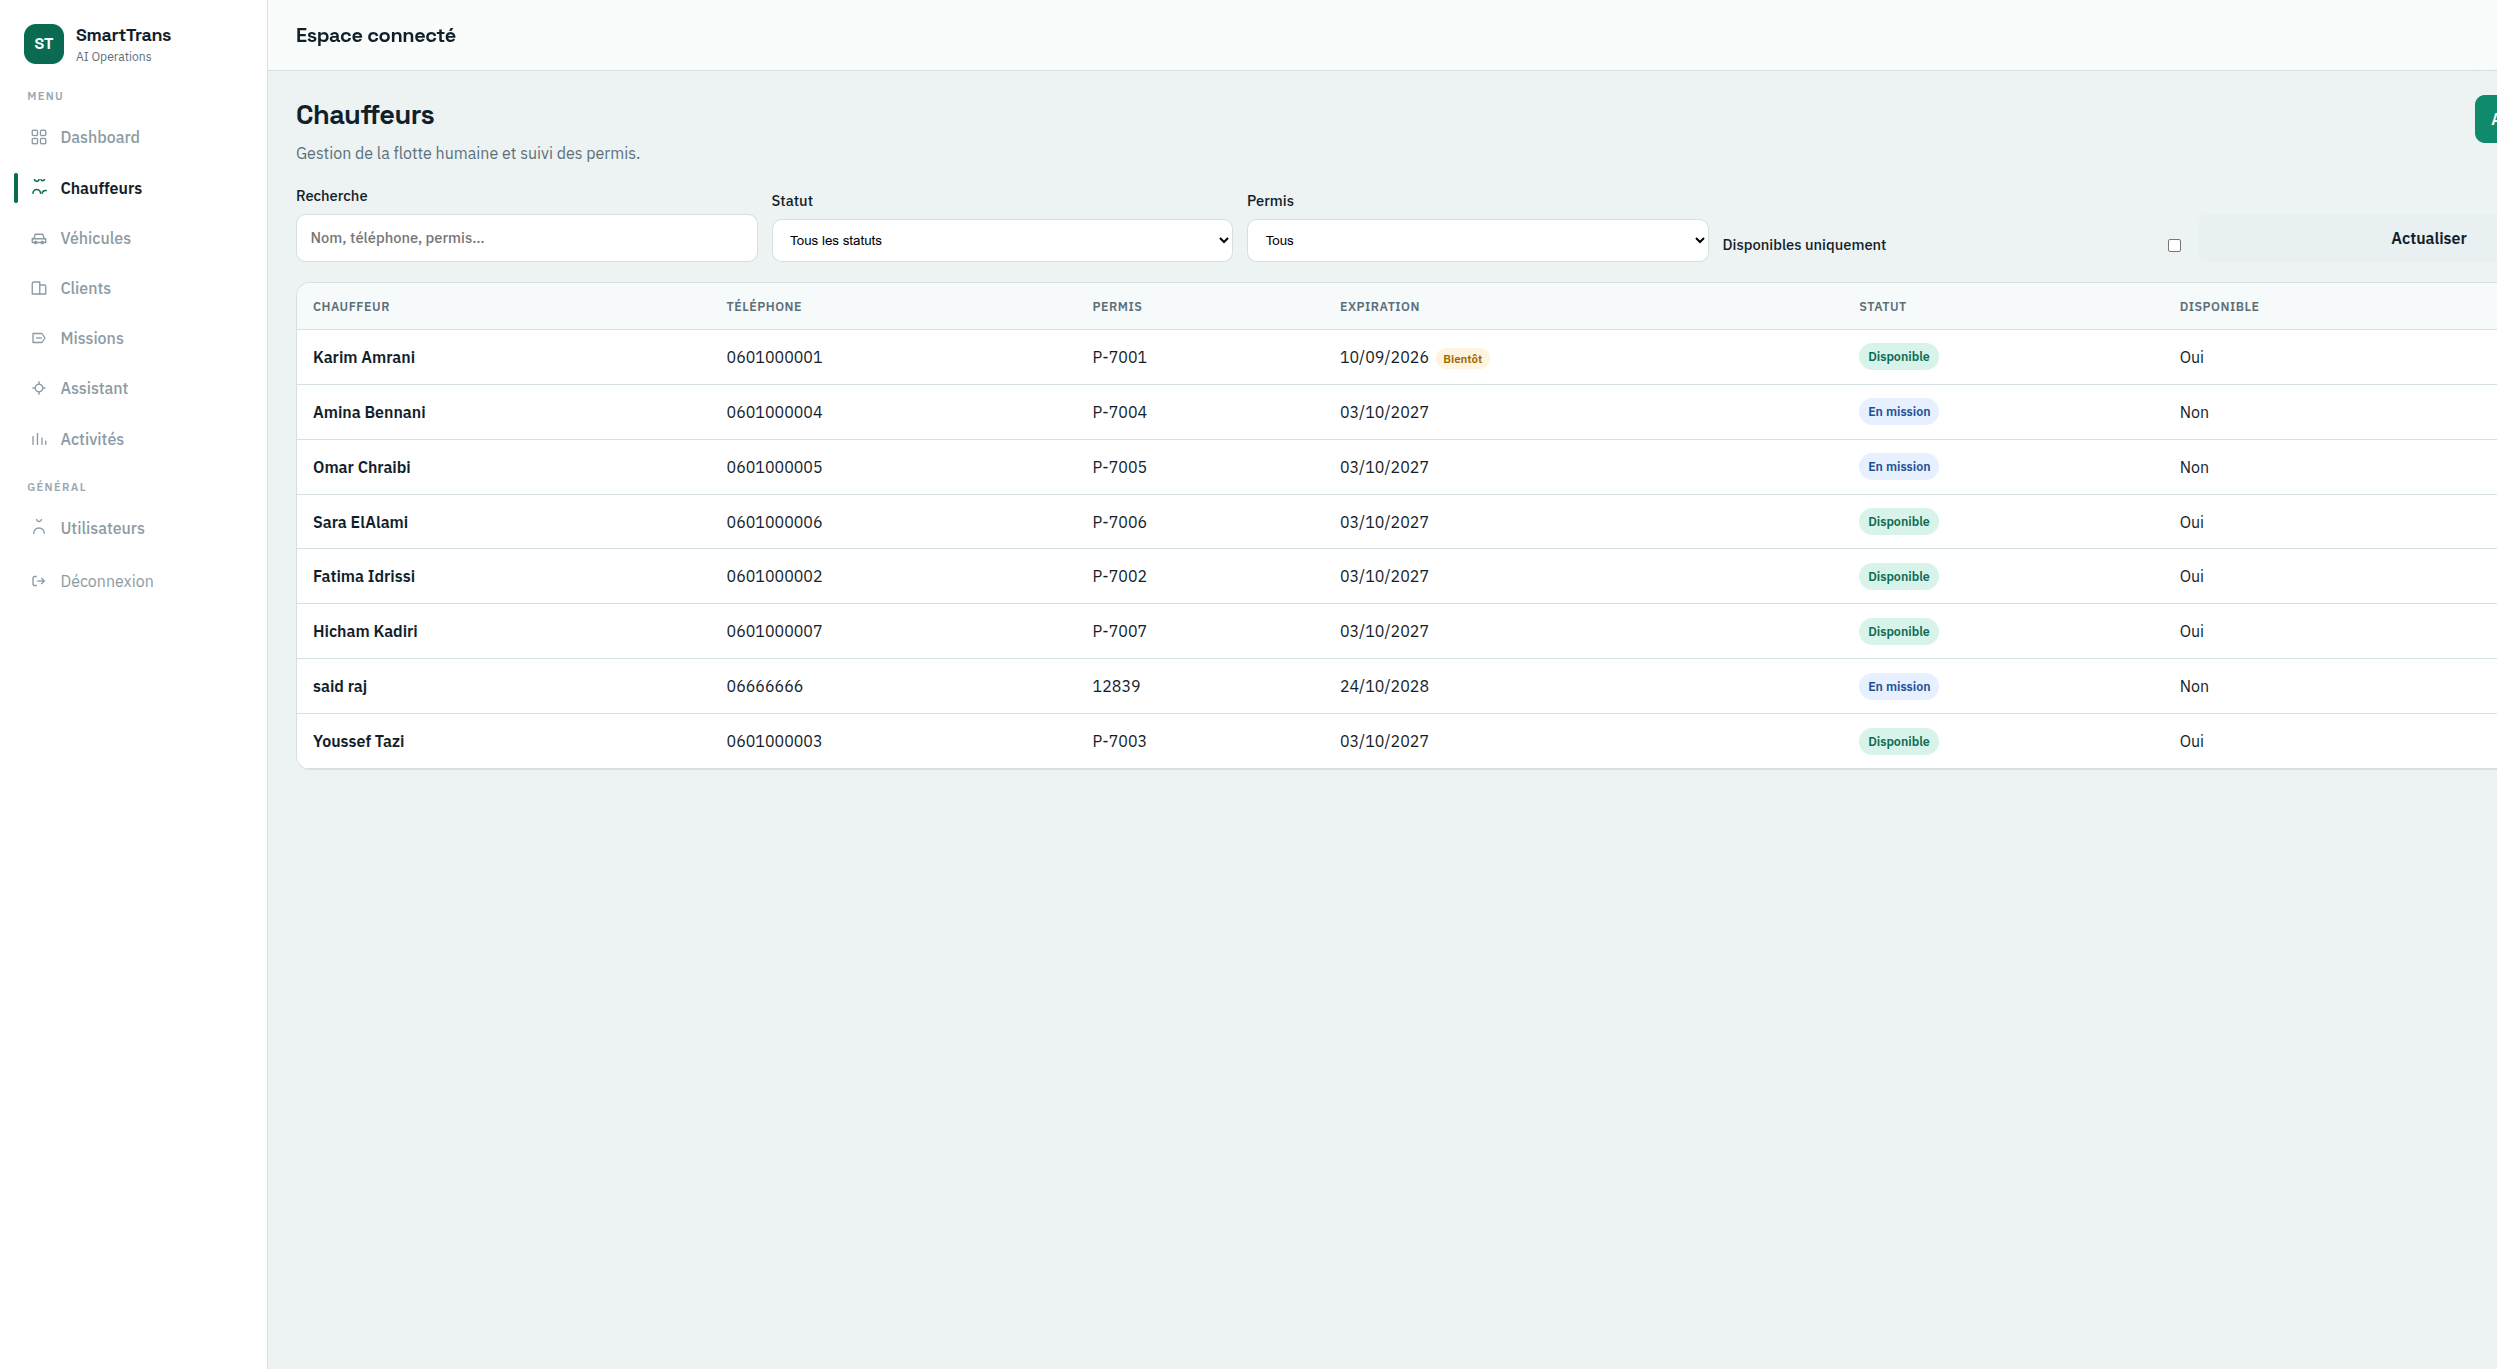
\includegraphics[width=0.95\textwidth,keepaspectratio]{ui-03-chauffeurs.png}
\caption{Liste des chauffeurs}
\label{fig:ui-drv-list}
\end{figure}

\begin{figure}[htbp]
\centering
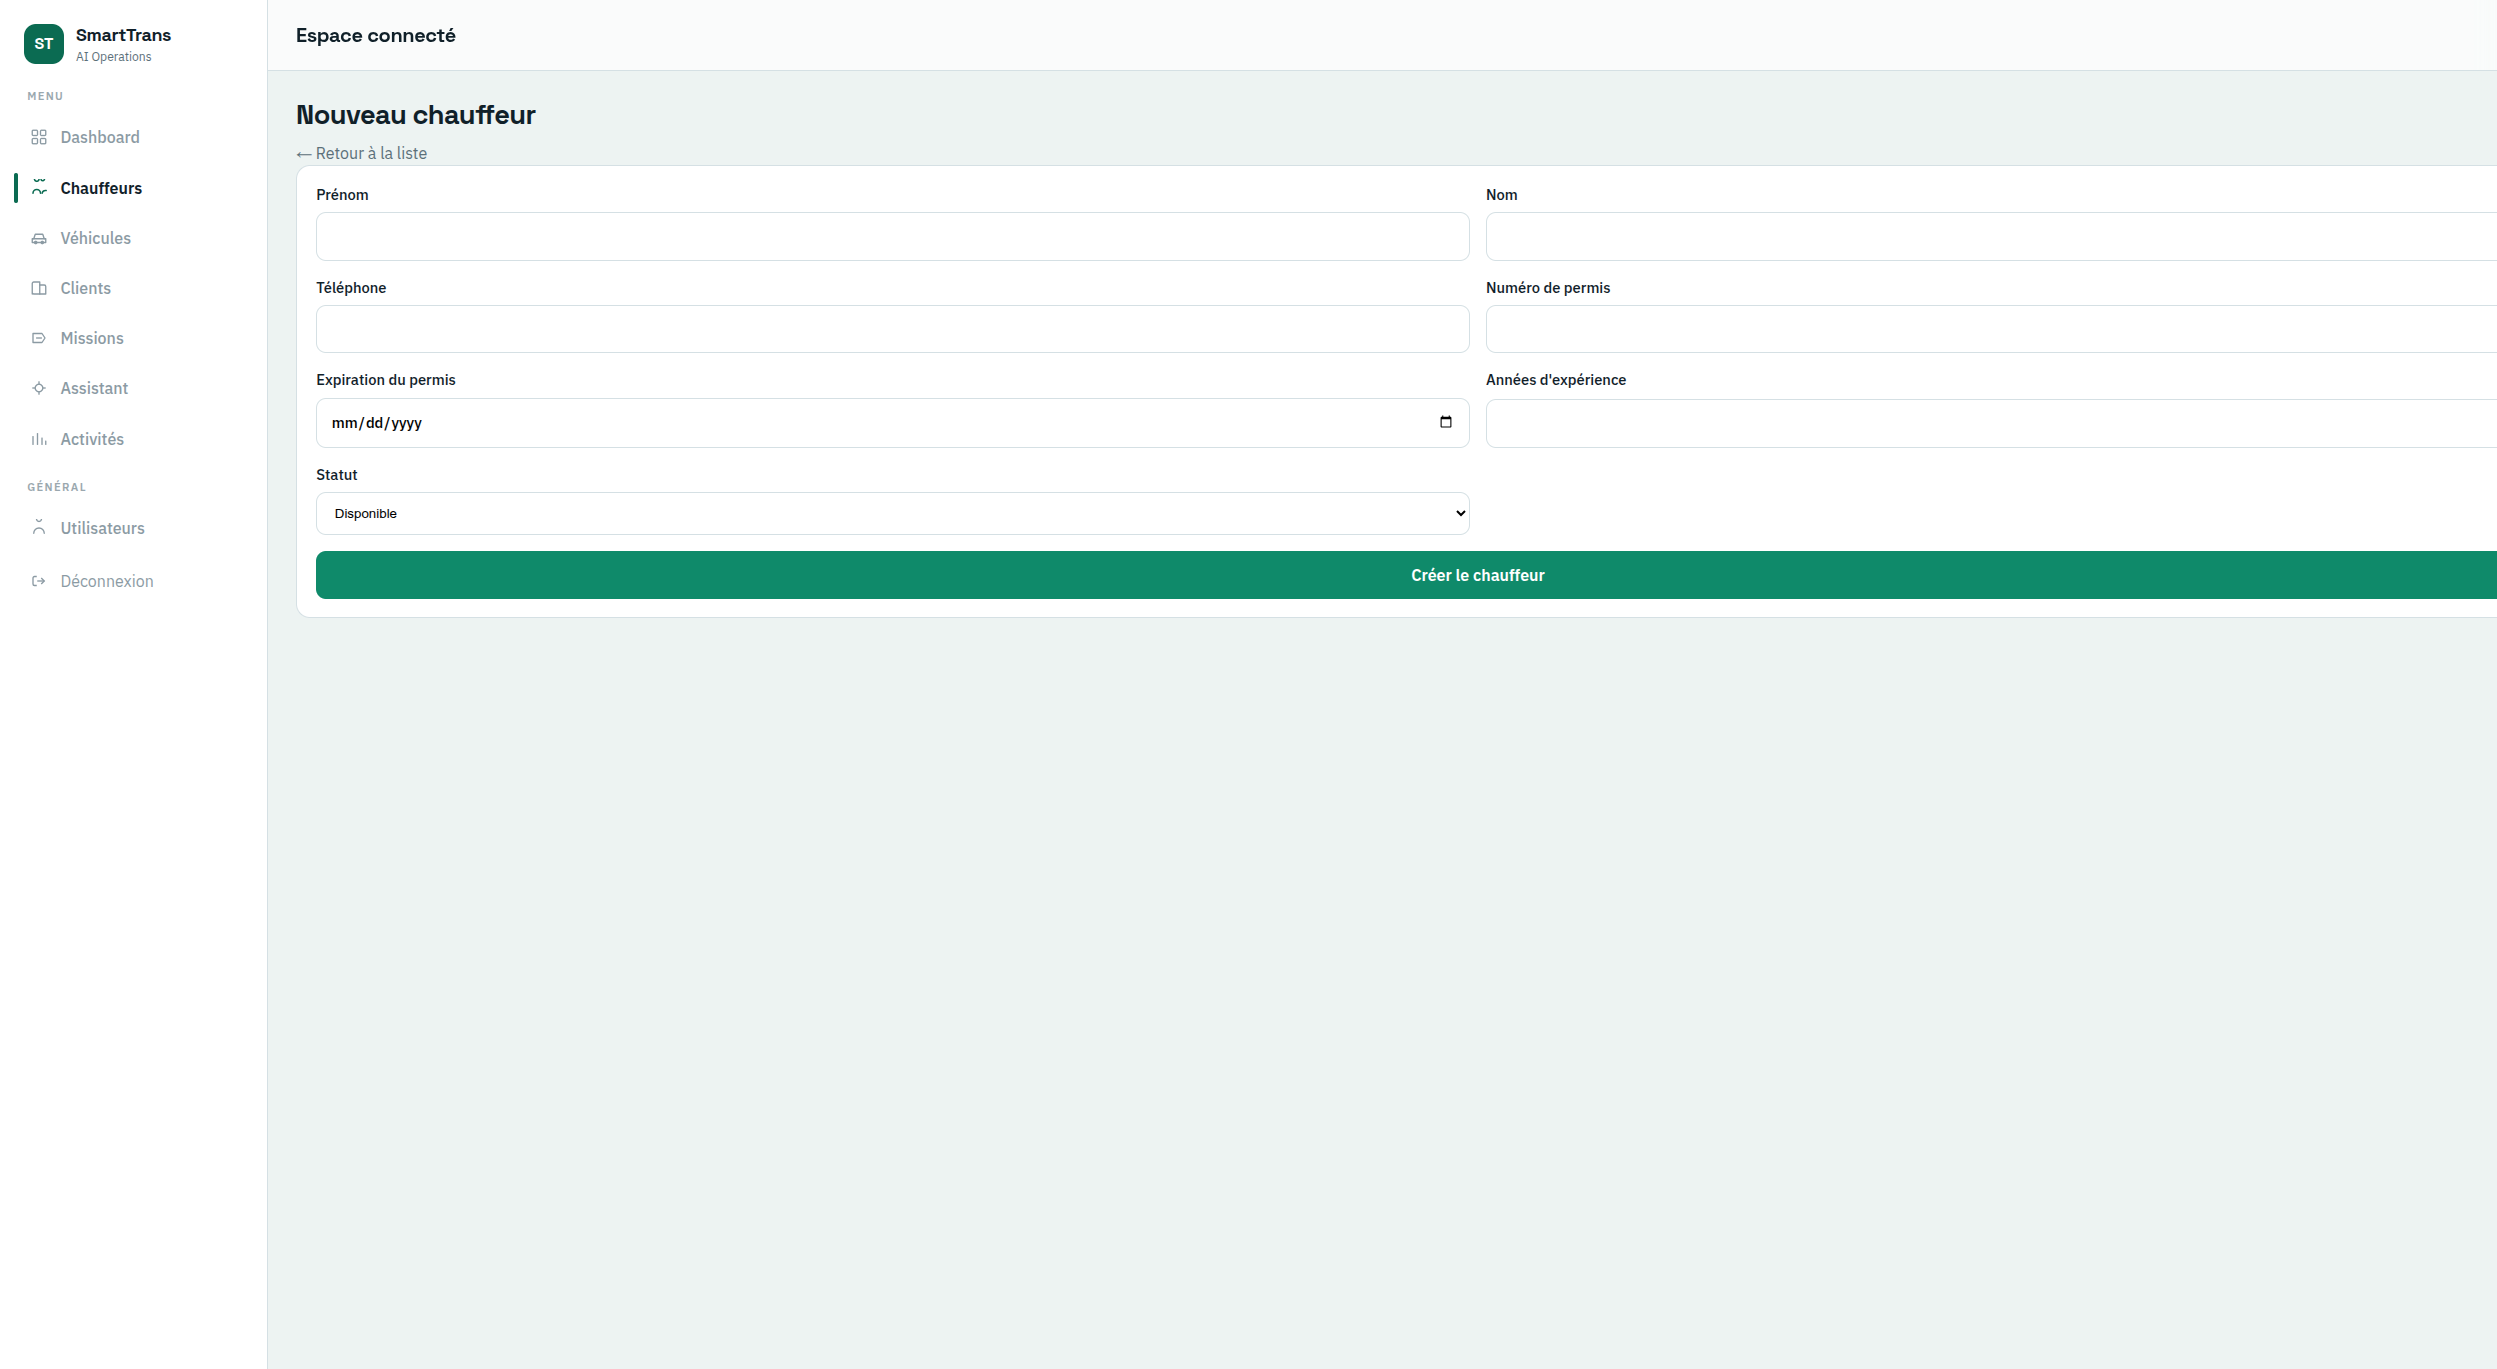
\includegraphics[width=0.88\textwidth,keepaspectratio]{ui-04-chauffeur-nouveau.png}
\caption{Formulaire de création d'un chauffeur}
\label{fig:ui-drv-new}
\end{figure}

\begin{figure}[htbp]
\centering
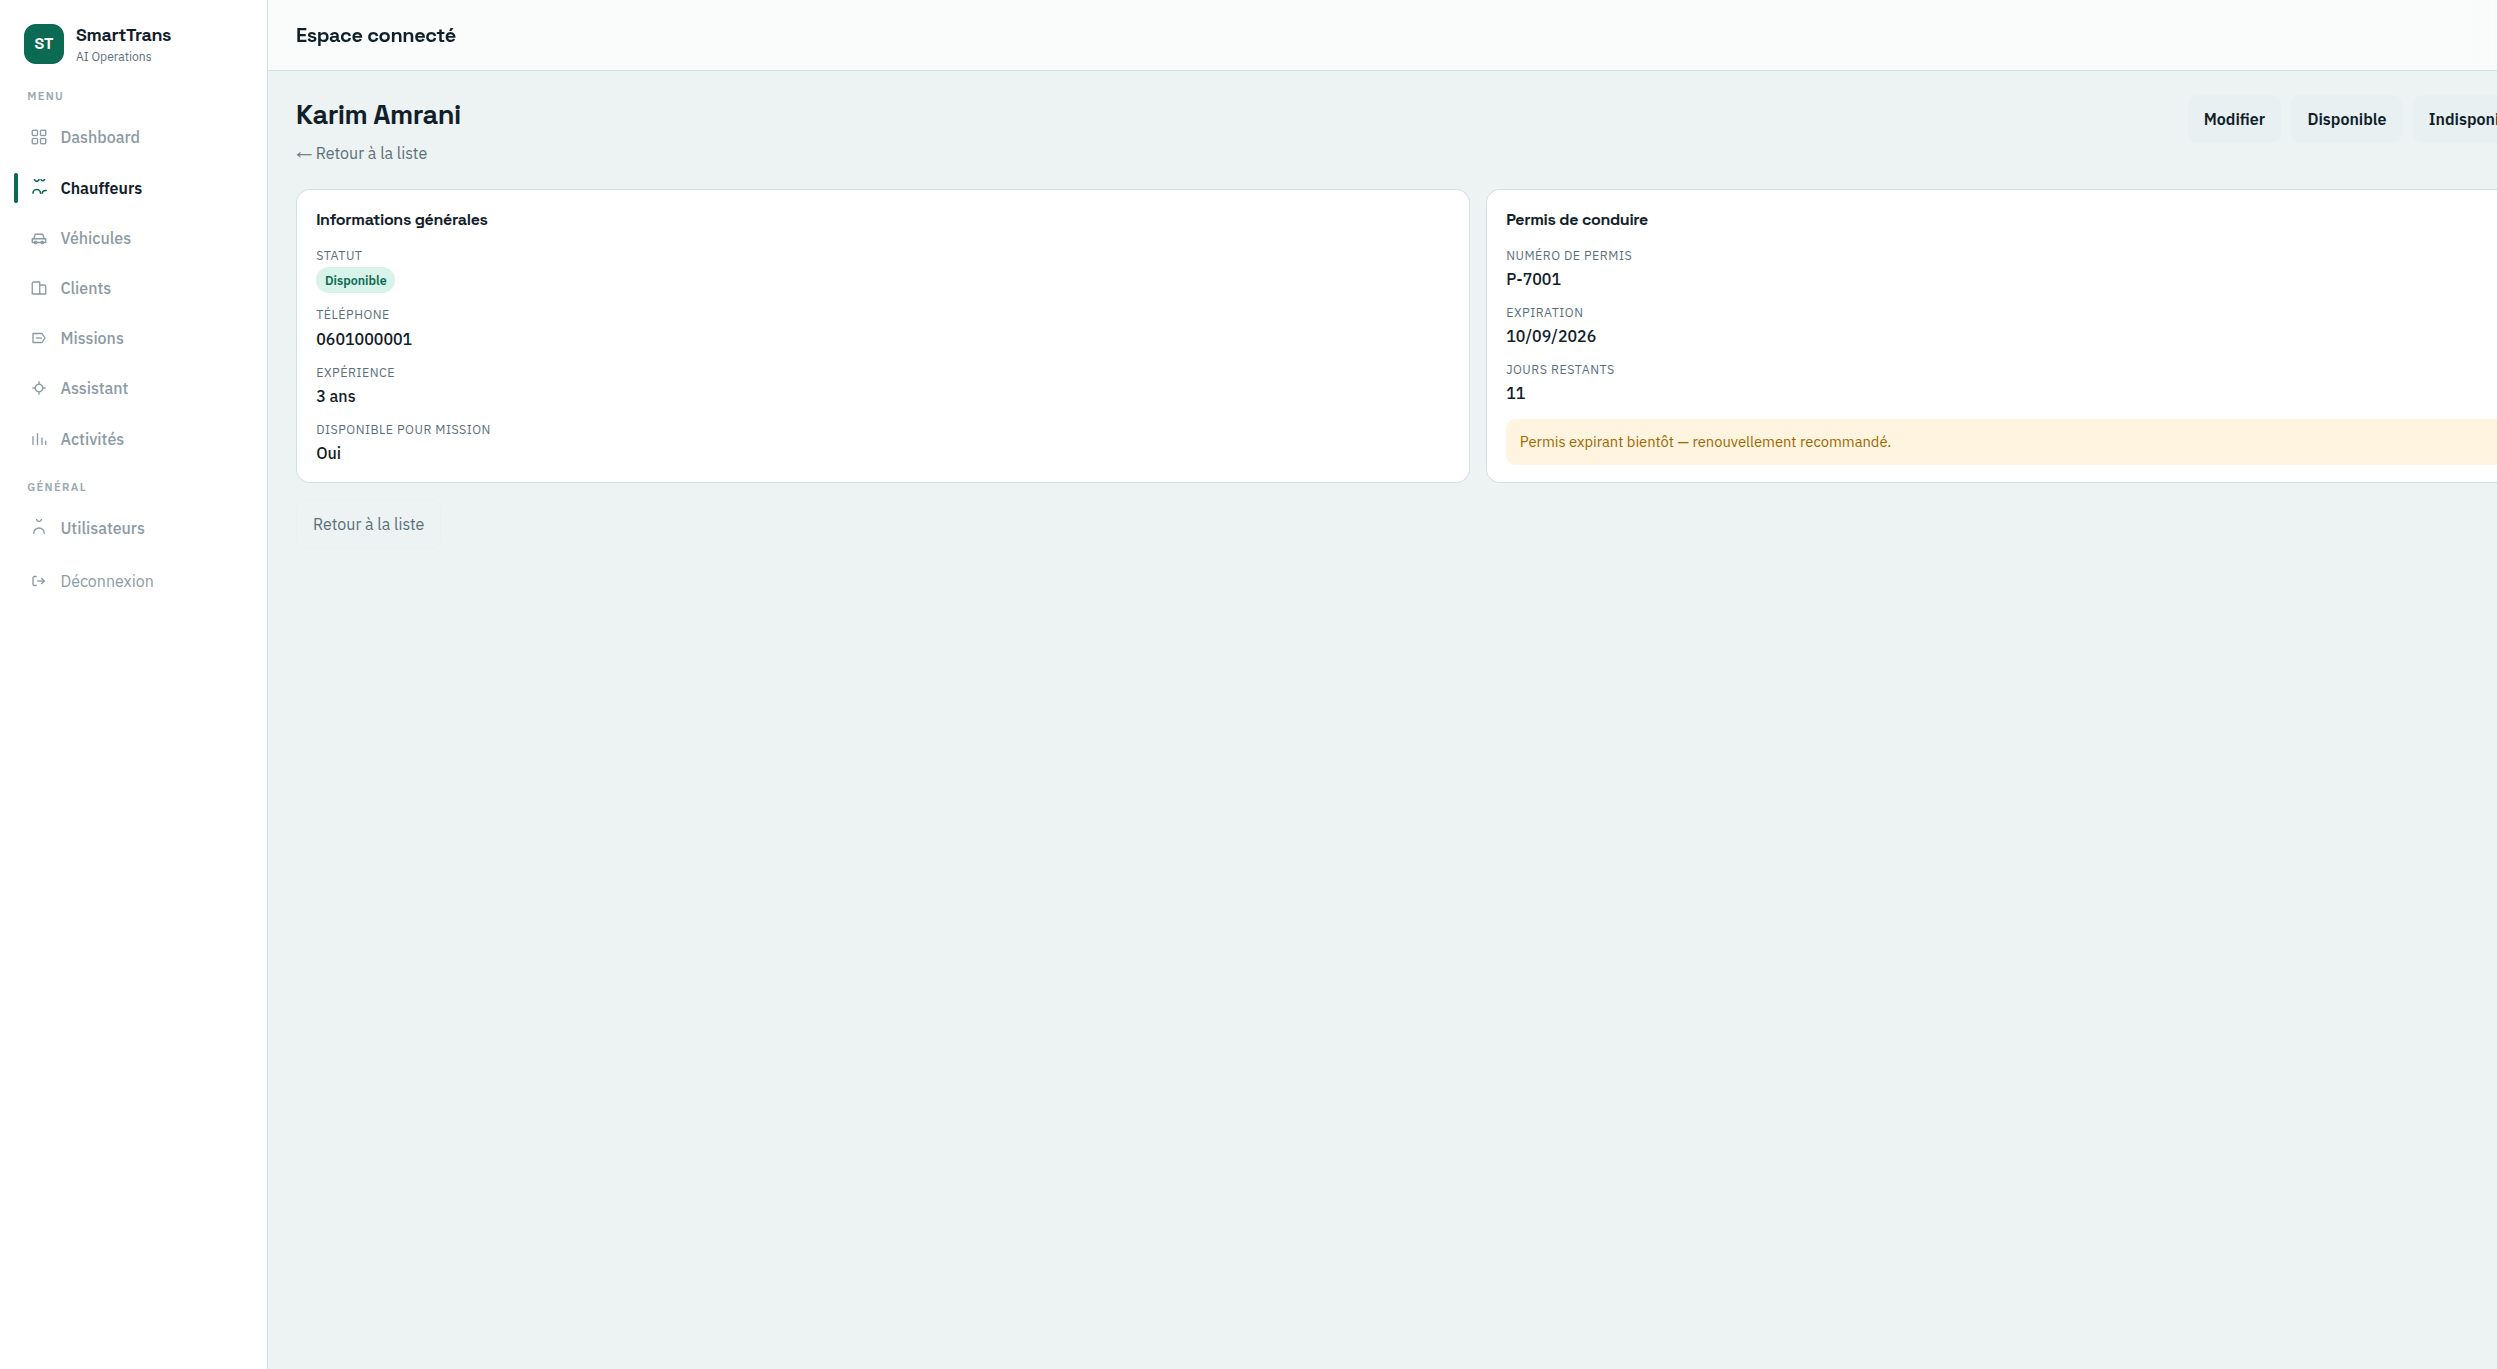
\includegraphics[width=0.88\textwidth,keepaspectratio]{ui-05-chauffeur-detail.png}
\caption{Fiche détail d'un chauffeur (alerte permis)}
\label{fig:ui-drv-det}
\end{figure}

\begin{figure}[htbp]
\centering
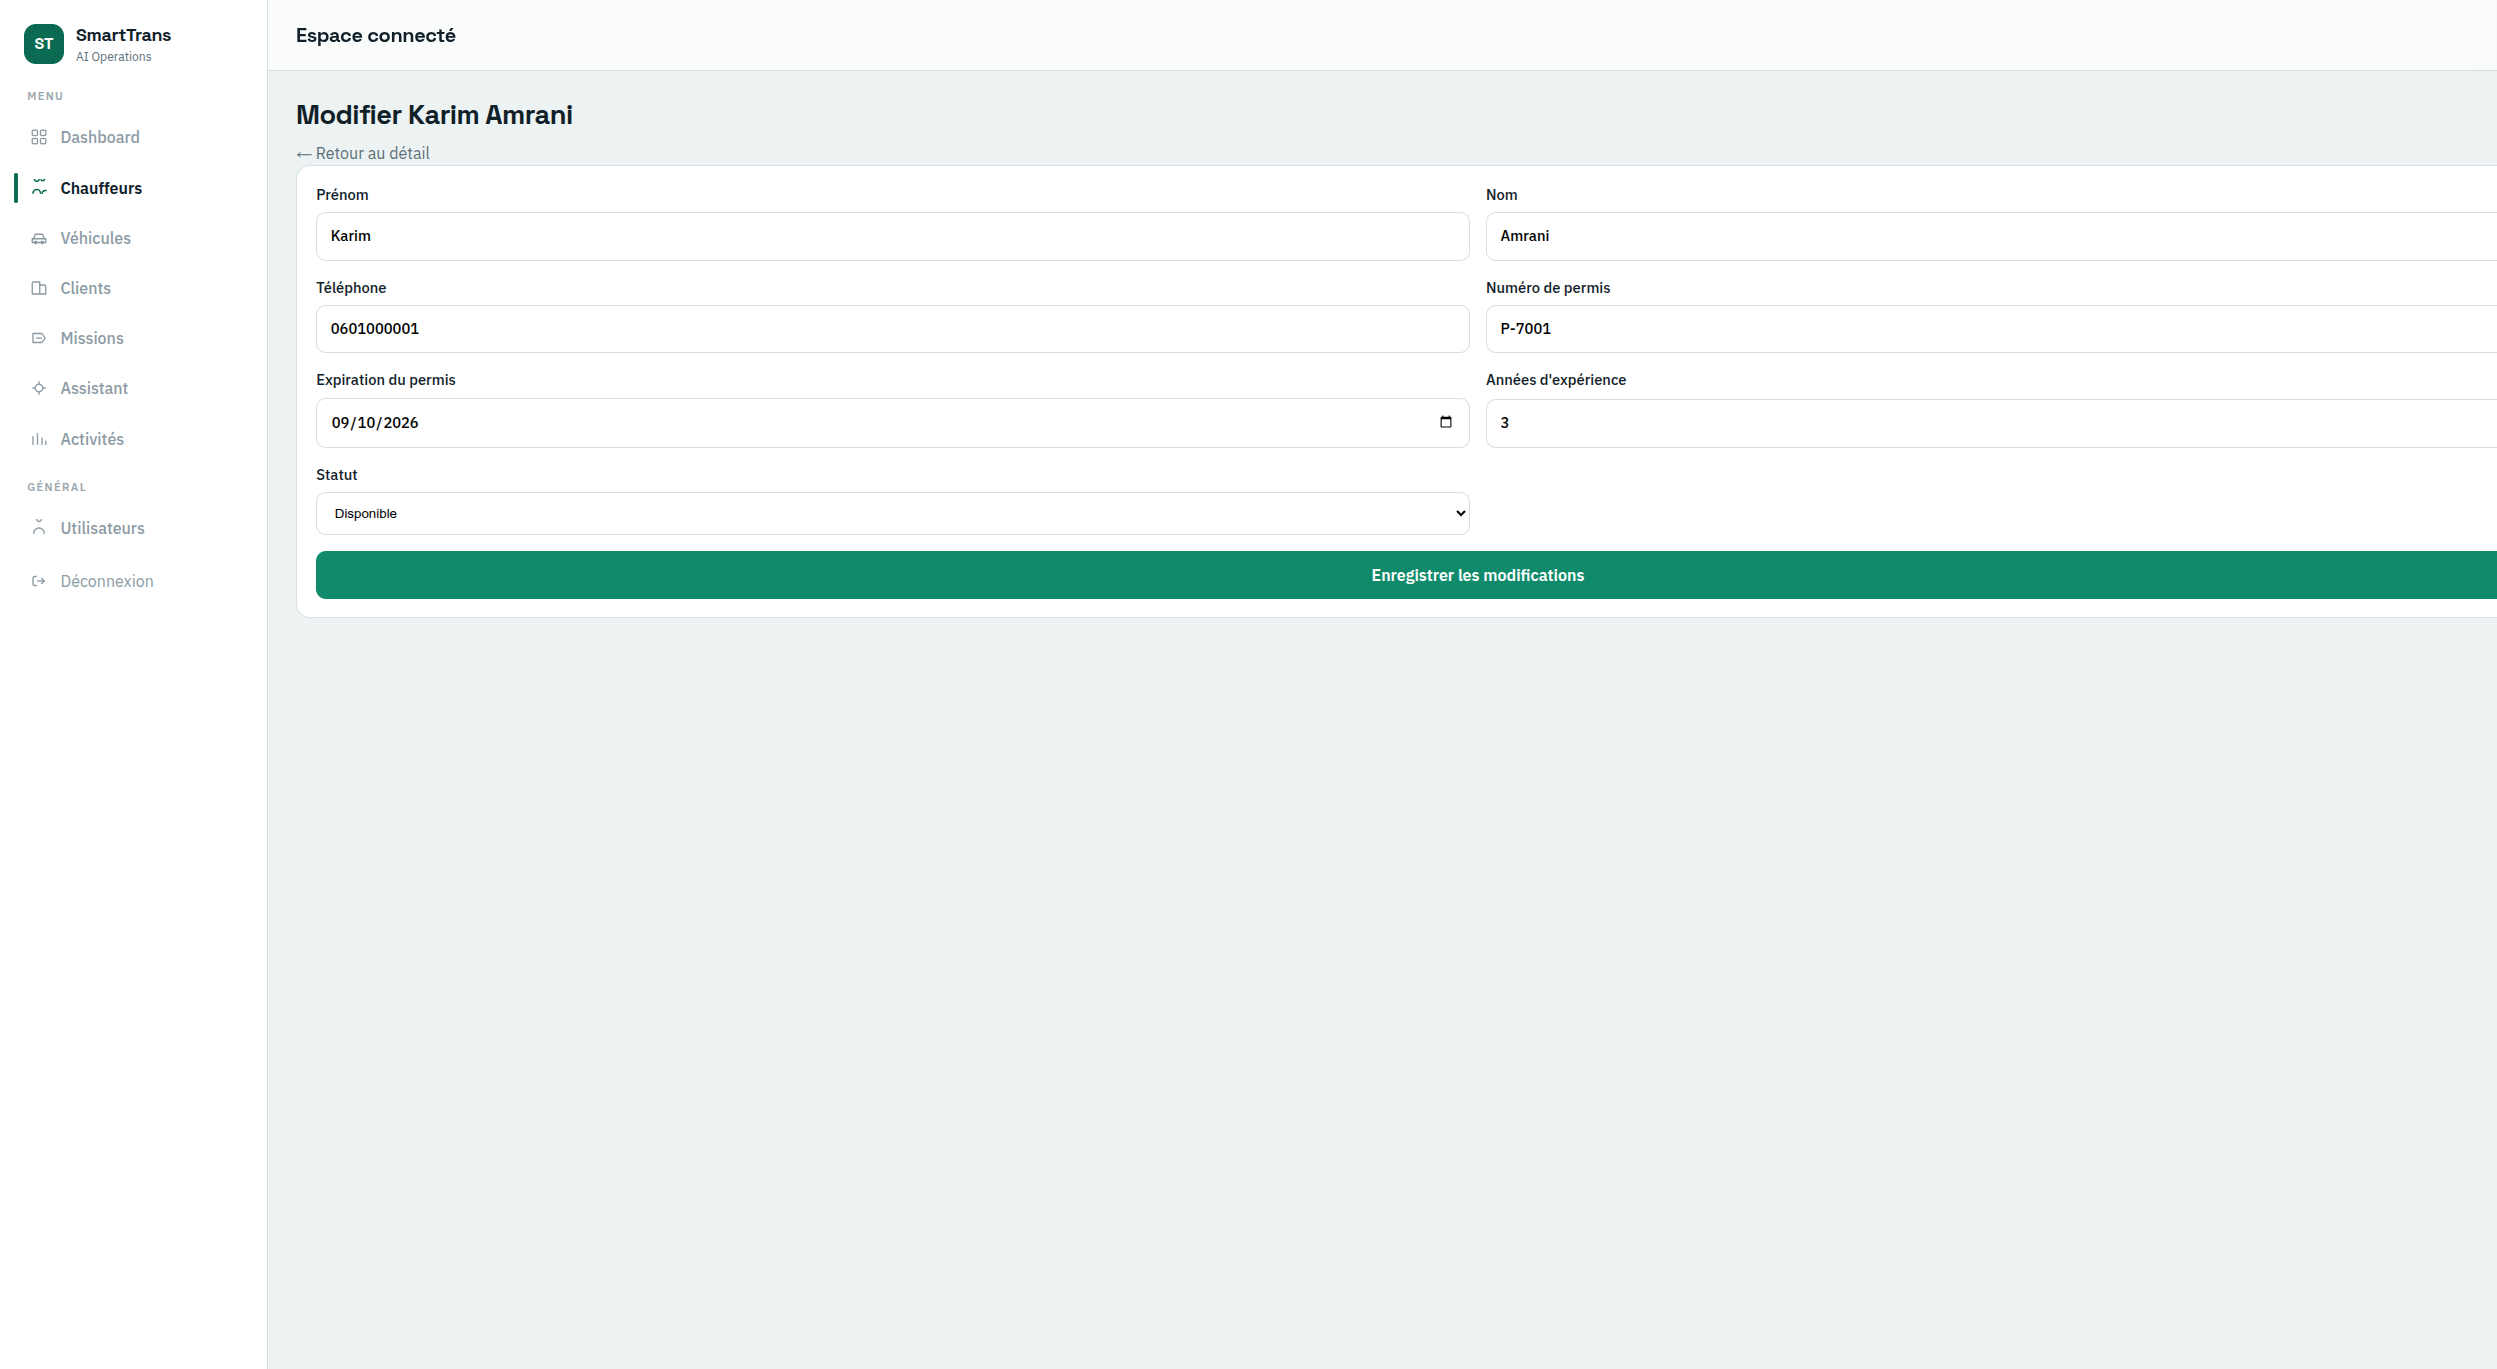
\includegraphics[width=0.88\textwidth,keepaspectratio]{ui-06-chauffeur-edit.png}
\caption{Formulaire de modification d'un chauffeur}
\label{fig:ui-drv-edit}
\end{figure}

\section{Gestion des véhicules}

La liste (figure~\ref{fig:ui-veh-list}) suit immatriculation, type, kilométrage, dates d'assurance et de visite technique, et statut d'exploitation. Le formulaire de création (figure~\ref{fig:ui-veh-new}) et la fiche détail (figure~\ref{fig:ui-veh-det}) reprennent ces champs, avec un indicateur de validité des documents.

\begin{figure}[htbp]
\centering
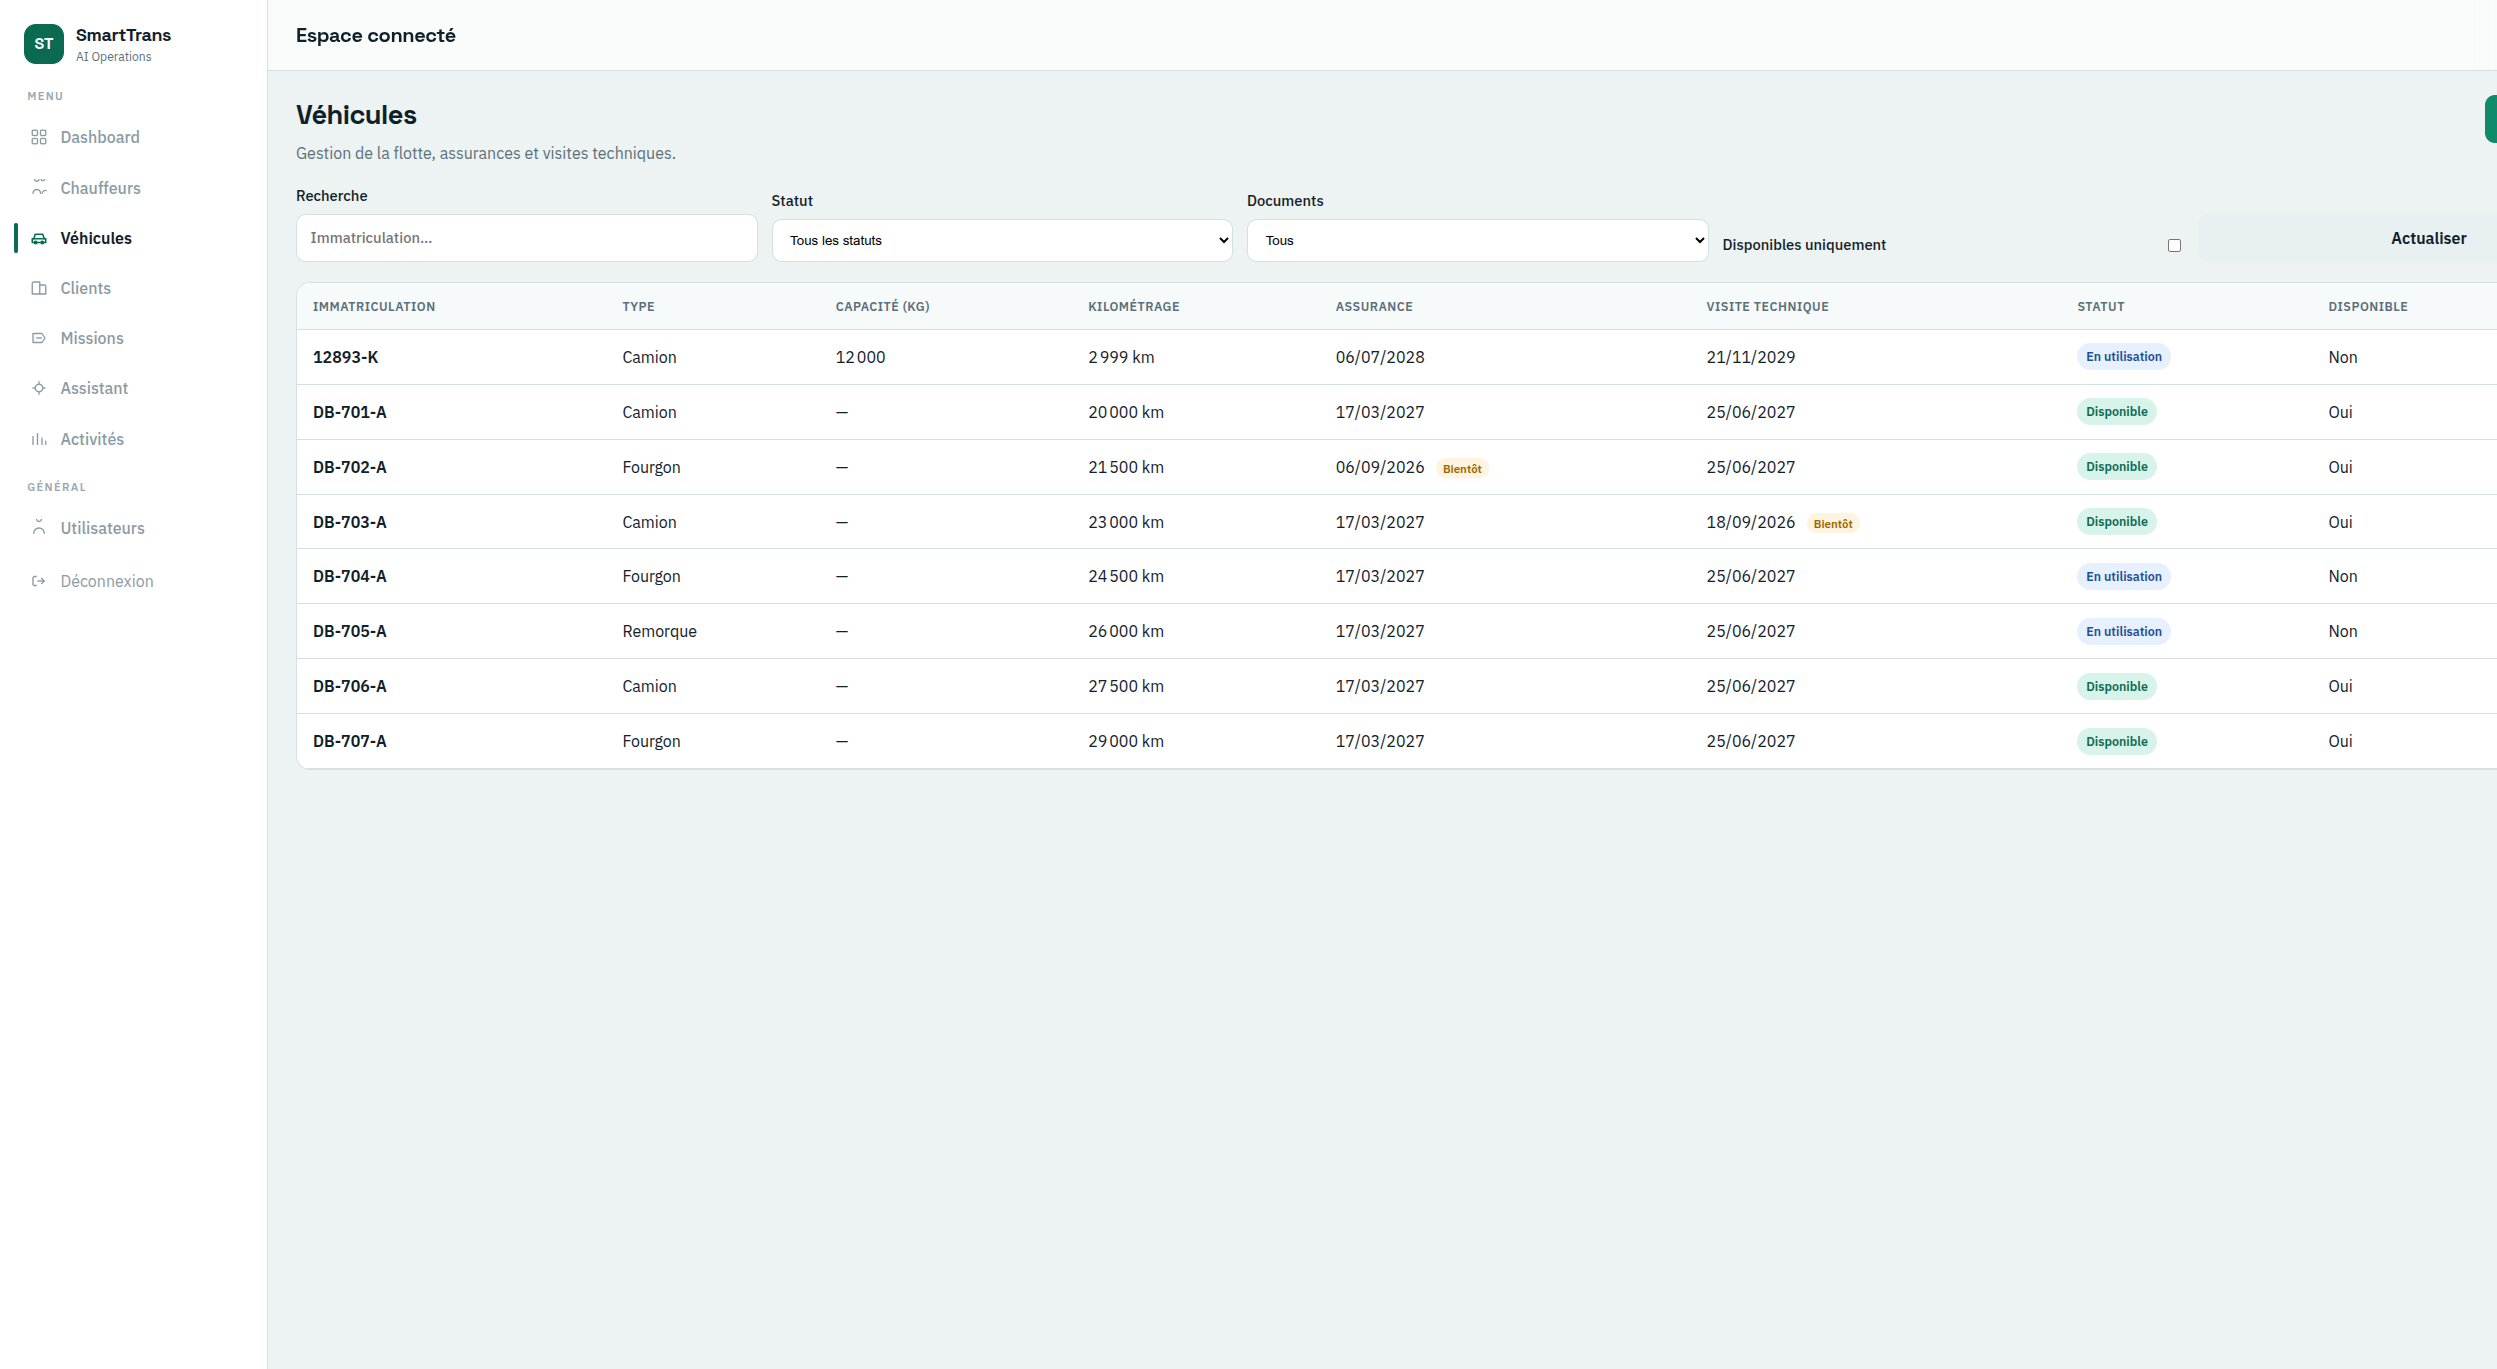
\includegraphics[width=0.95\textwidth,keepaspectratio]{ui-07-vehicules.png}
\caption{Liste des véhicules}
\label{fig:ui-veh-list}
\end{figure}

\begin{figure}[htbp]
\centering
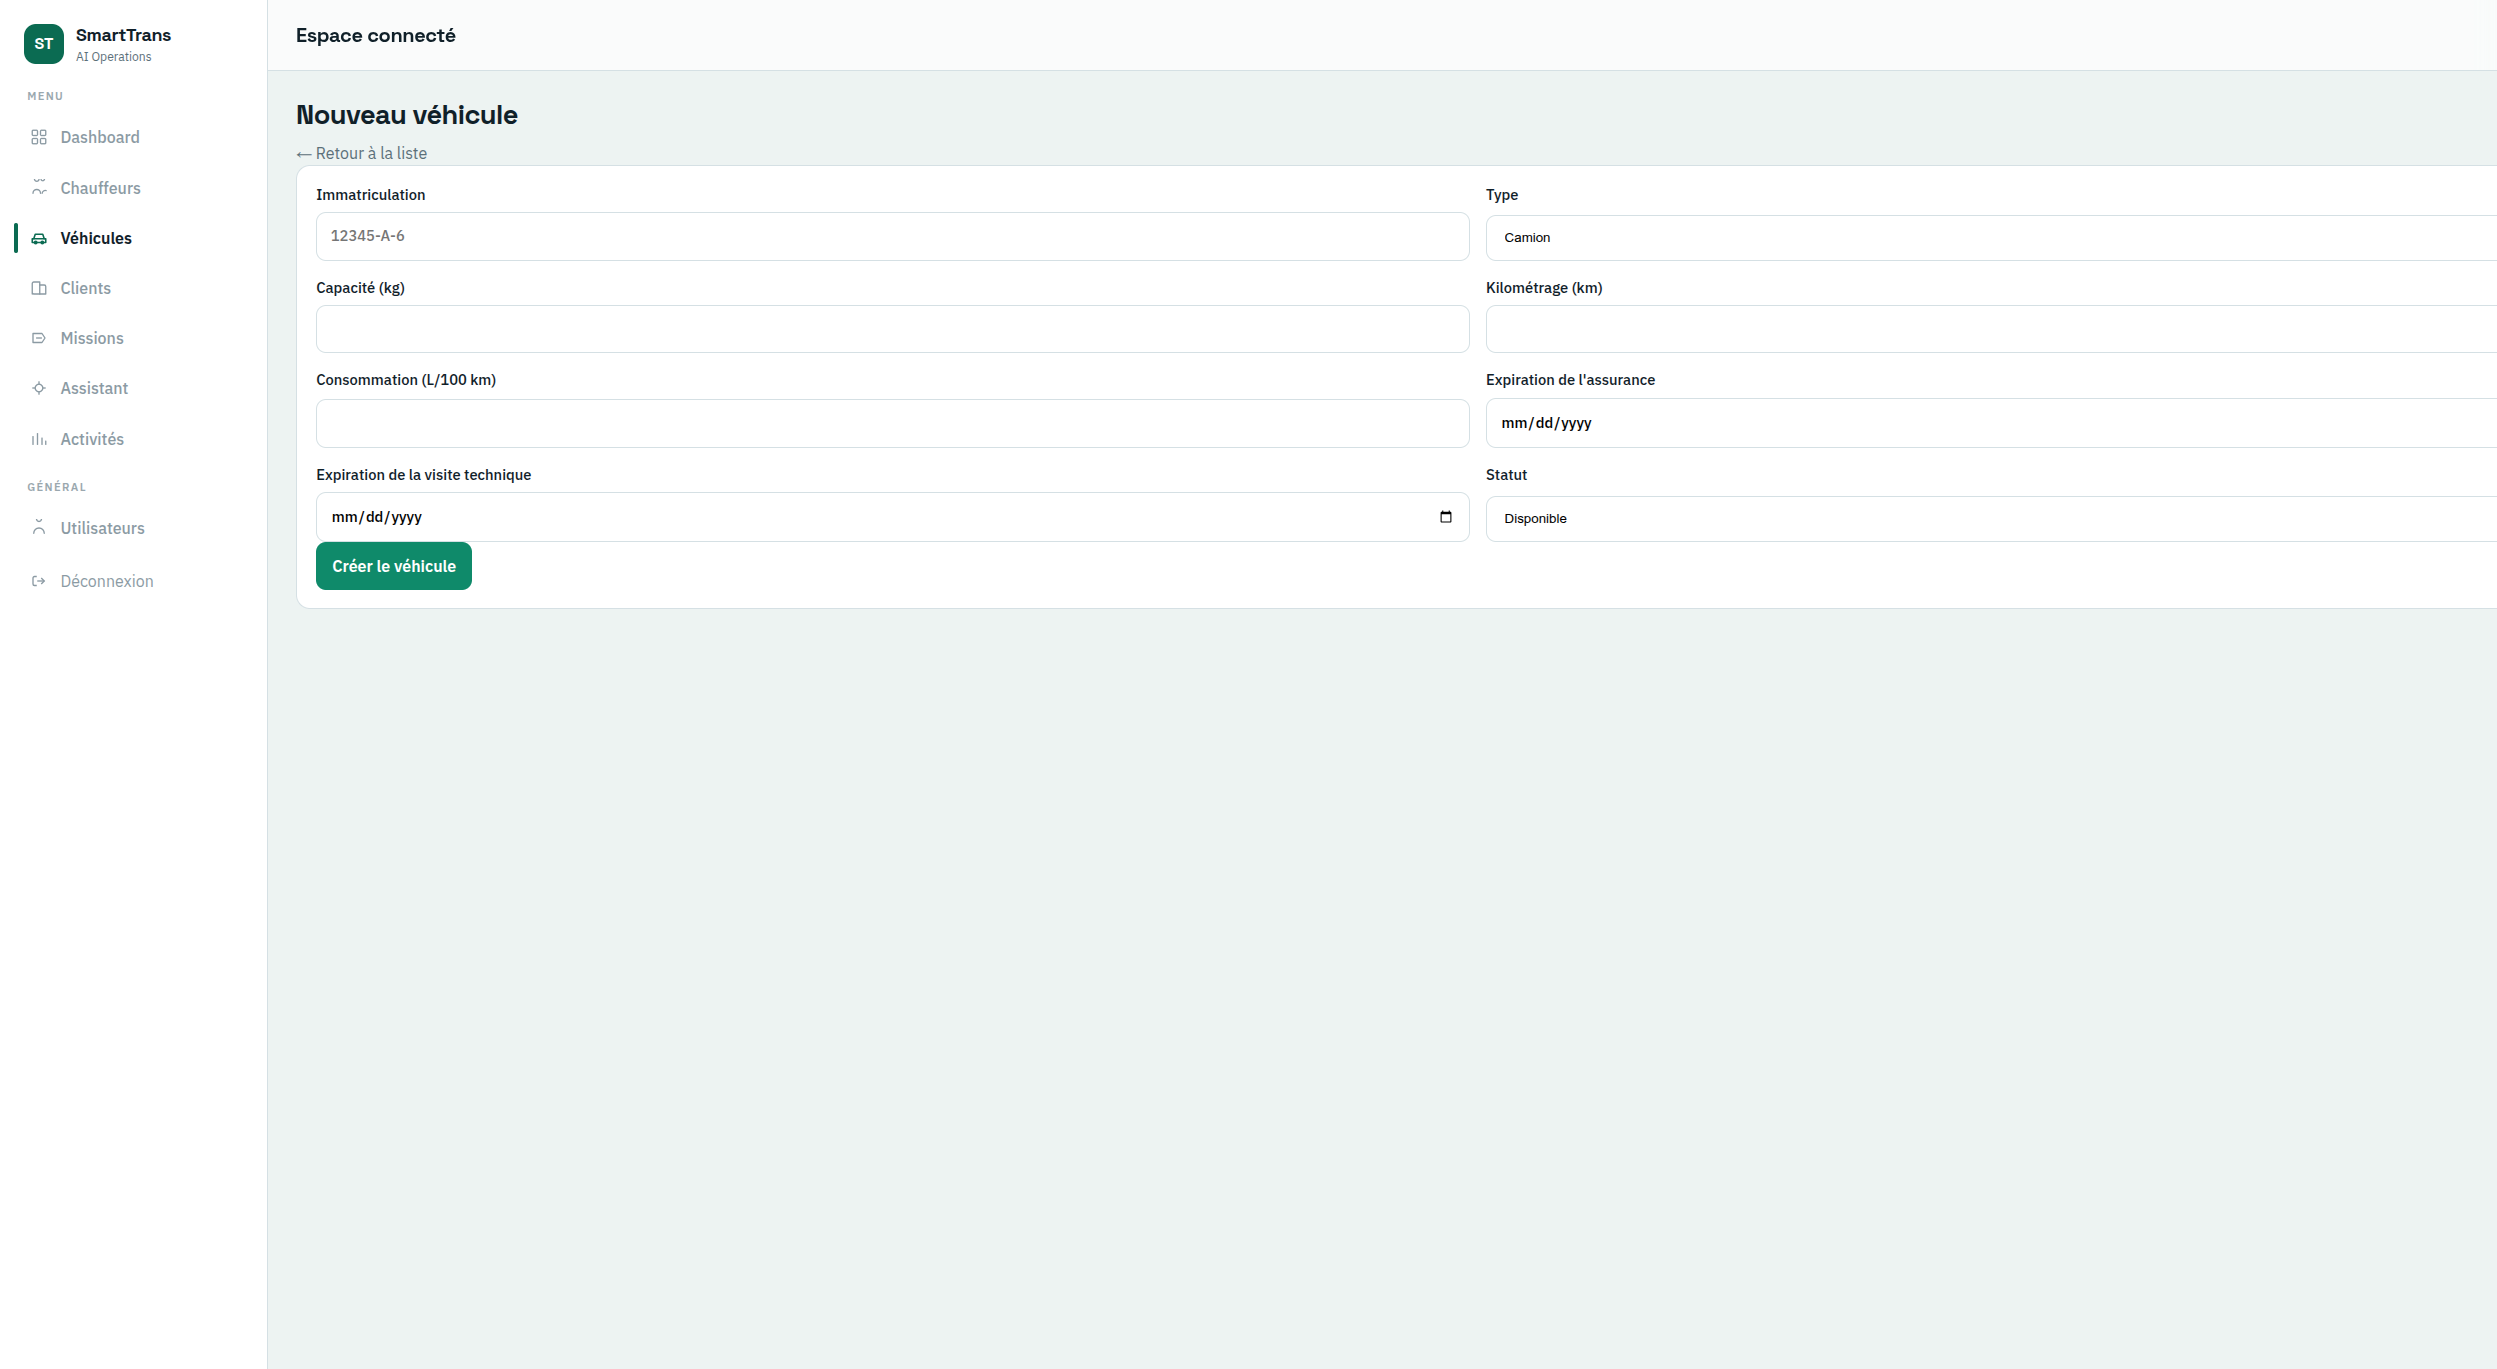
\includegraphics[width=0.88\textwidth,keepaspectratio]{ui-08-vehicule-nouveau.png}
\caption{Formulaire de création d'un véhicule}
\label{fig:ui-veh-new}
\end{figure}

\begin{figure}[htbp]
\centering
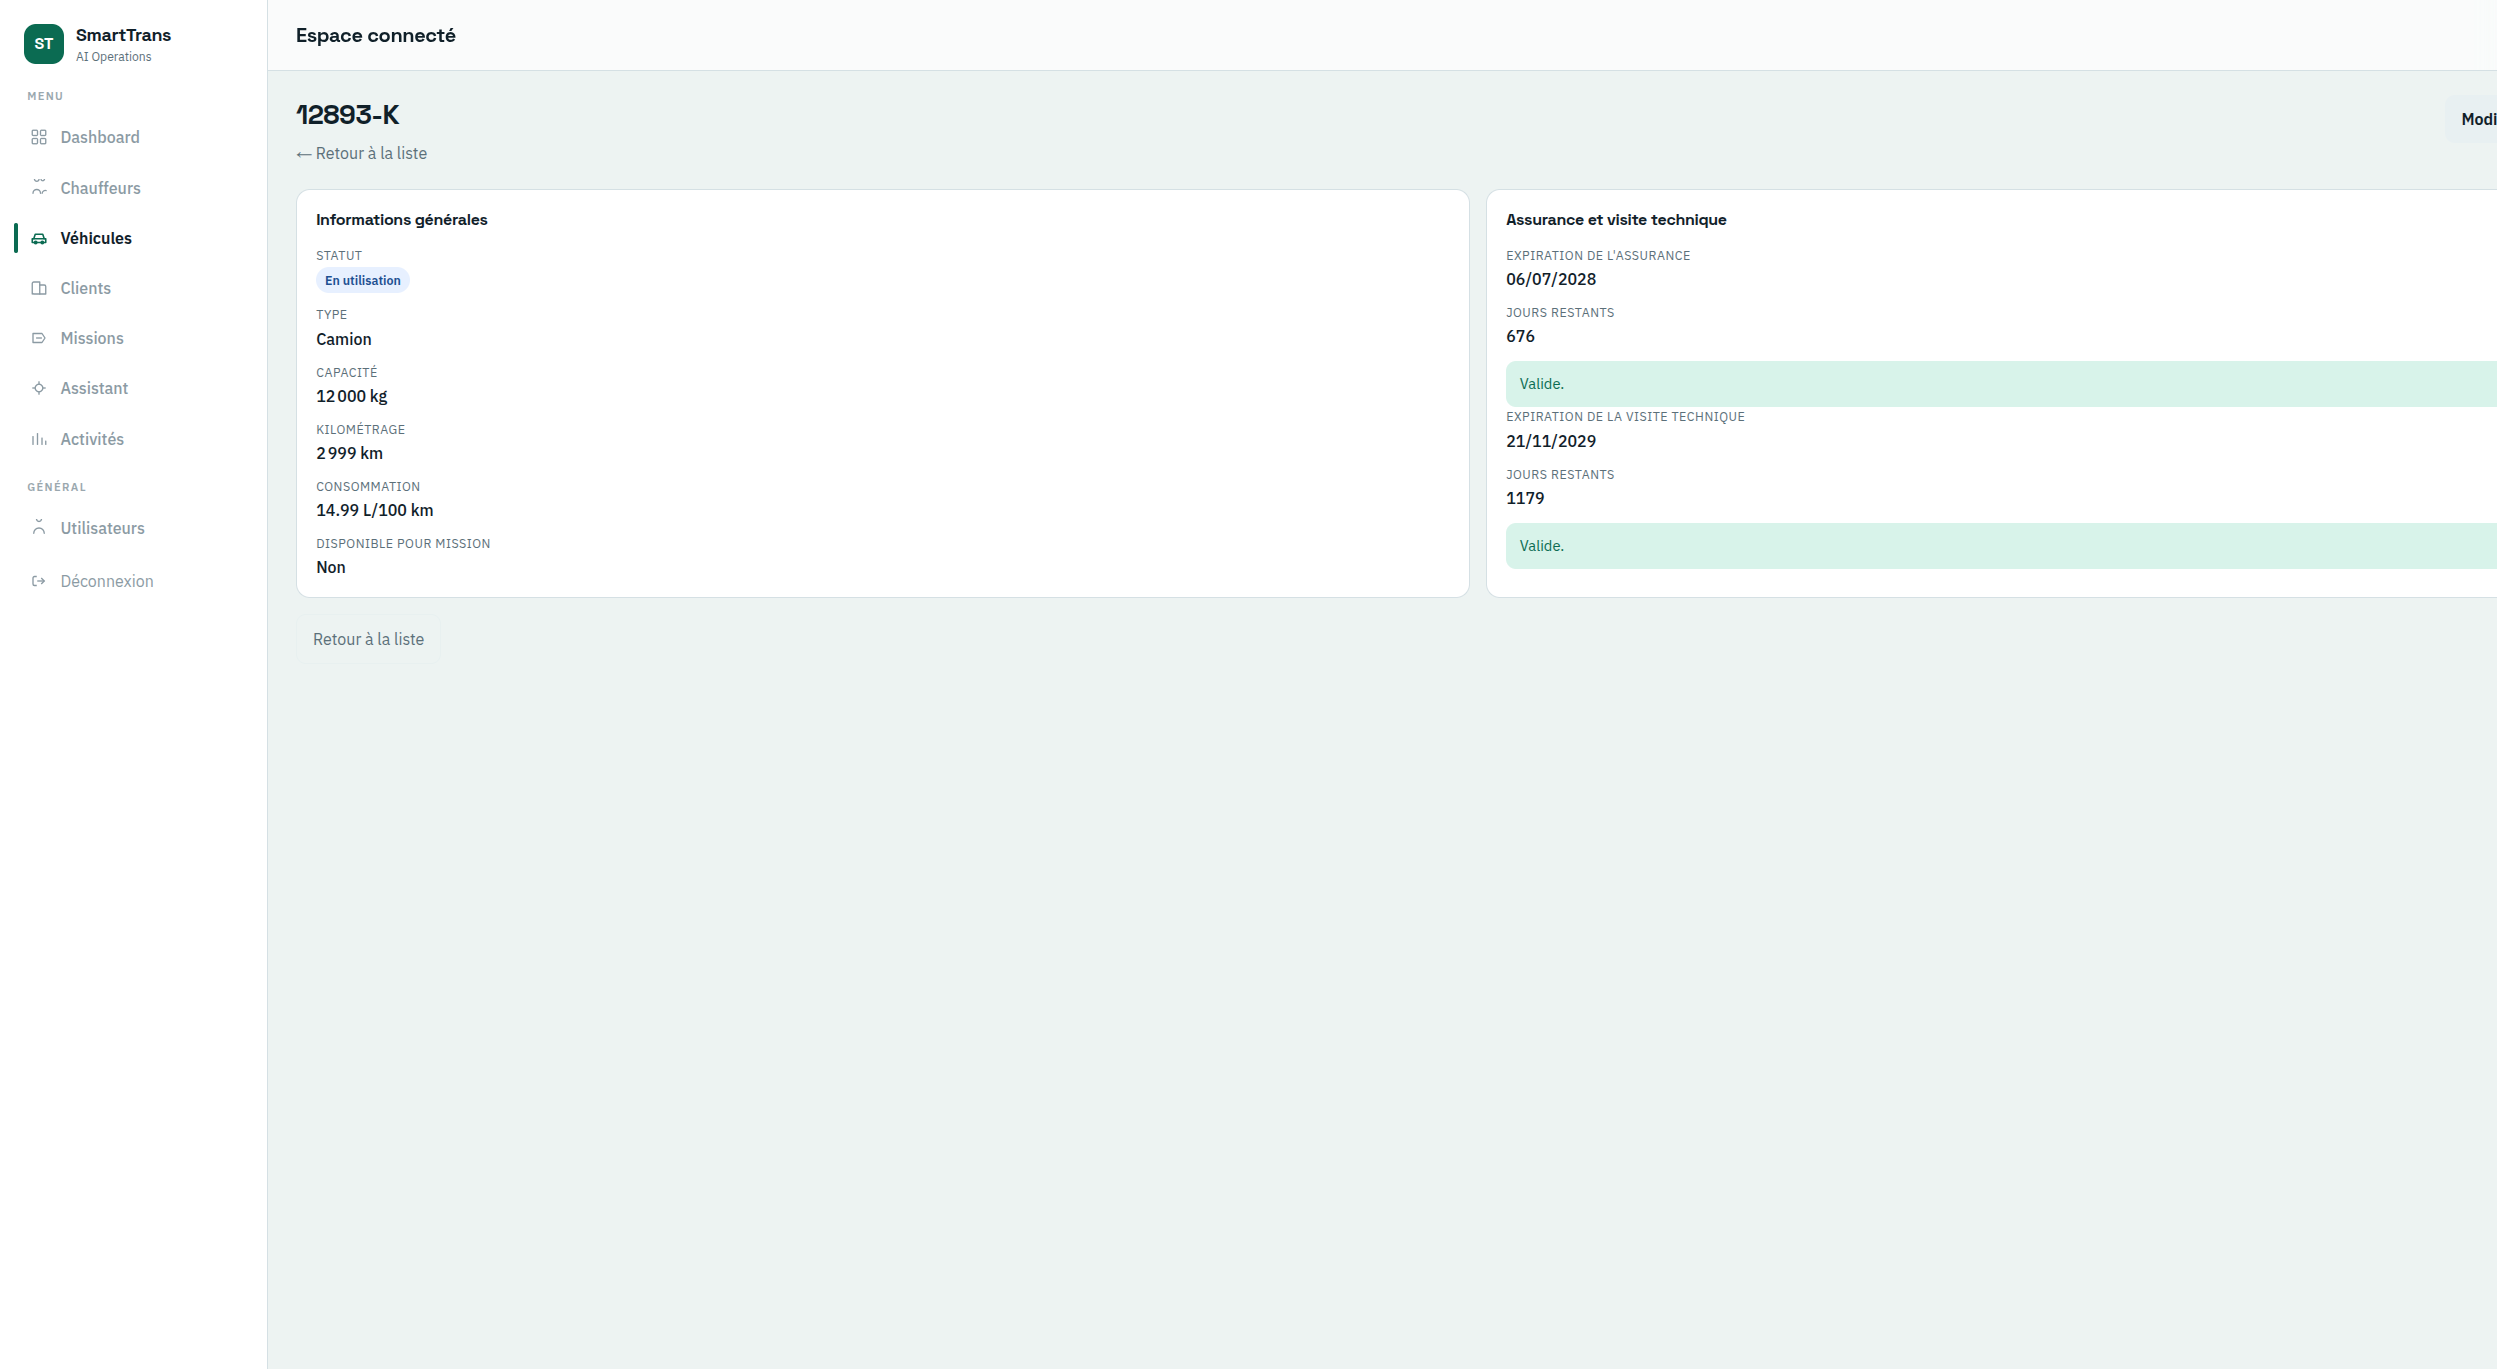
\includegraphics[width=0.88\textwidth,keepaspectratio]{ui-09-vehicule-detail.png}
\caption{Fiche détail d'un véhicule}
\label{fig:ui-veh-det}
\end{figure}

\section{Gestion des clients}

Les clients sont les entreprises destinataires des missions. La liste (figure~\ref{fig:ui-cli-list}) affiche le nom de l'entreprise, les coordonnées et l'adresse. La création (figure~\ref{fig:ui-cli-new}) et le détail (figure~\ref{fig:ui-cli-det}) correspondent à ce référentiel, obligatoire à la planification d'une mission.

\begin{figure}[htbp]
\centering
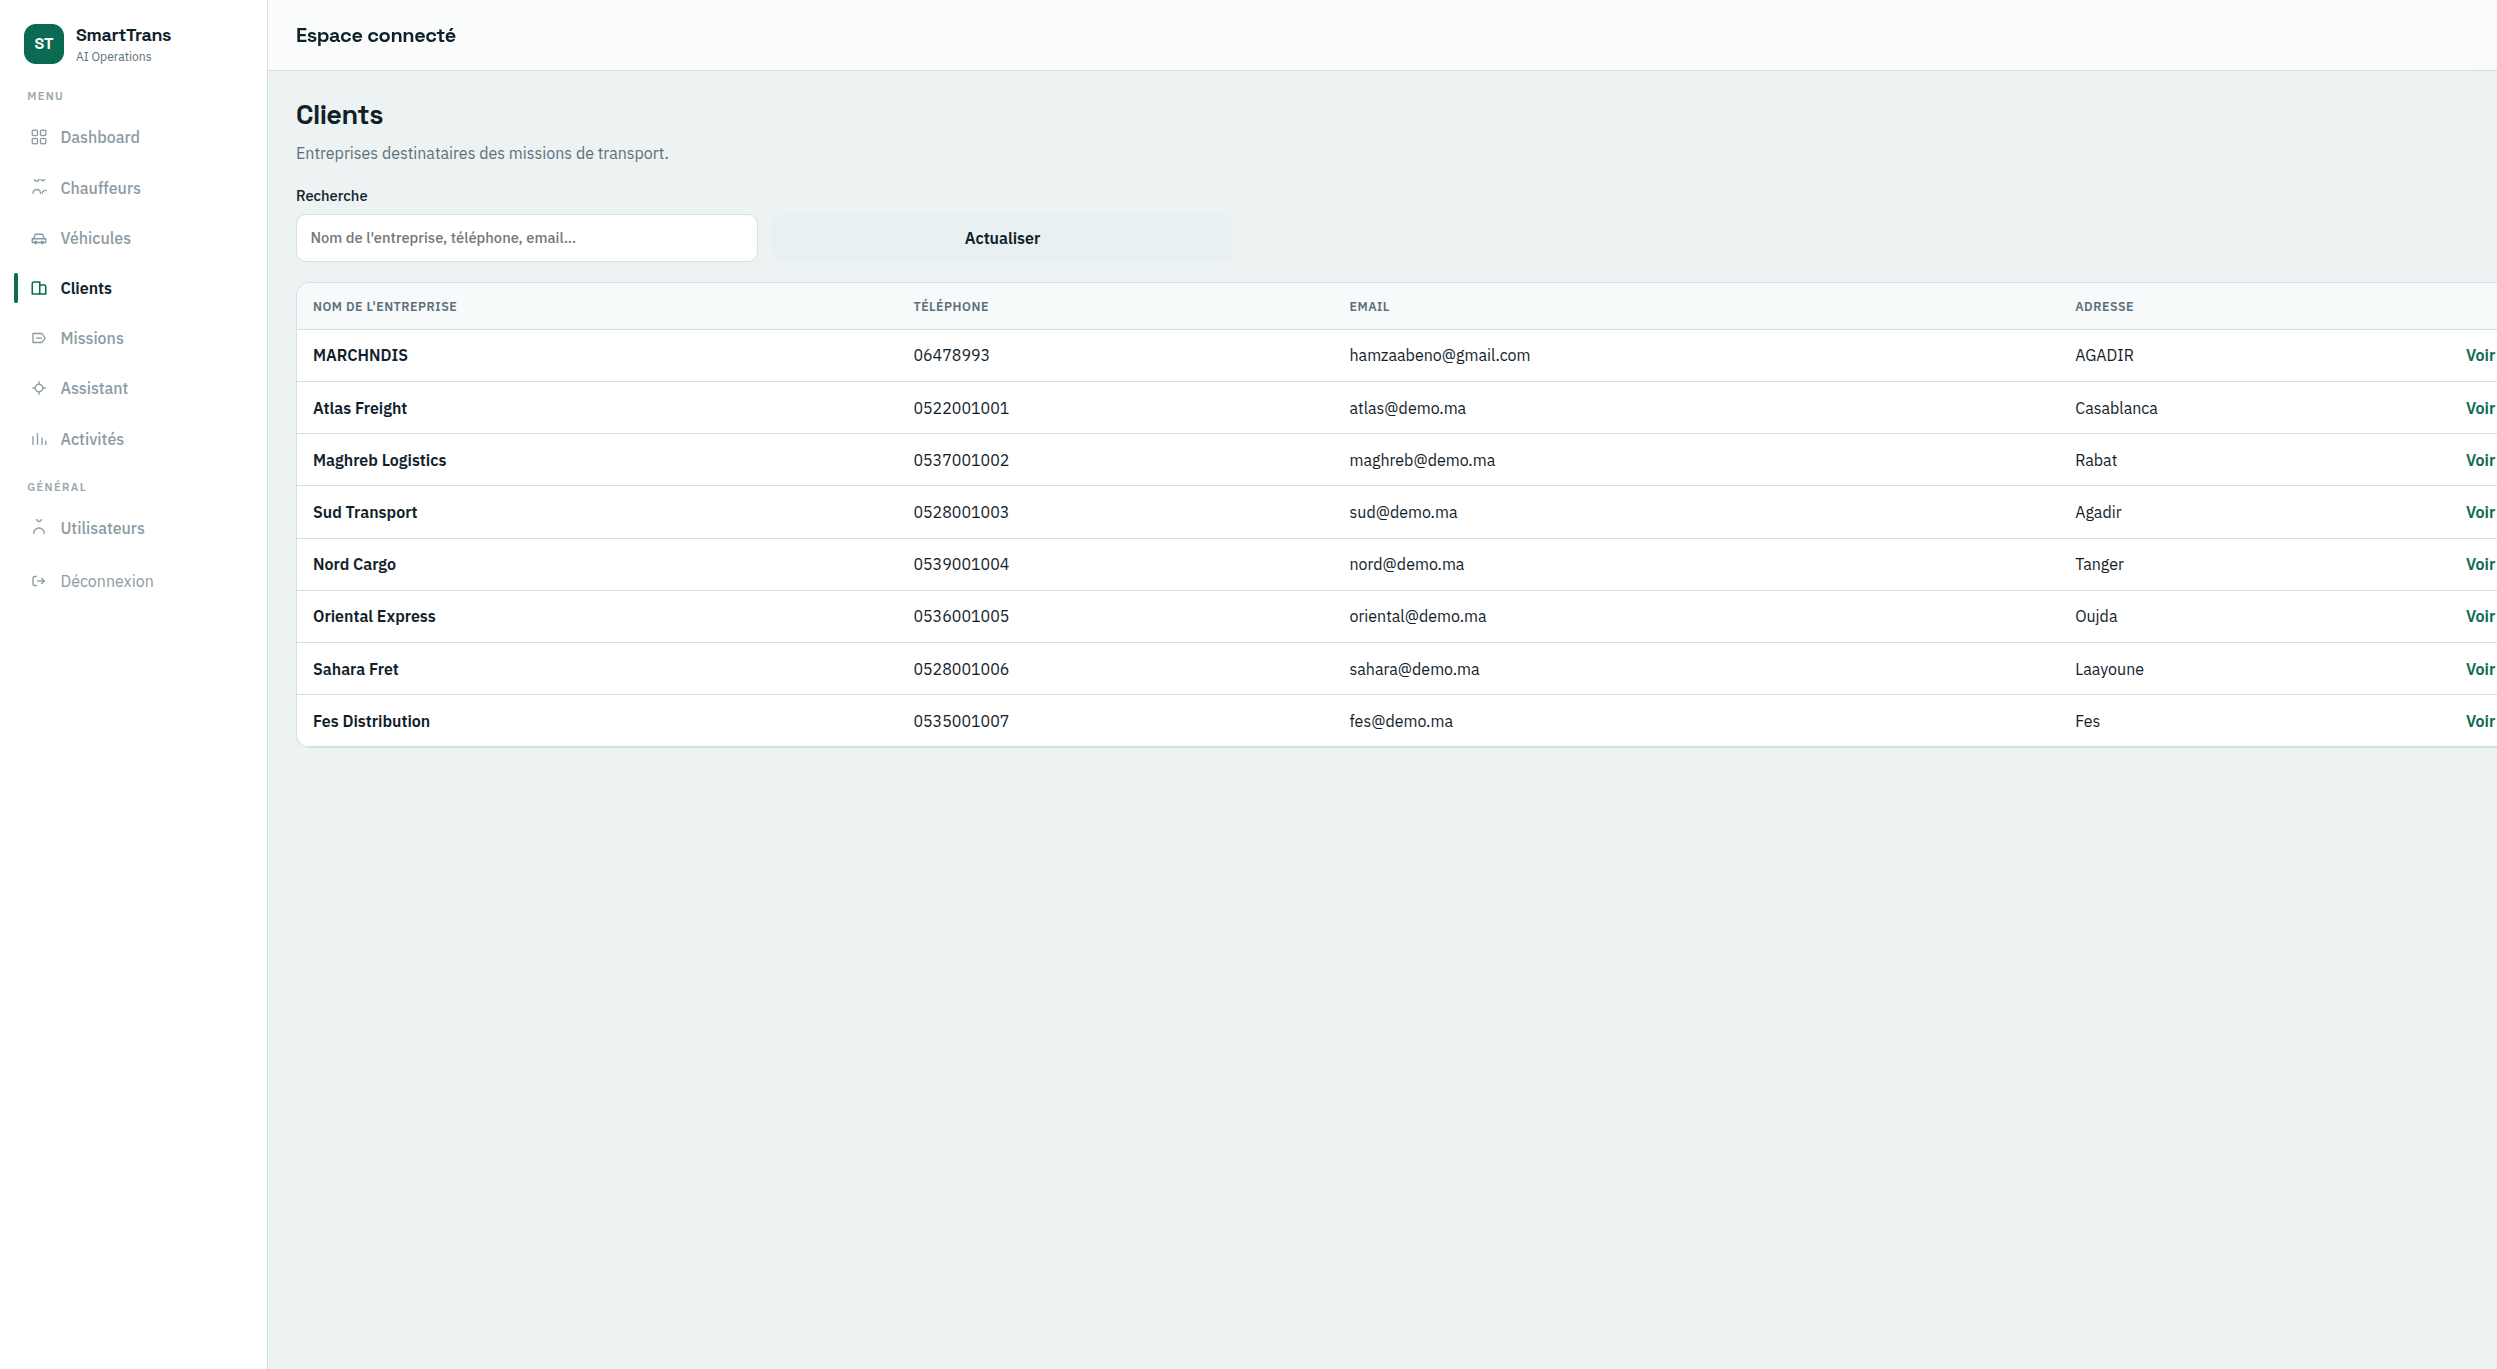
\includegraphics[width=0.95\textwidth,keepaspectratio]{ui-10-clients.png}
\caption{Liste des clients}
\label{fig:ui-cli-list}
\end{figure}

\begin{figure}[htbp]
\centering
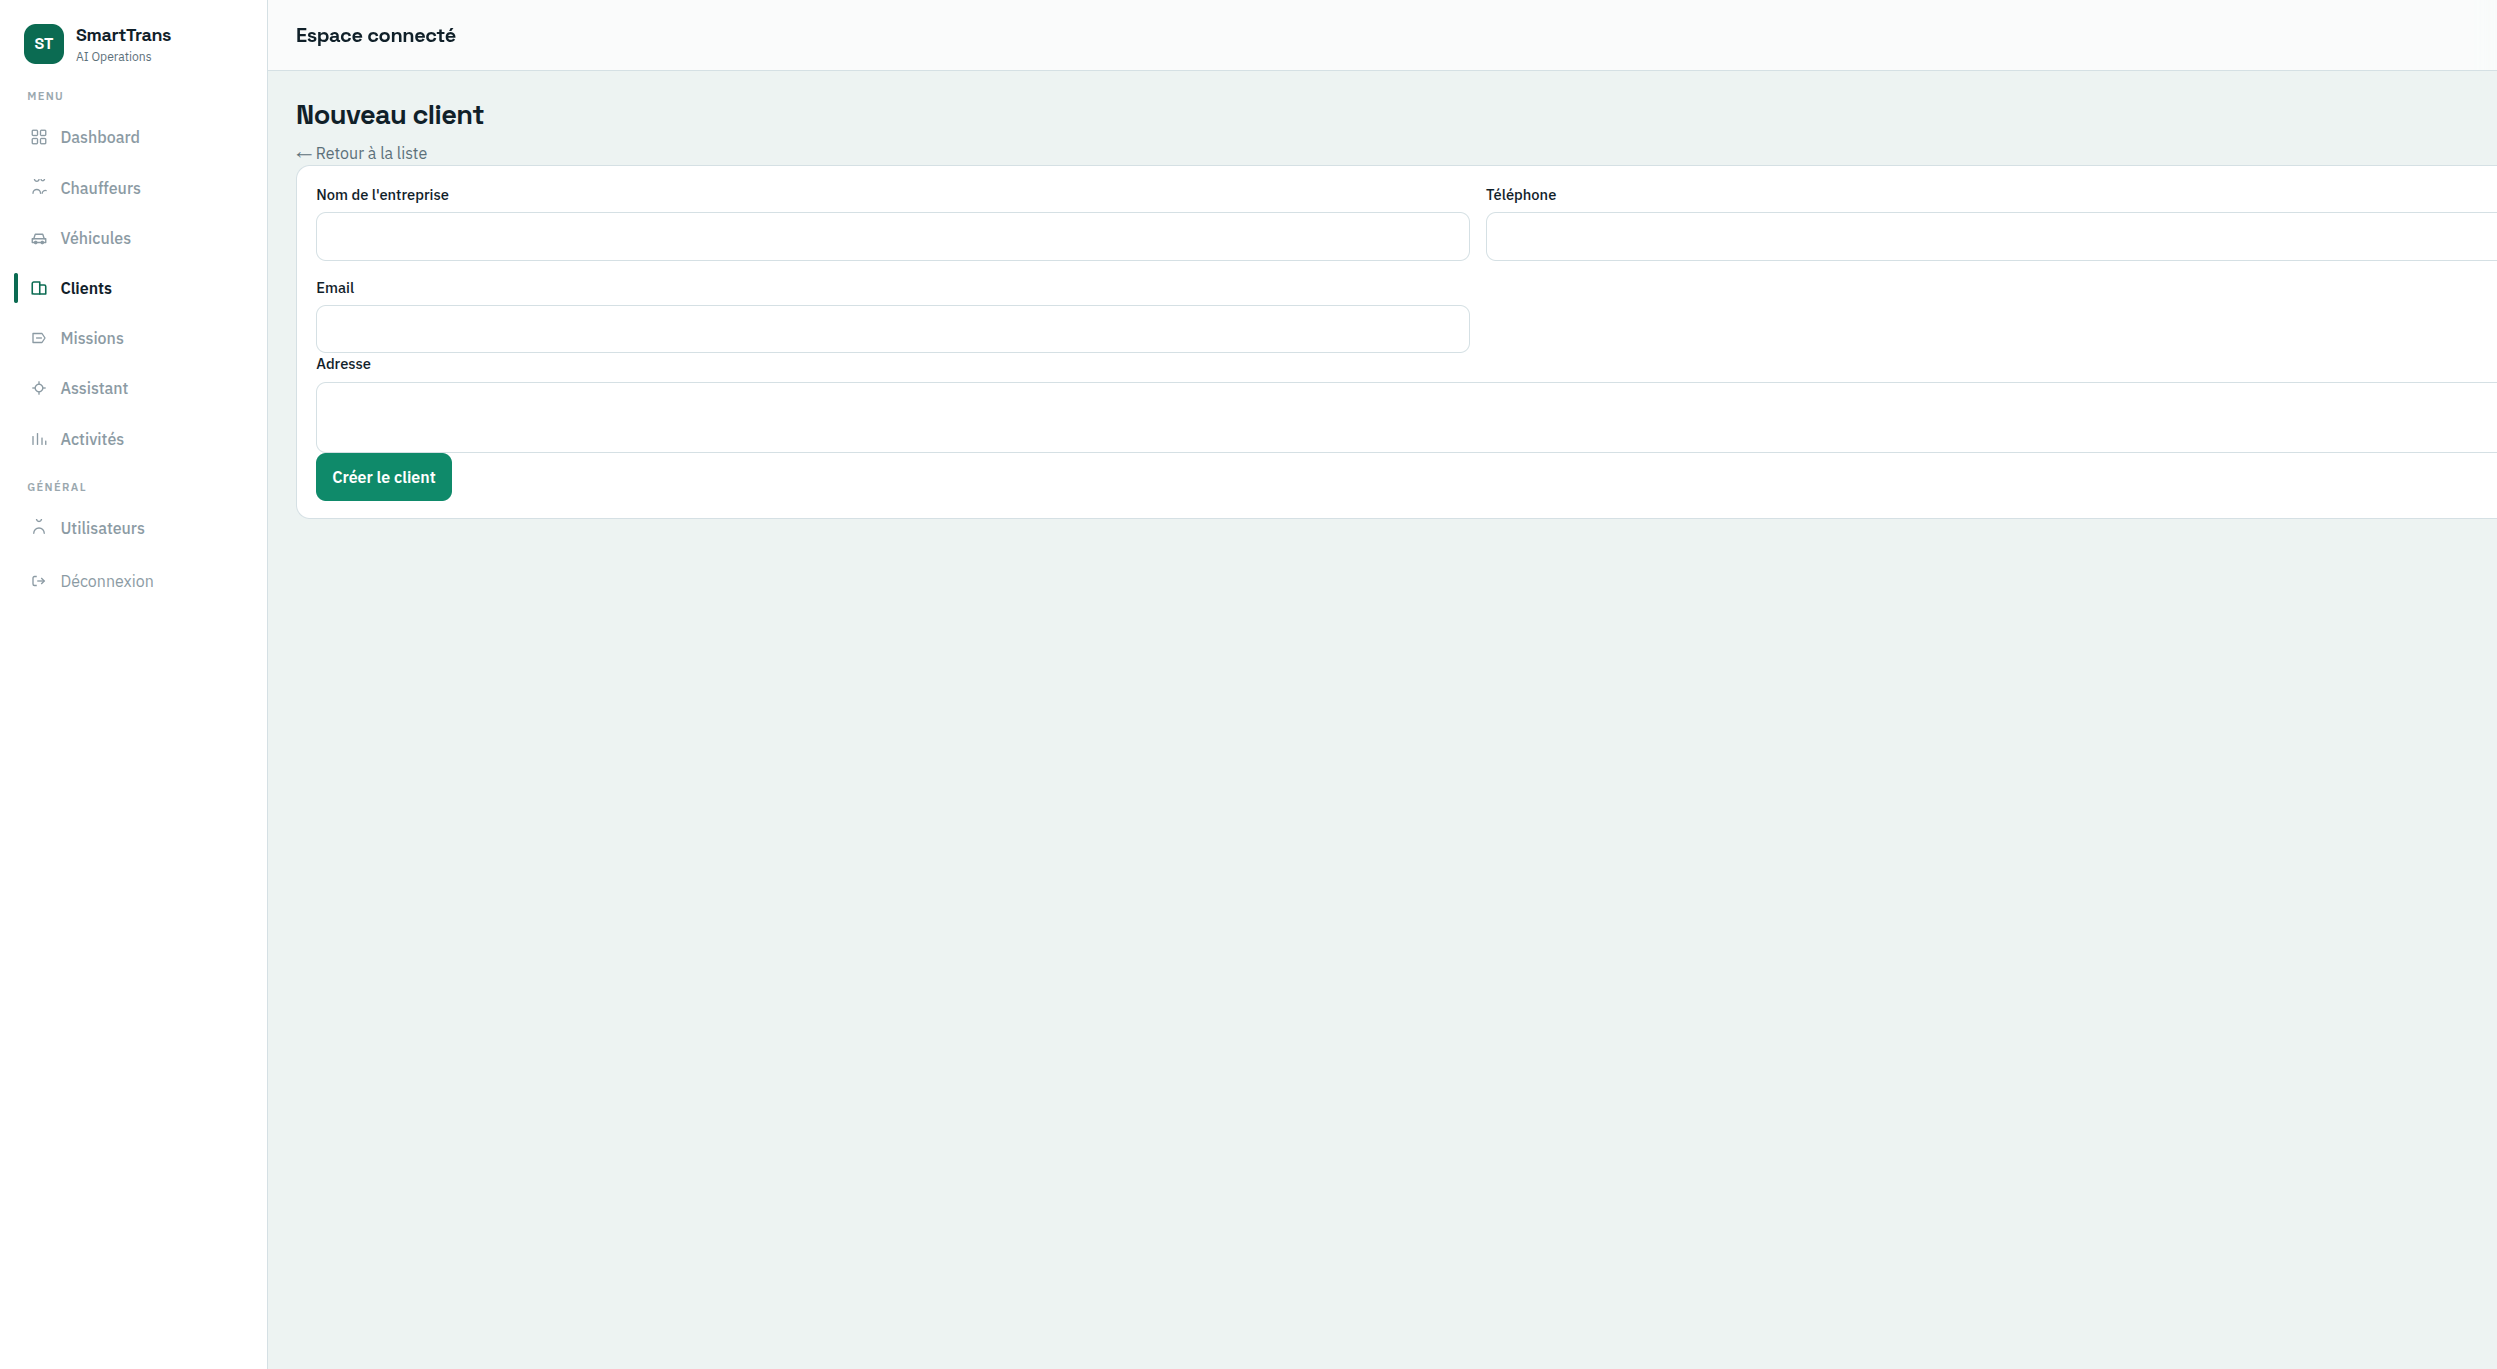
\includegraphics[width=0.88\textwidth,keepaspectratio]{ui-11-client-nouveau.png}
\caption{Formulaire de création d'un client}
\label{fig:ui-cli-new}
\end{figure}

\begin{figure}[htbp]
\centering
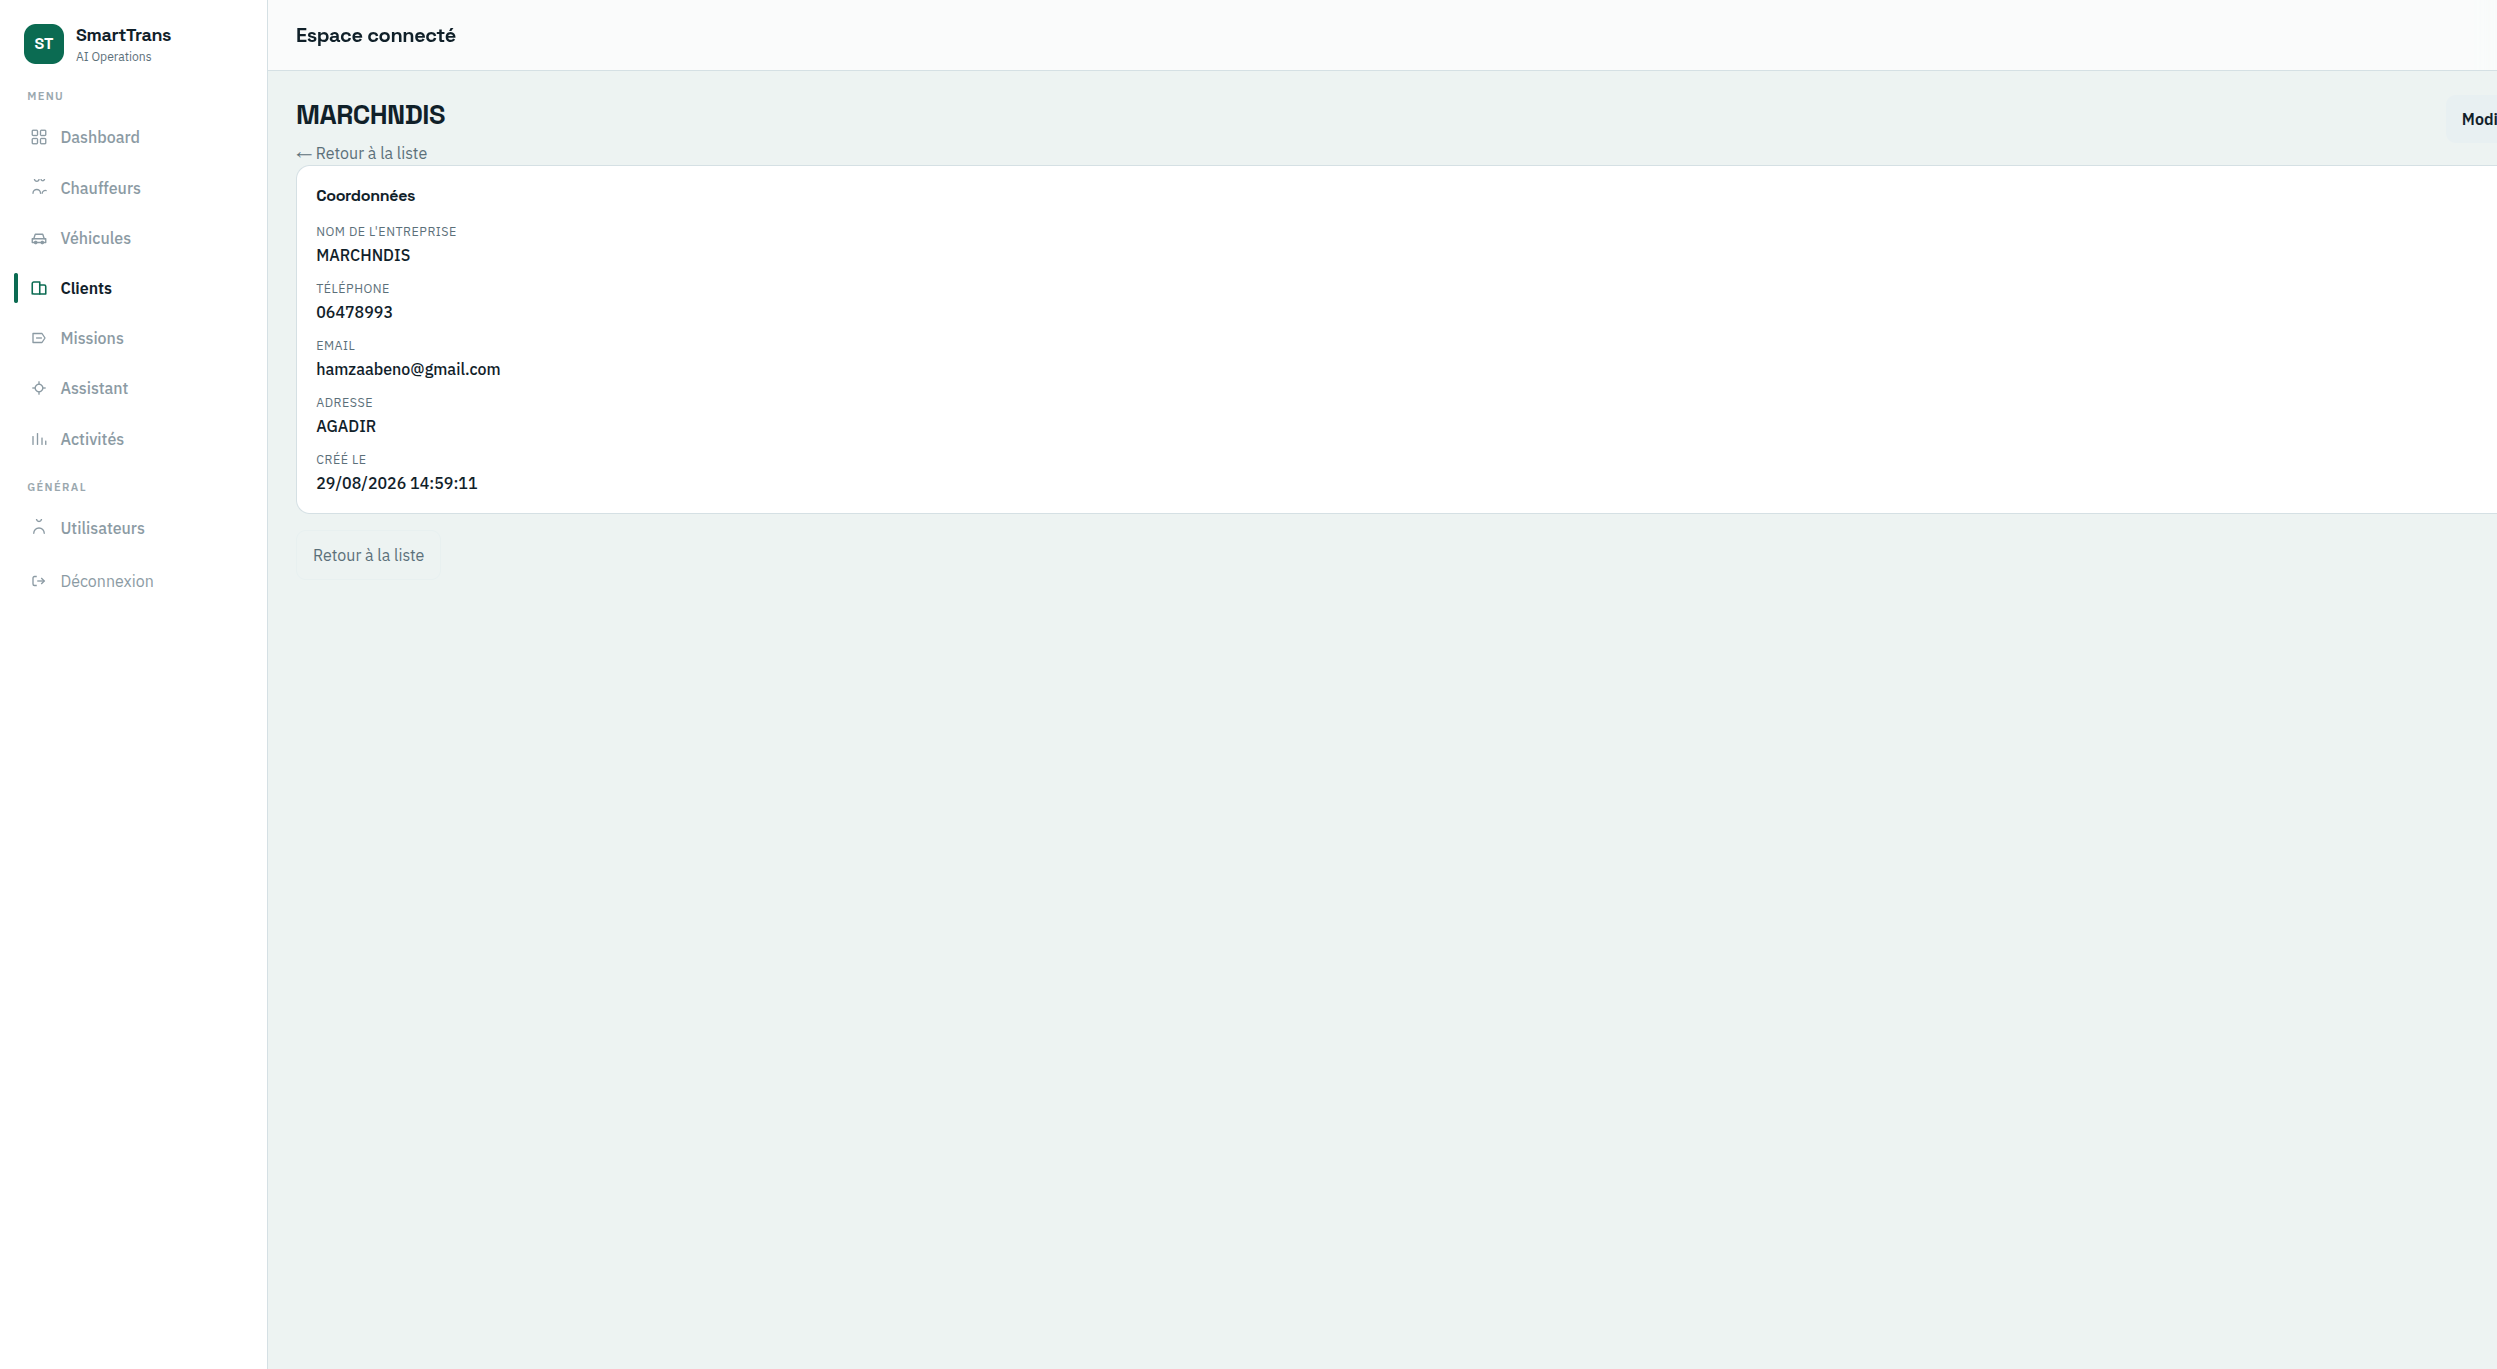
\includegraphics[width=0.88\textwidth,keepaspectratio]{ui-12-client-detail.png}
\caption{Fiche détail d'un client}
\label{fig:ui-cli-det}
\end{figure}

\section{Planification et suivi des missions}

La liste (figure~\ref{fig:ui-mis-list}) relie référence, client, trajet, date, chauffeur, véhicule et statut. Le formulaire de création (figure~\ref{fig:ui-mis-new}) impose une référence, un client et un trajet ; chauffeur et véhicule peuvent rester non assignés. Le détail (figure~\ref{fig:ui-mis-det}) montre l'état d'avancement et les dates de démarrage et de clôture.

\begin{figure}[htbp]
\centering
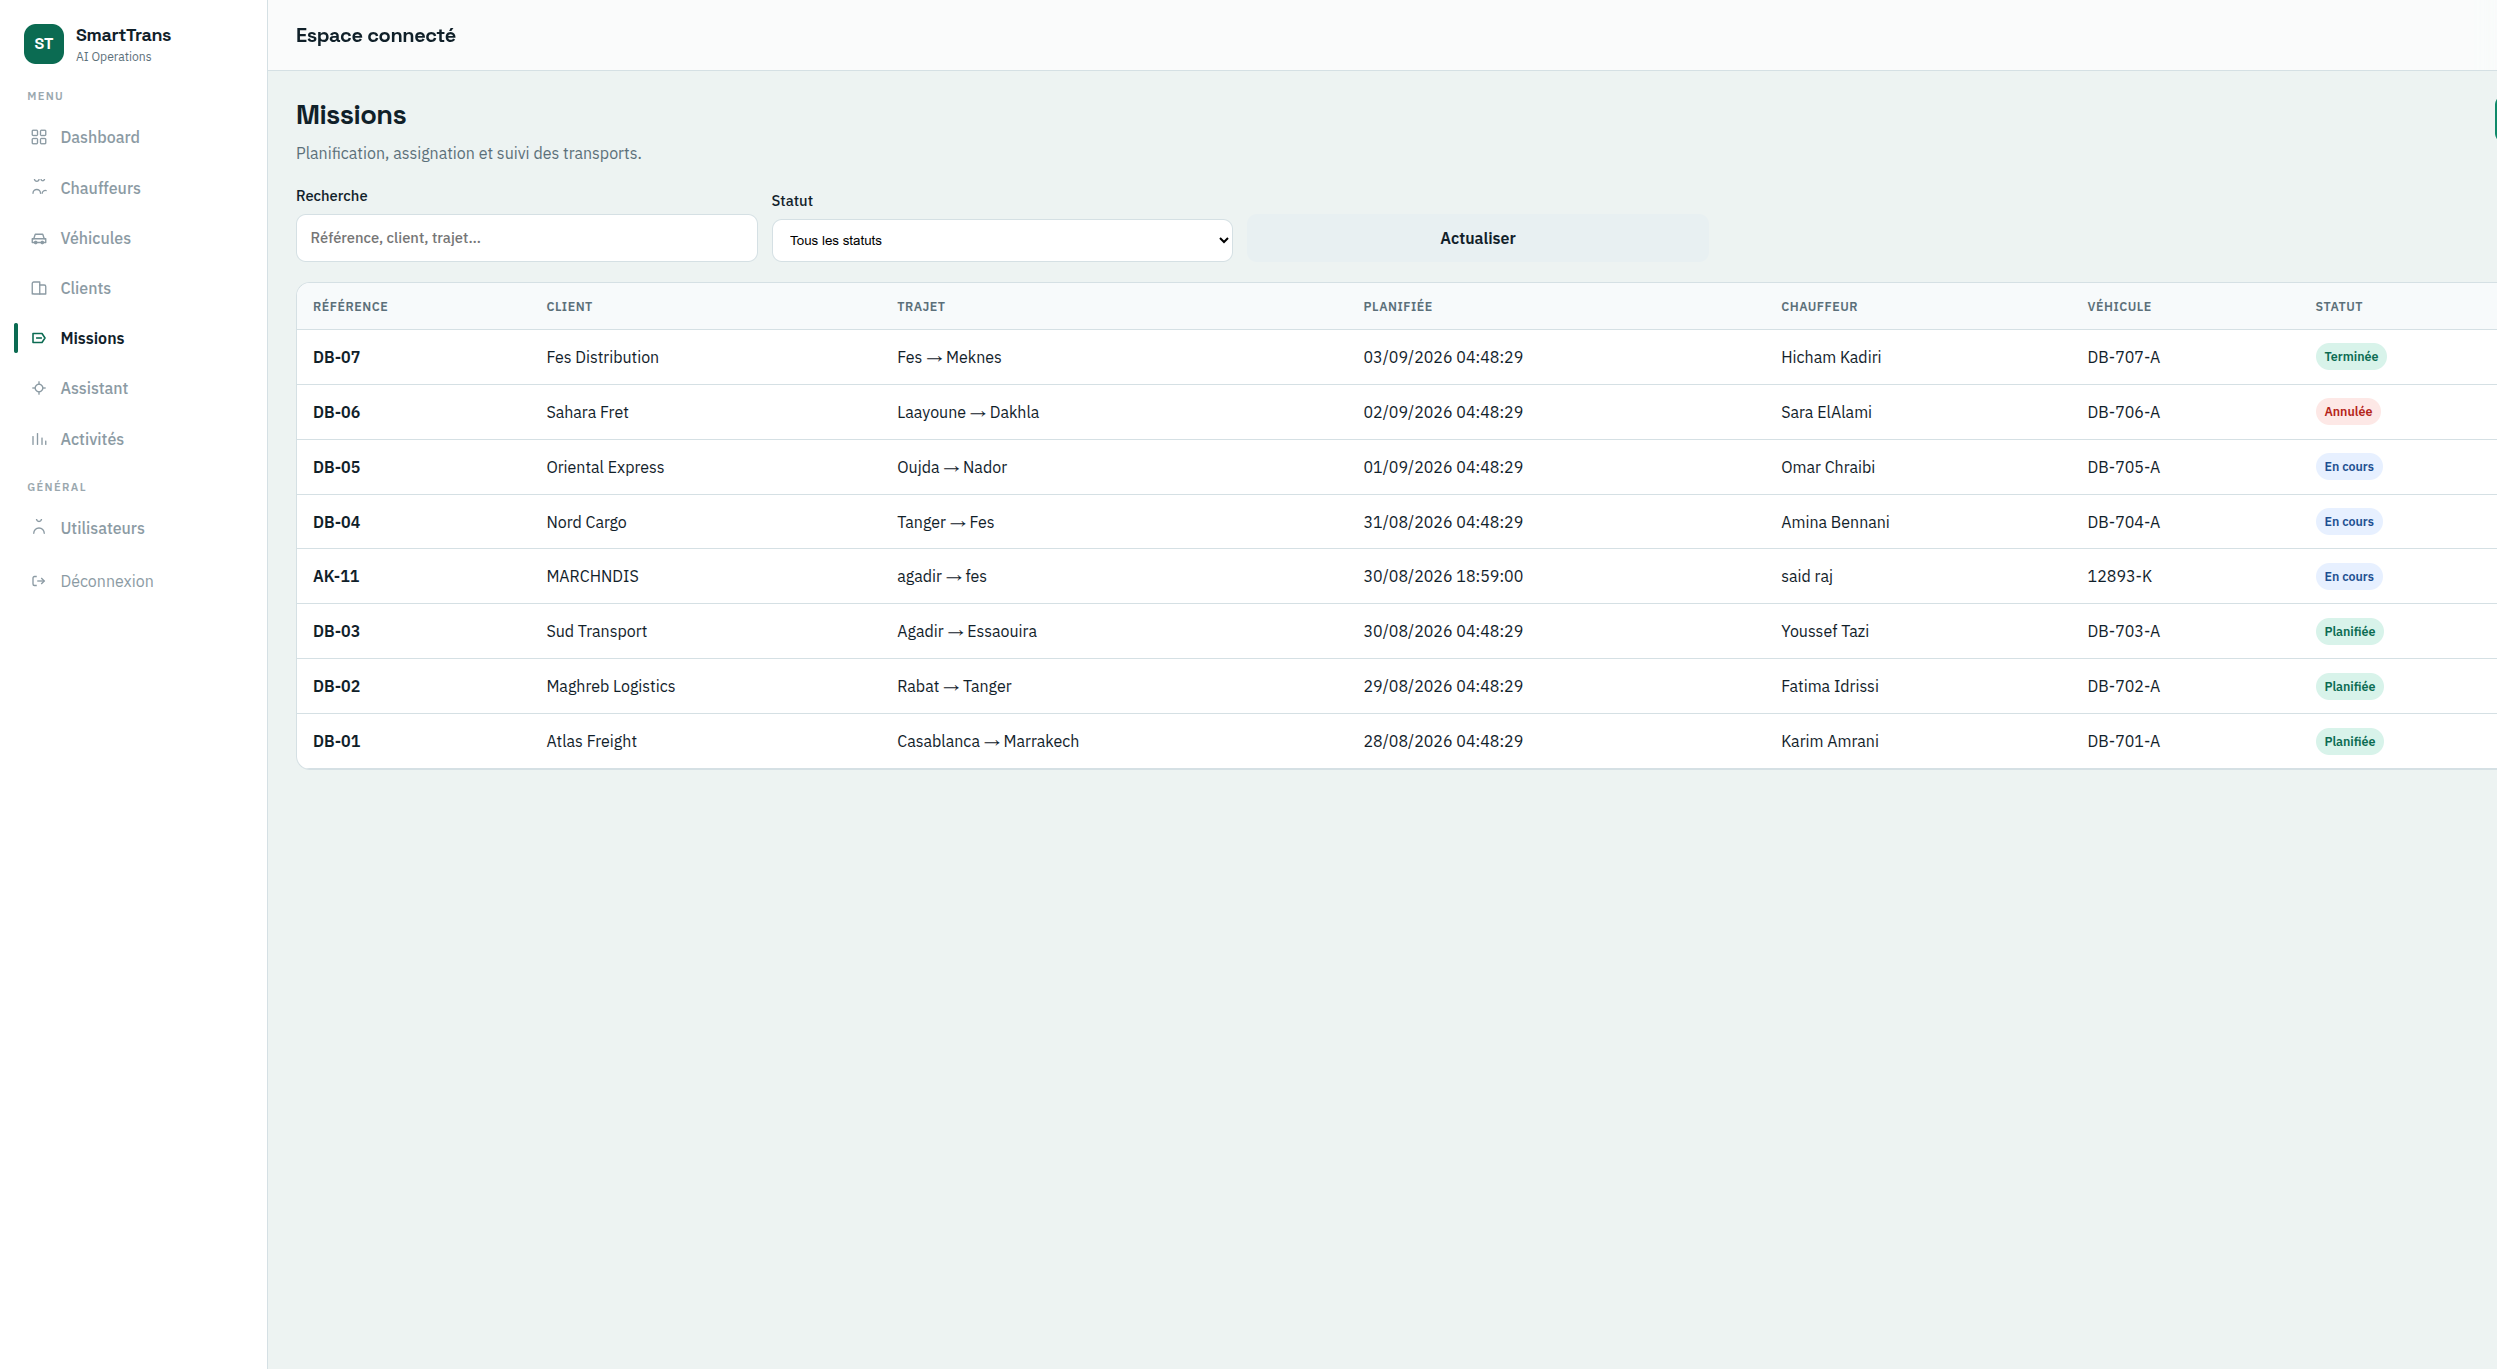
\includegraphics[width=0.95\textwidth,keepaspectratio]{ui-13-missions.png}
\caption{Liste des missions}
\label{fig:ui-mis-list}
\end{figure}

\begin{figure}[htbp]
\centering
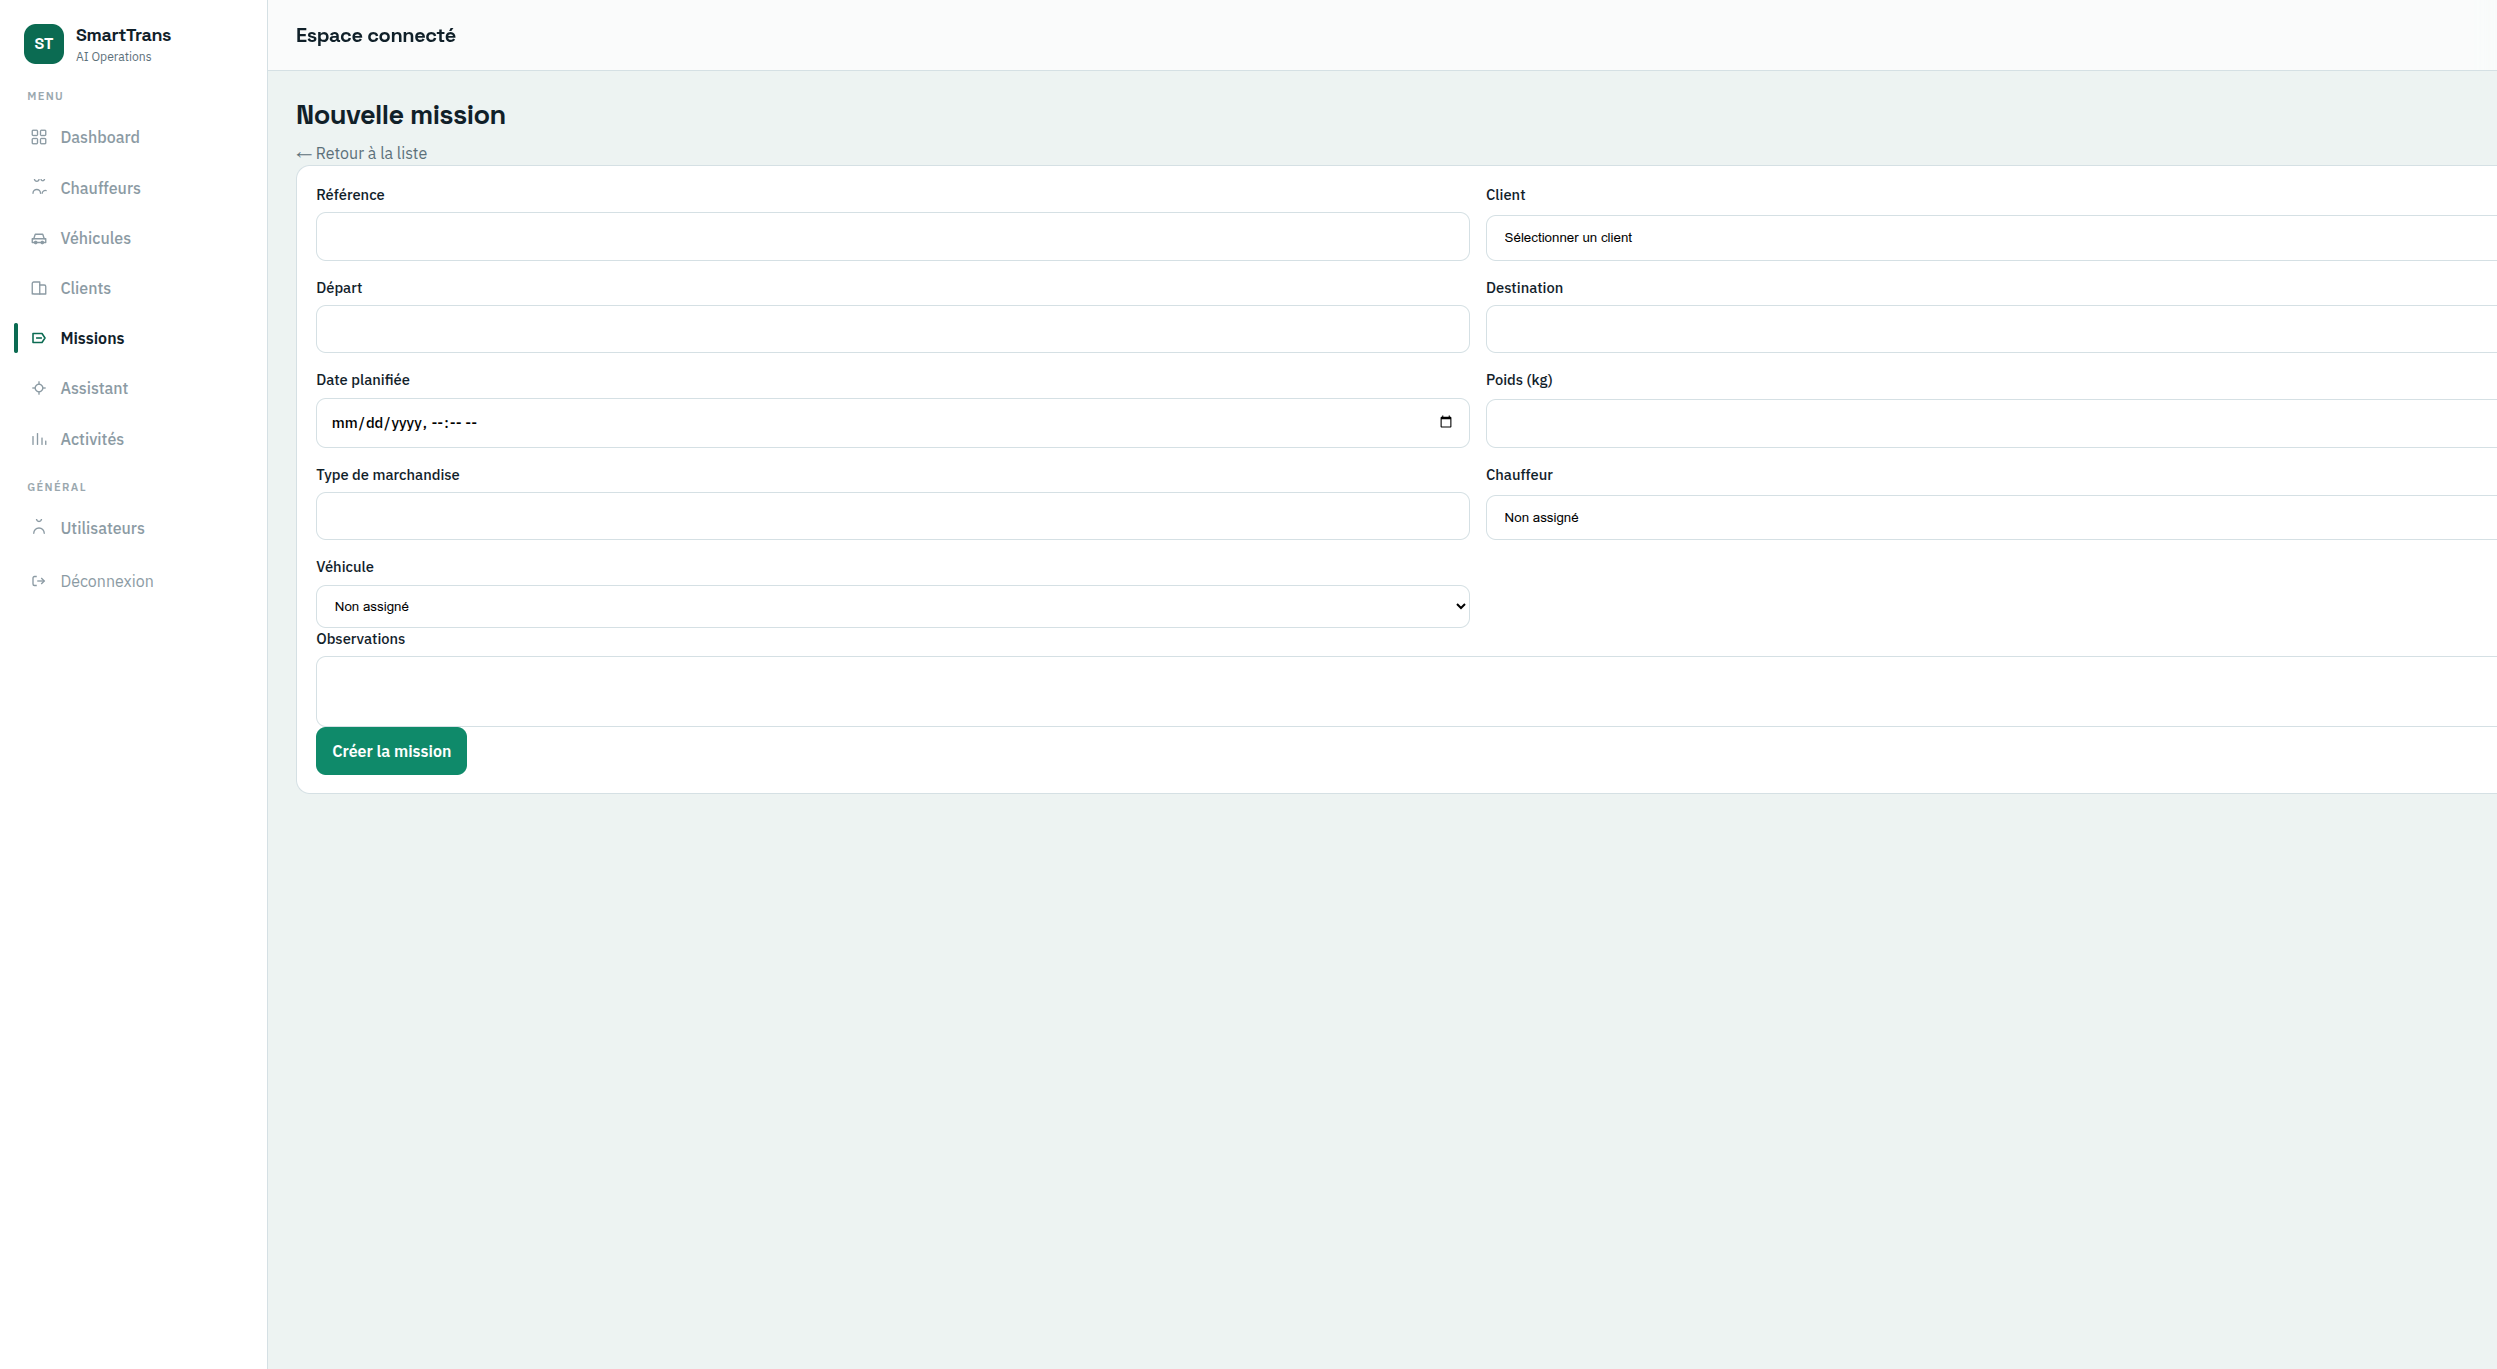
\includegraphics[width=0.88\textwidth,keepaspectratio]{ui-14-mission-nouvelle.png}
\caption{Formulaire de création d'une mission}
\label{fig:ui-mis-new}
\end{figure}

\begin{figure}[htbp]
\centering
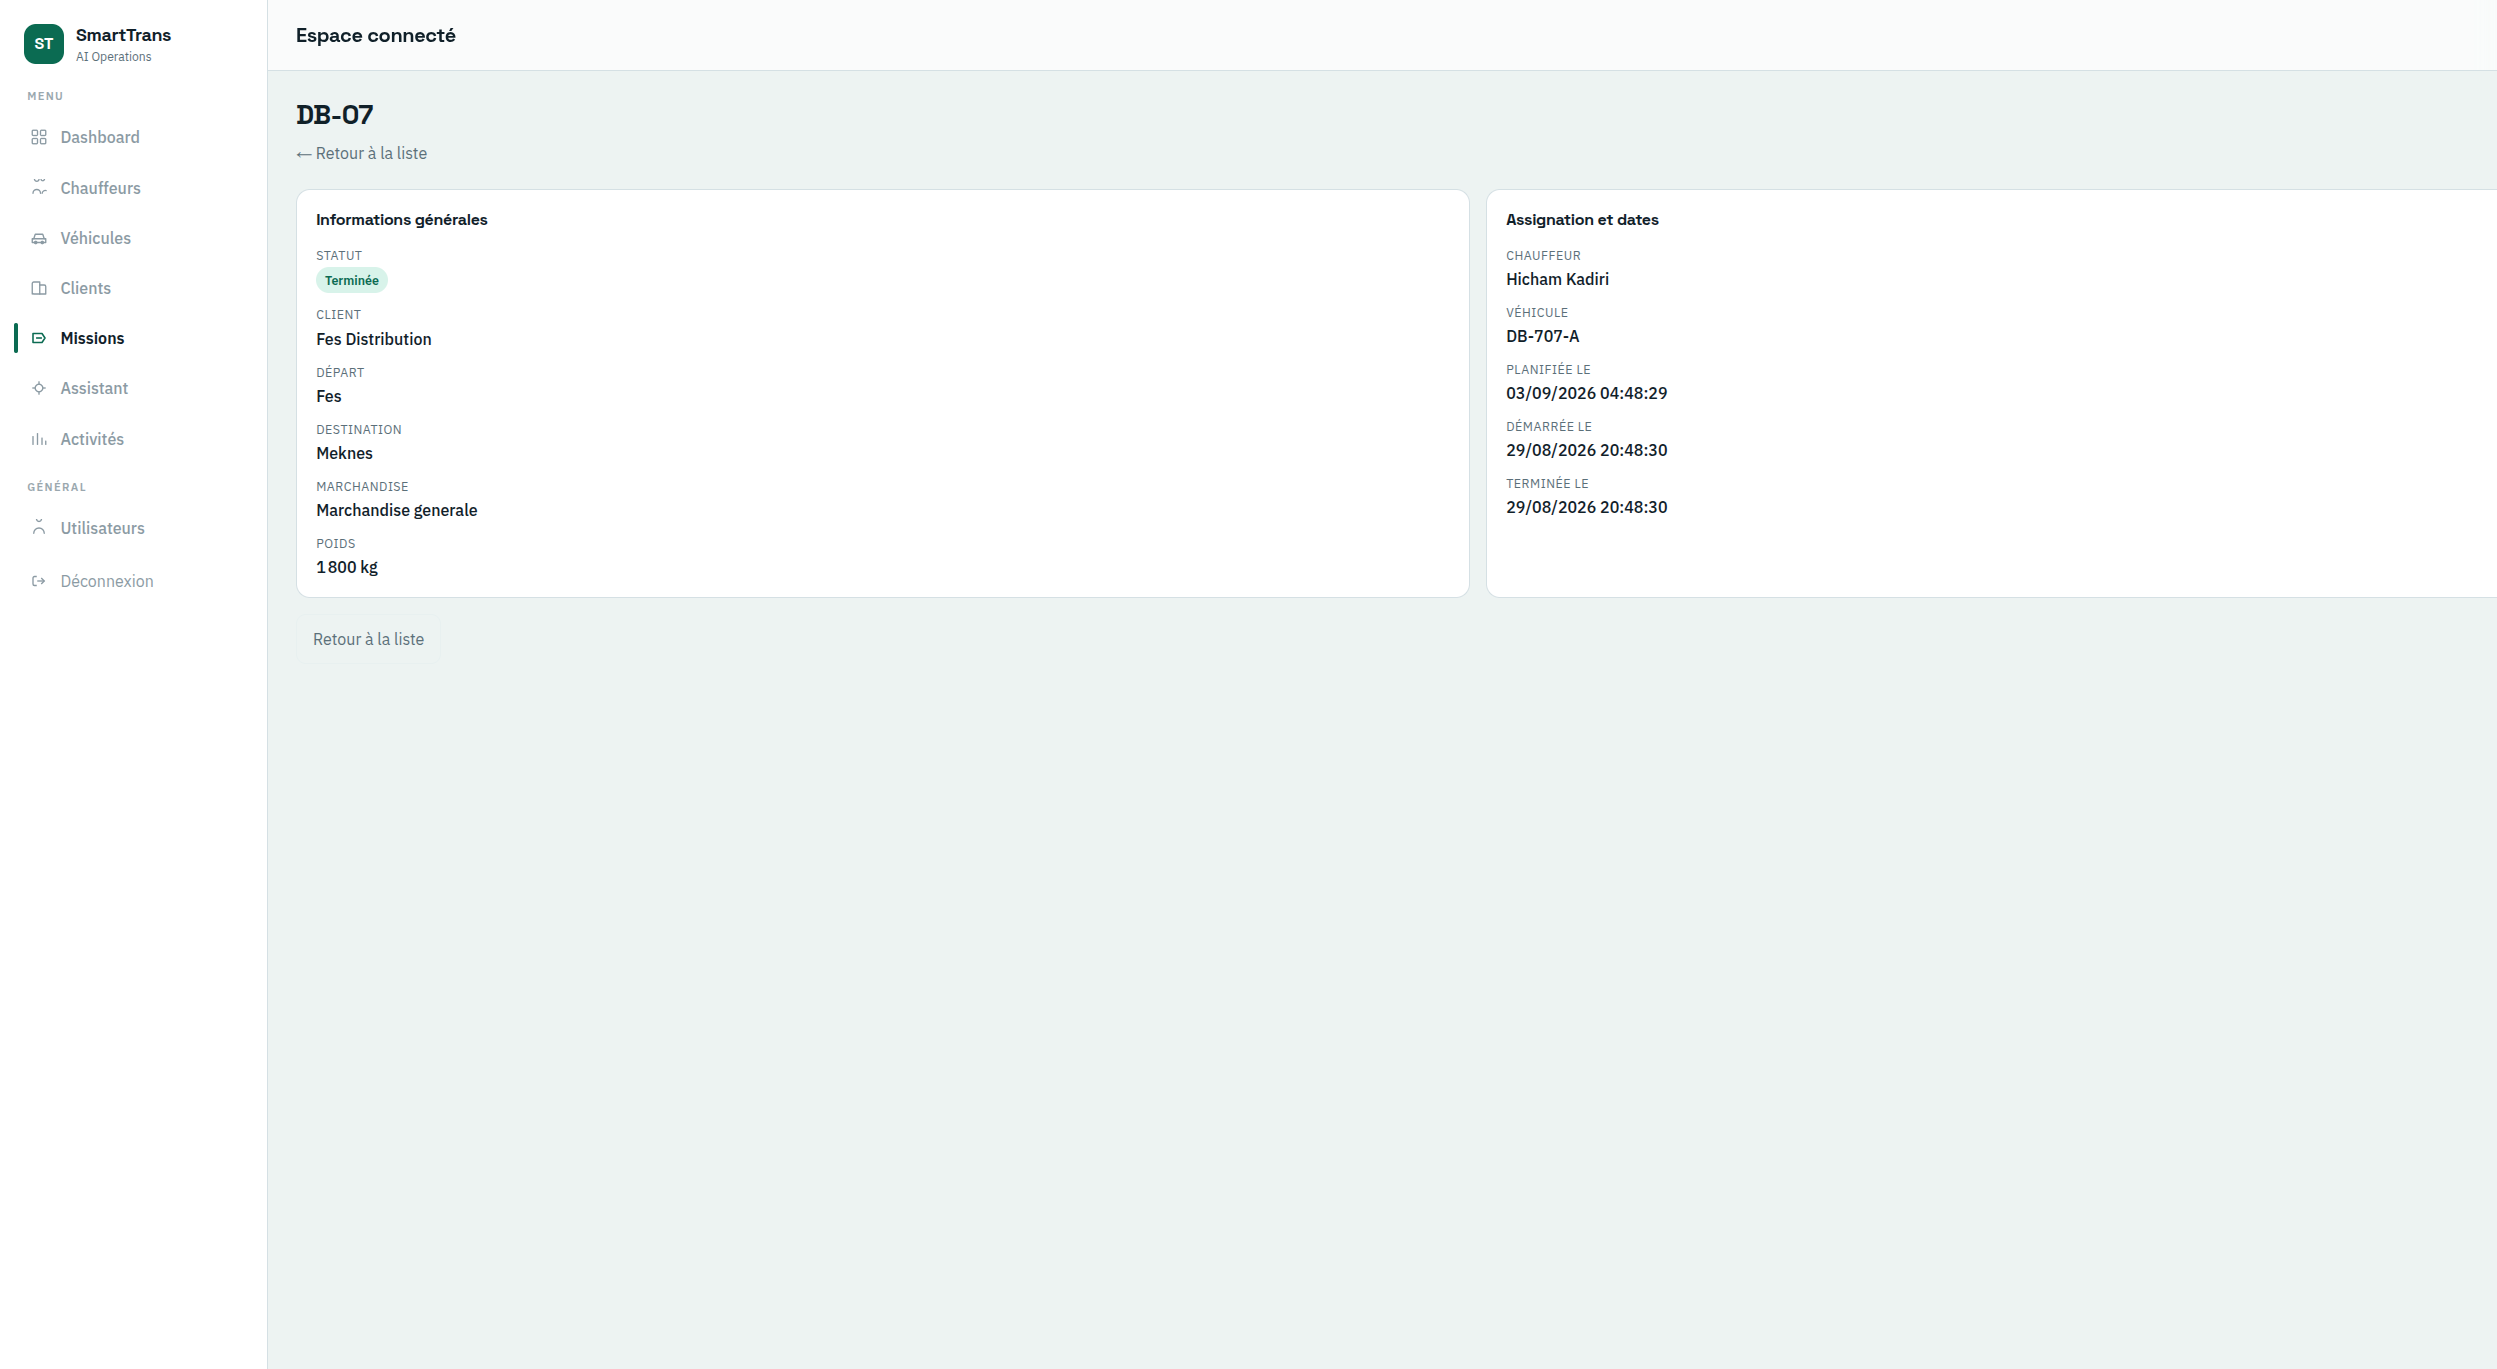
\includegraphics[width=0.88\textwidth,keepaspectratio]{ui-15-mission-detail.png}
\caption{Fiche détail d'une mission}
\label{fig:ui-mis-det}
\end{figure}

\section{Assistant}

La figure~\ref{fig:ui-ai} montre l'assistant réservé à l'exploitation. L'utilisateur pose une question en langue naturelle ou choisit une suggestion. La réponse s'appuie sur les données de la base (missions, chauffeurs, véhicules, alertes), afin de limiter les inventions.

\begin{figure}[htbp]
\centering
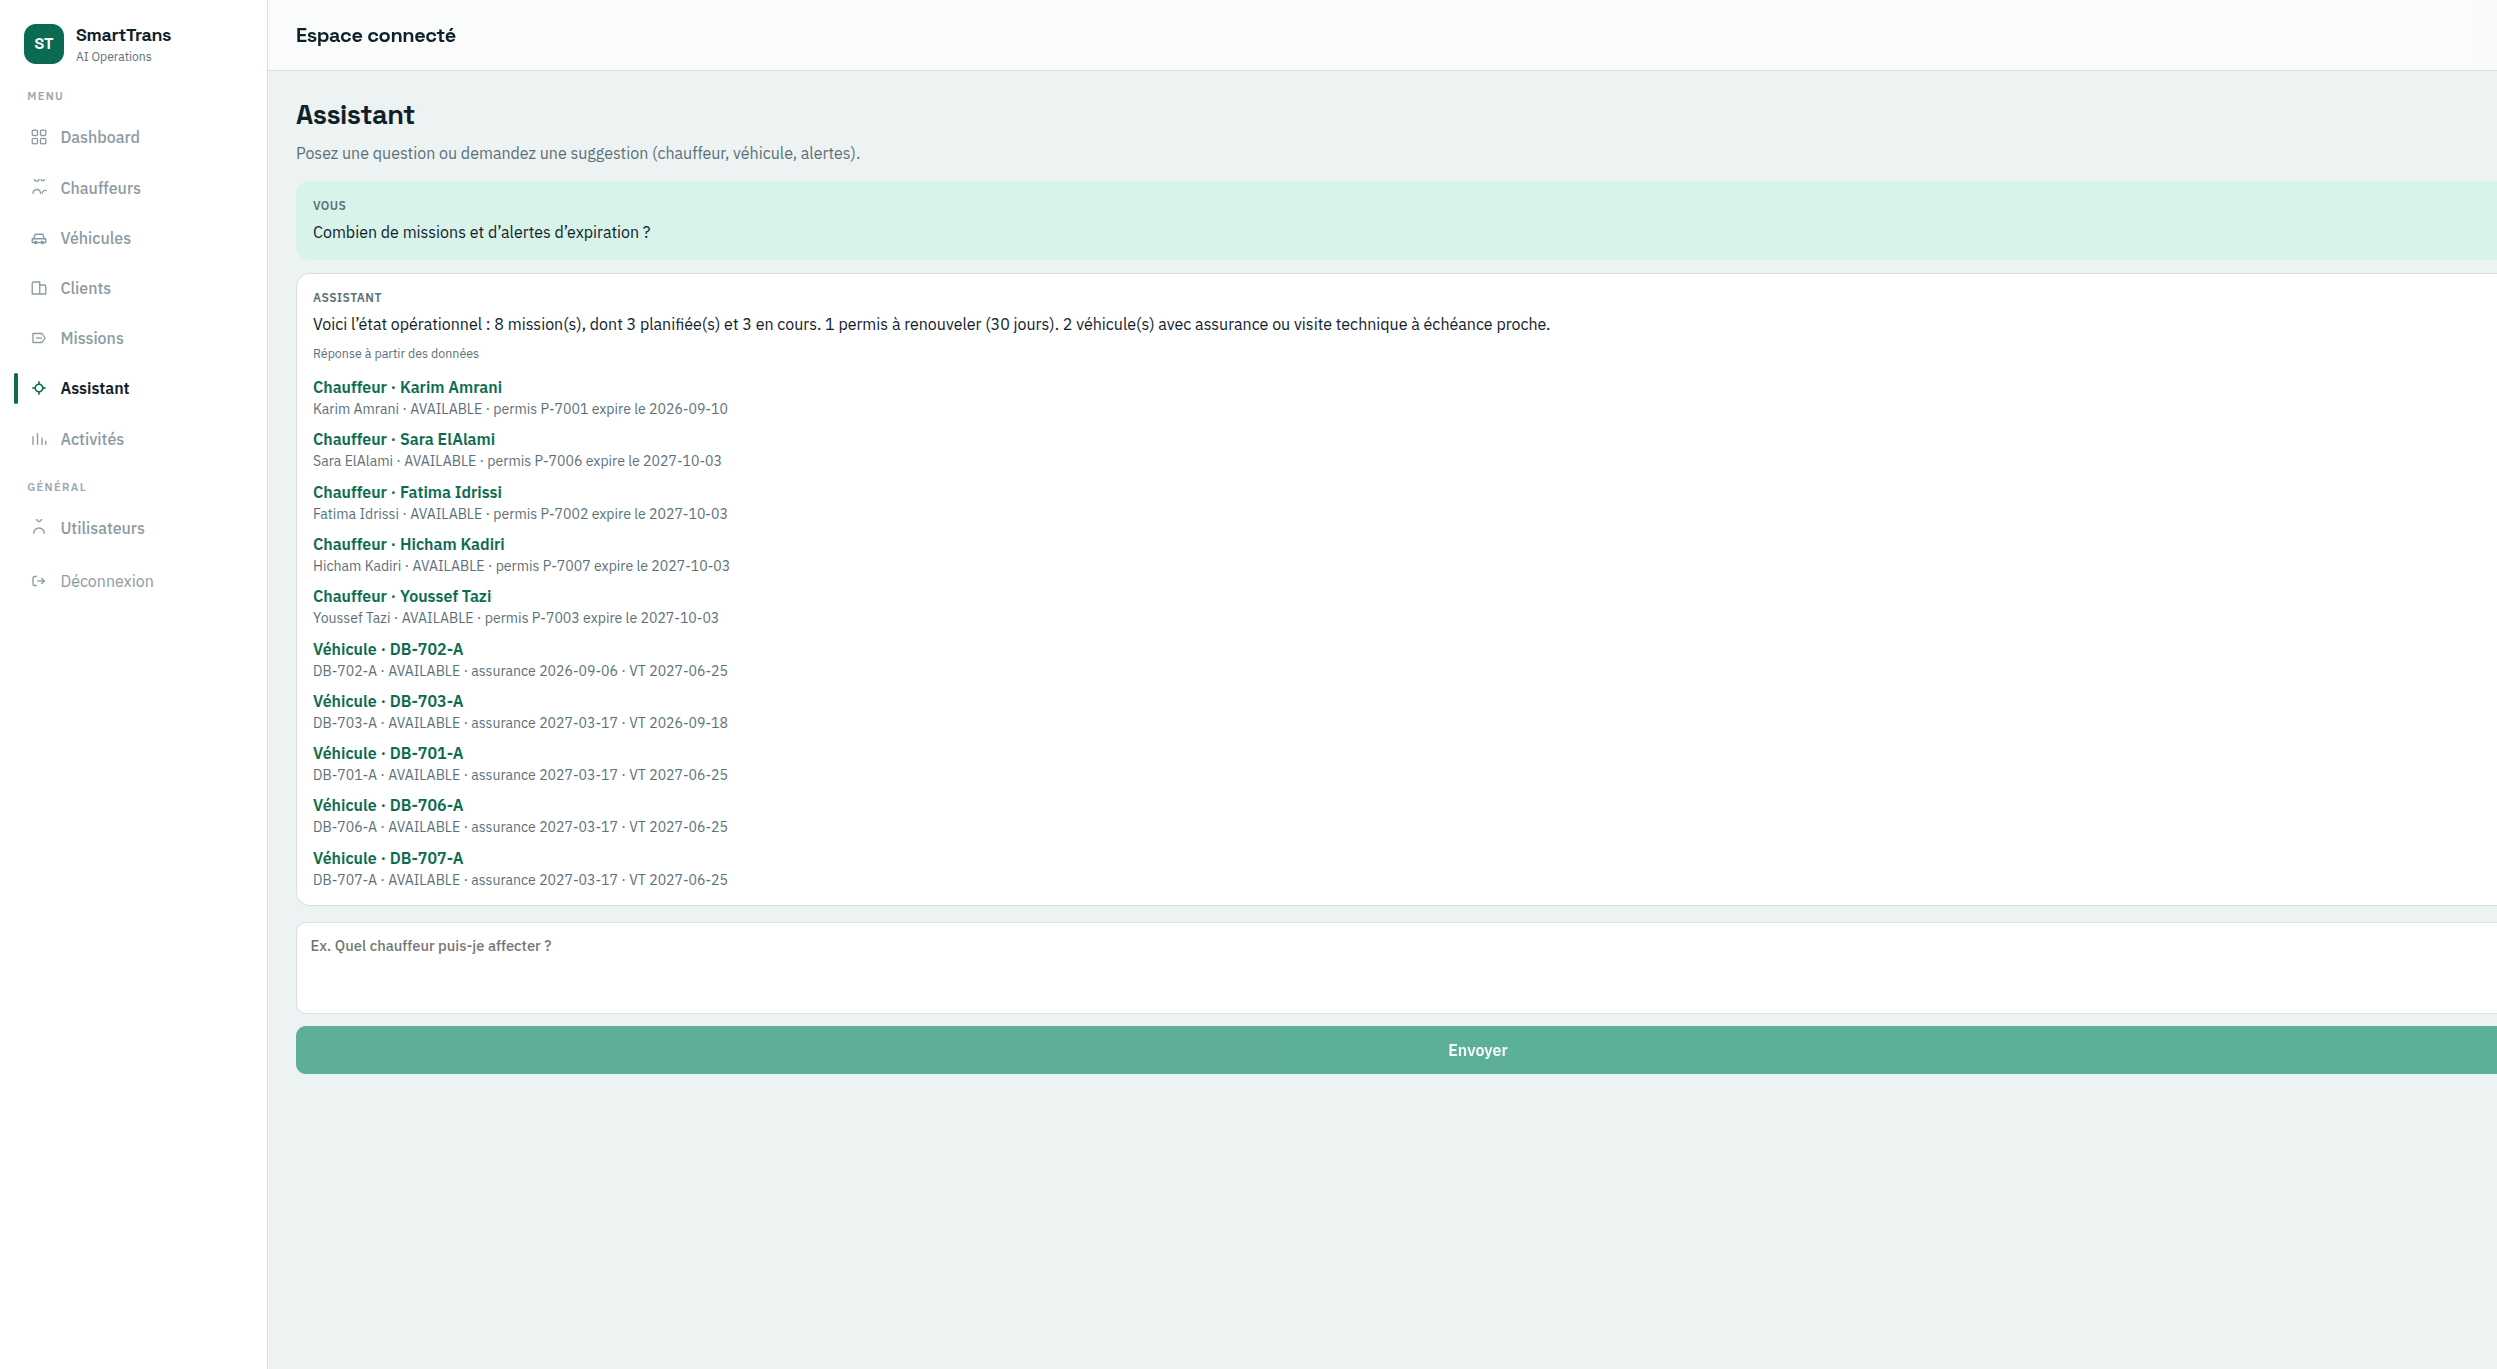
\includegraphics[width=0.95\textwidth,keepaspectratio]{ui-16-assistant.png}
\caption{Assistant conversationnel ancré sur les données métier}
\label{fig:ui-ai}
\end{figure}

\section{Journal d'activités}

La figure~\ref{fig:ui-act} présente le journal en lecture seule. Chaque ligne indique la date, l'action, le type d'entité et un libellé d'objet (courriel, référence de mission, nom, immatriculation). Le filtre par type d'action facilite l'audit.

\begin{figure}[htbp]
\centering
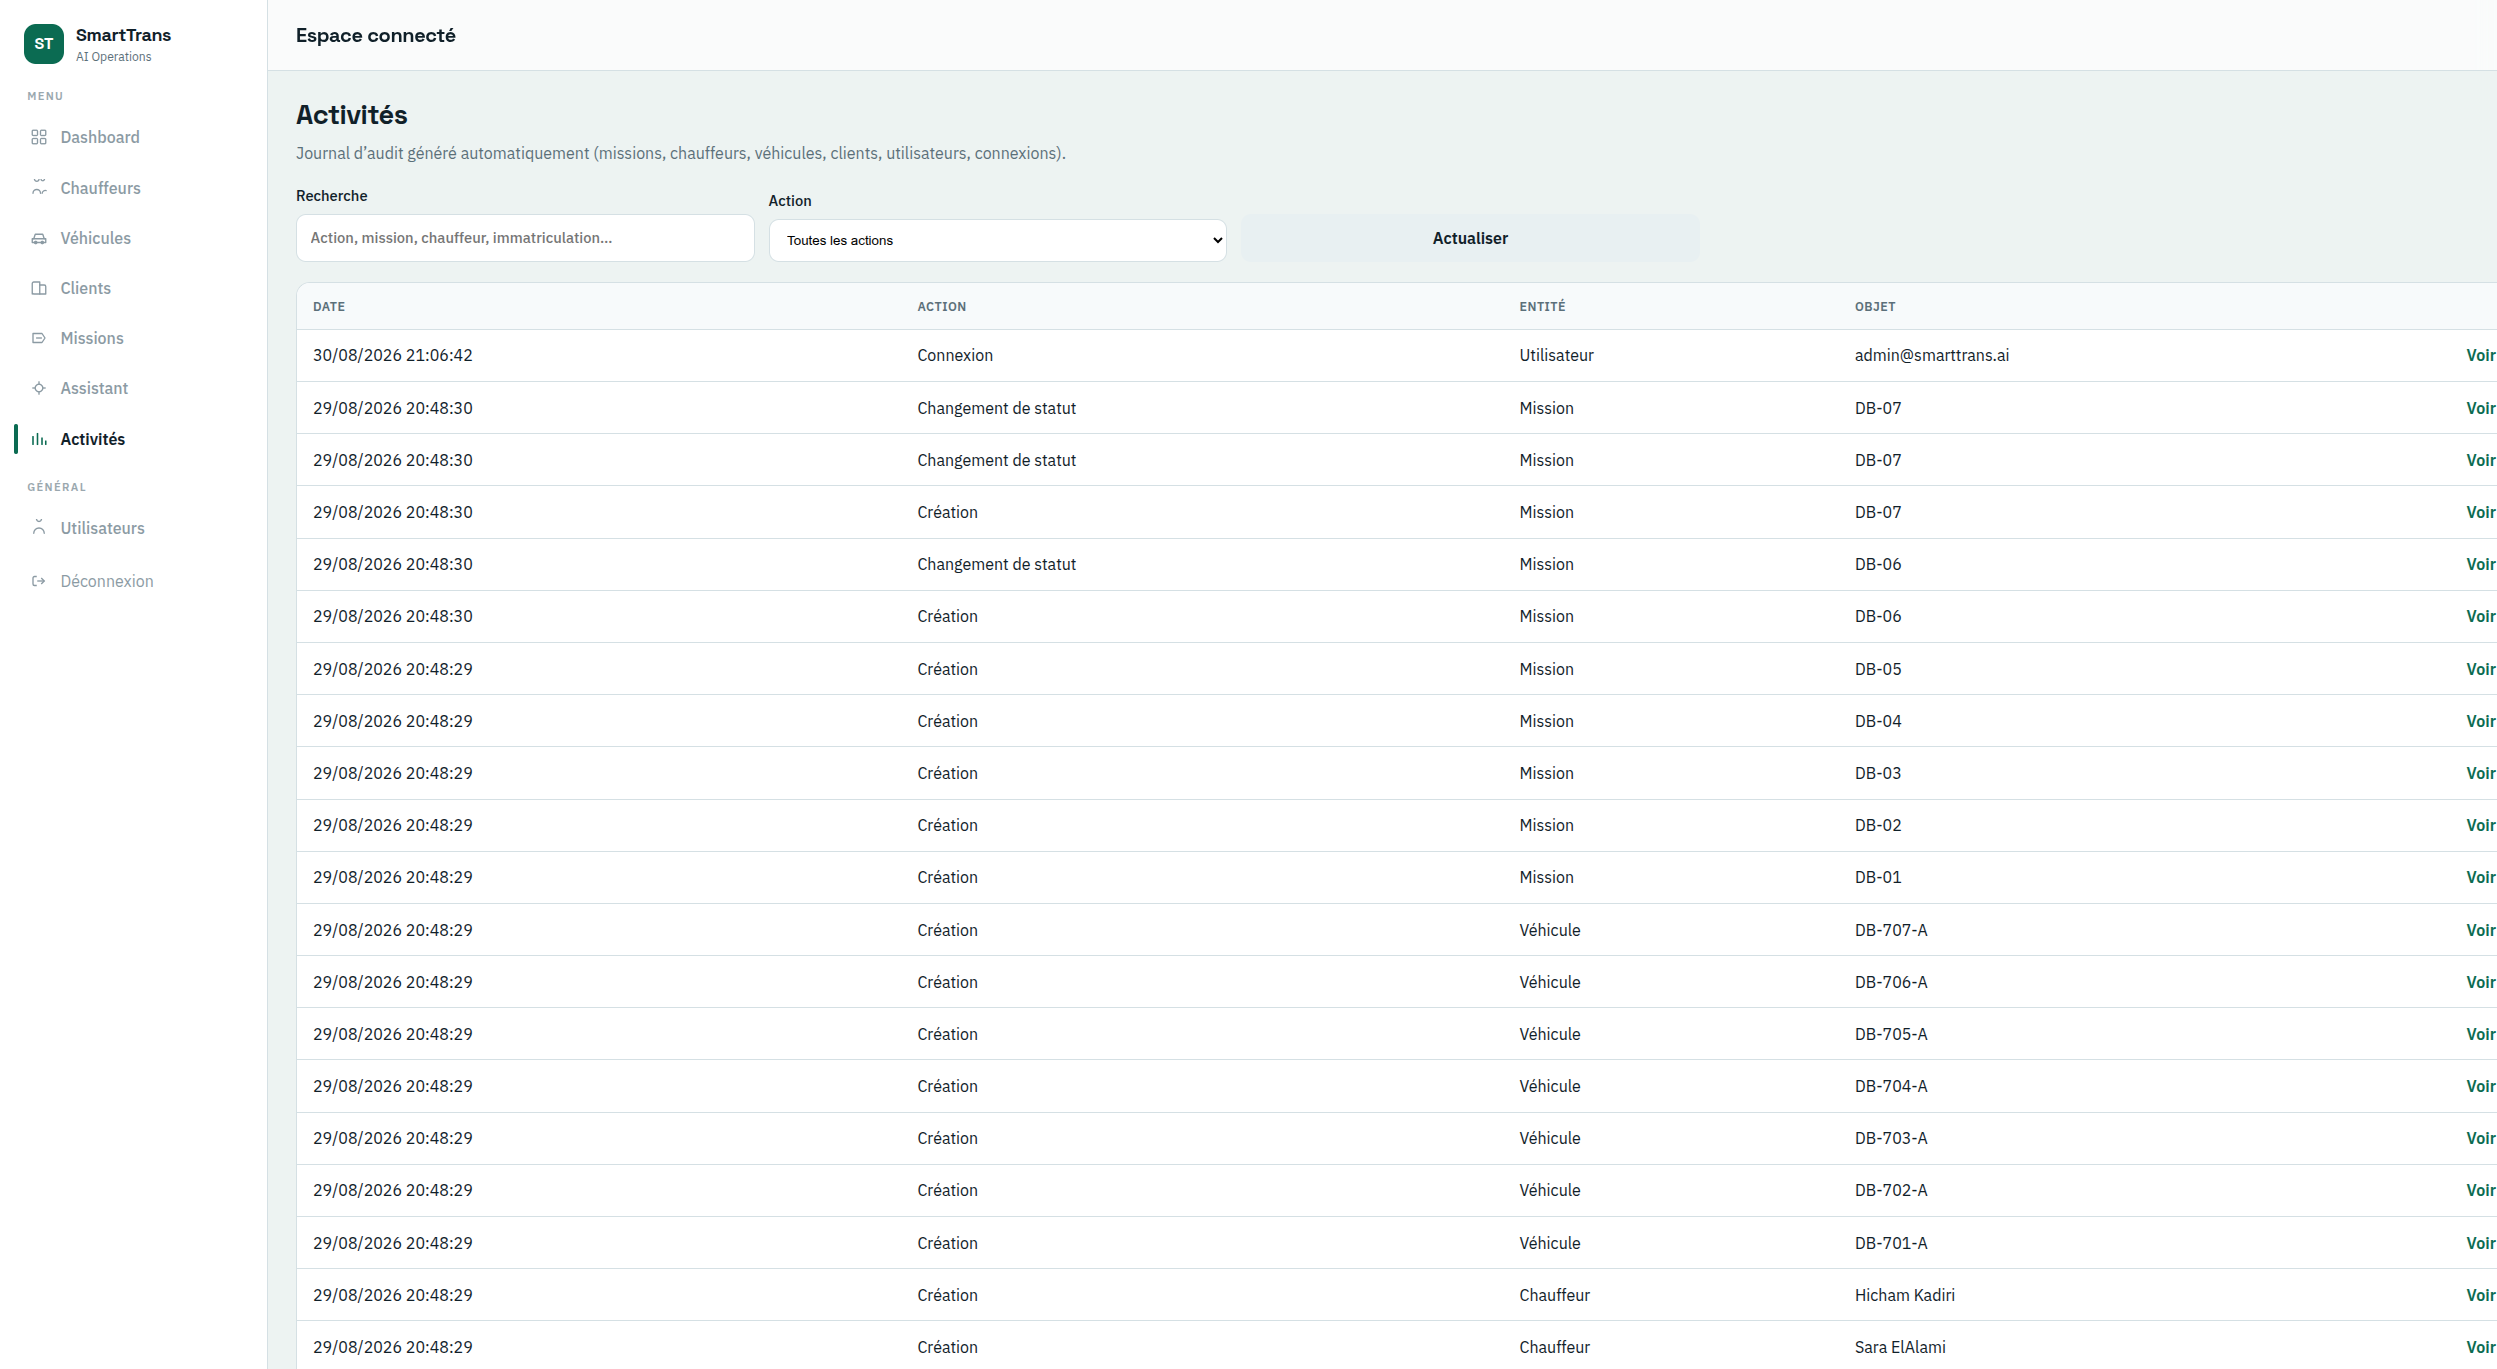
\includegraphics[width=0.95\textwidth,keepaspectratio]{ui-17-activites.png}
\caption{Journal d'activités (audit automatique)}
\label{fig:ui-act}
\end{figure}

\section{Administration : utilisateurs et rôles}

La liste des comptes (figure~\ref{fig:ui-usr}) et le formulaire de création (figure~\ref{fig:ui-usr-new}) sont réservés à l'administrateur. Les rôles (figure~\ref{fig:ui-rol}) correspondent aux trois profils du système : administrateur, responsable transport, chauffeur.

\begin{figure}[htbp]
\centering
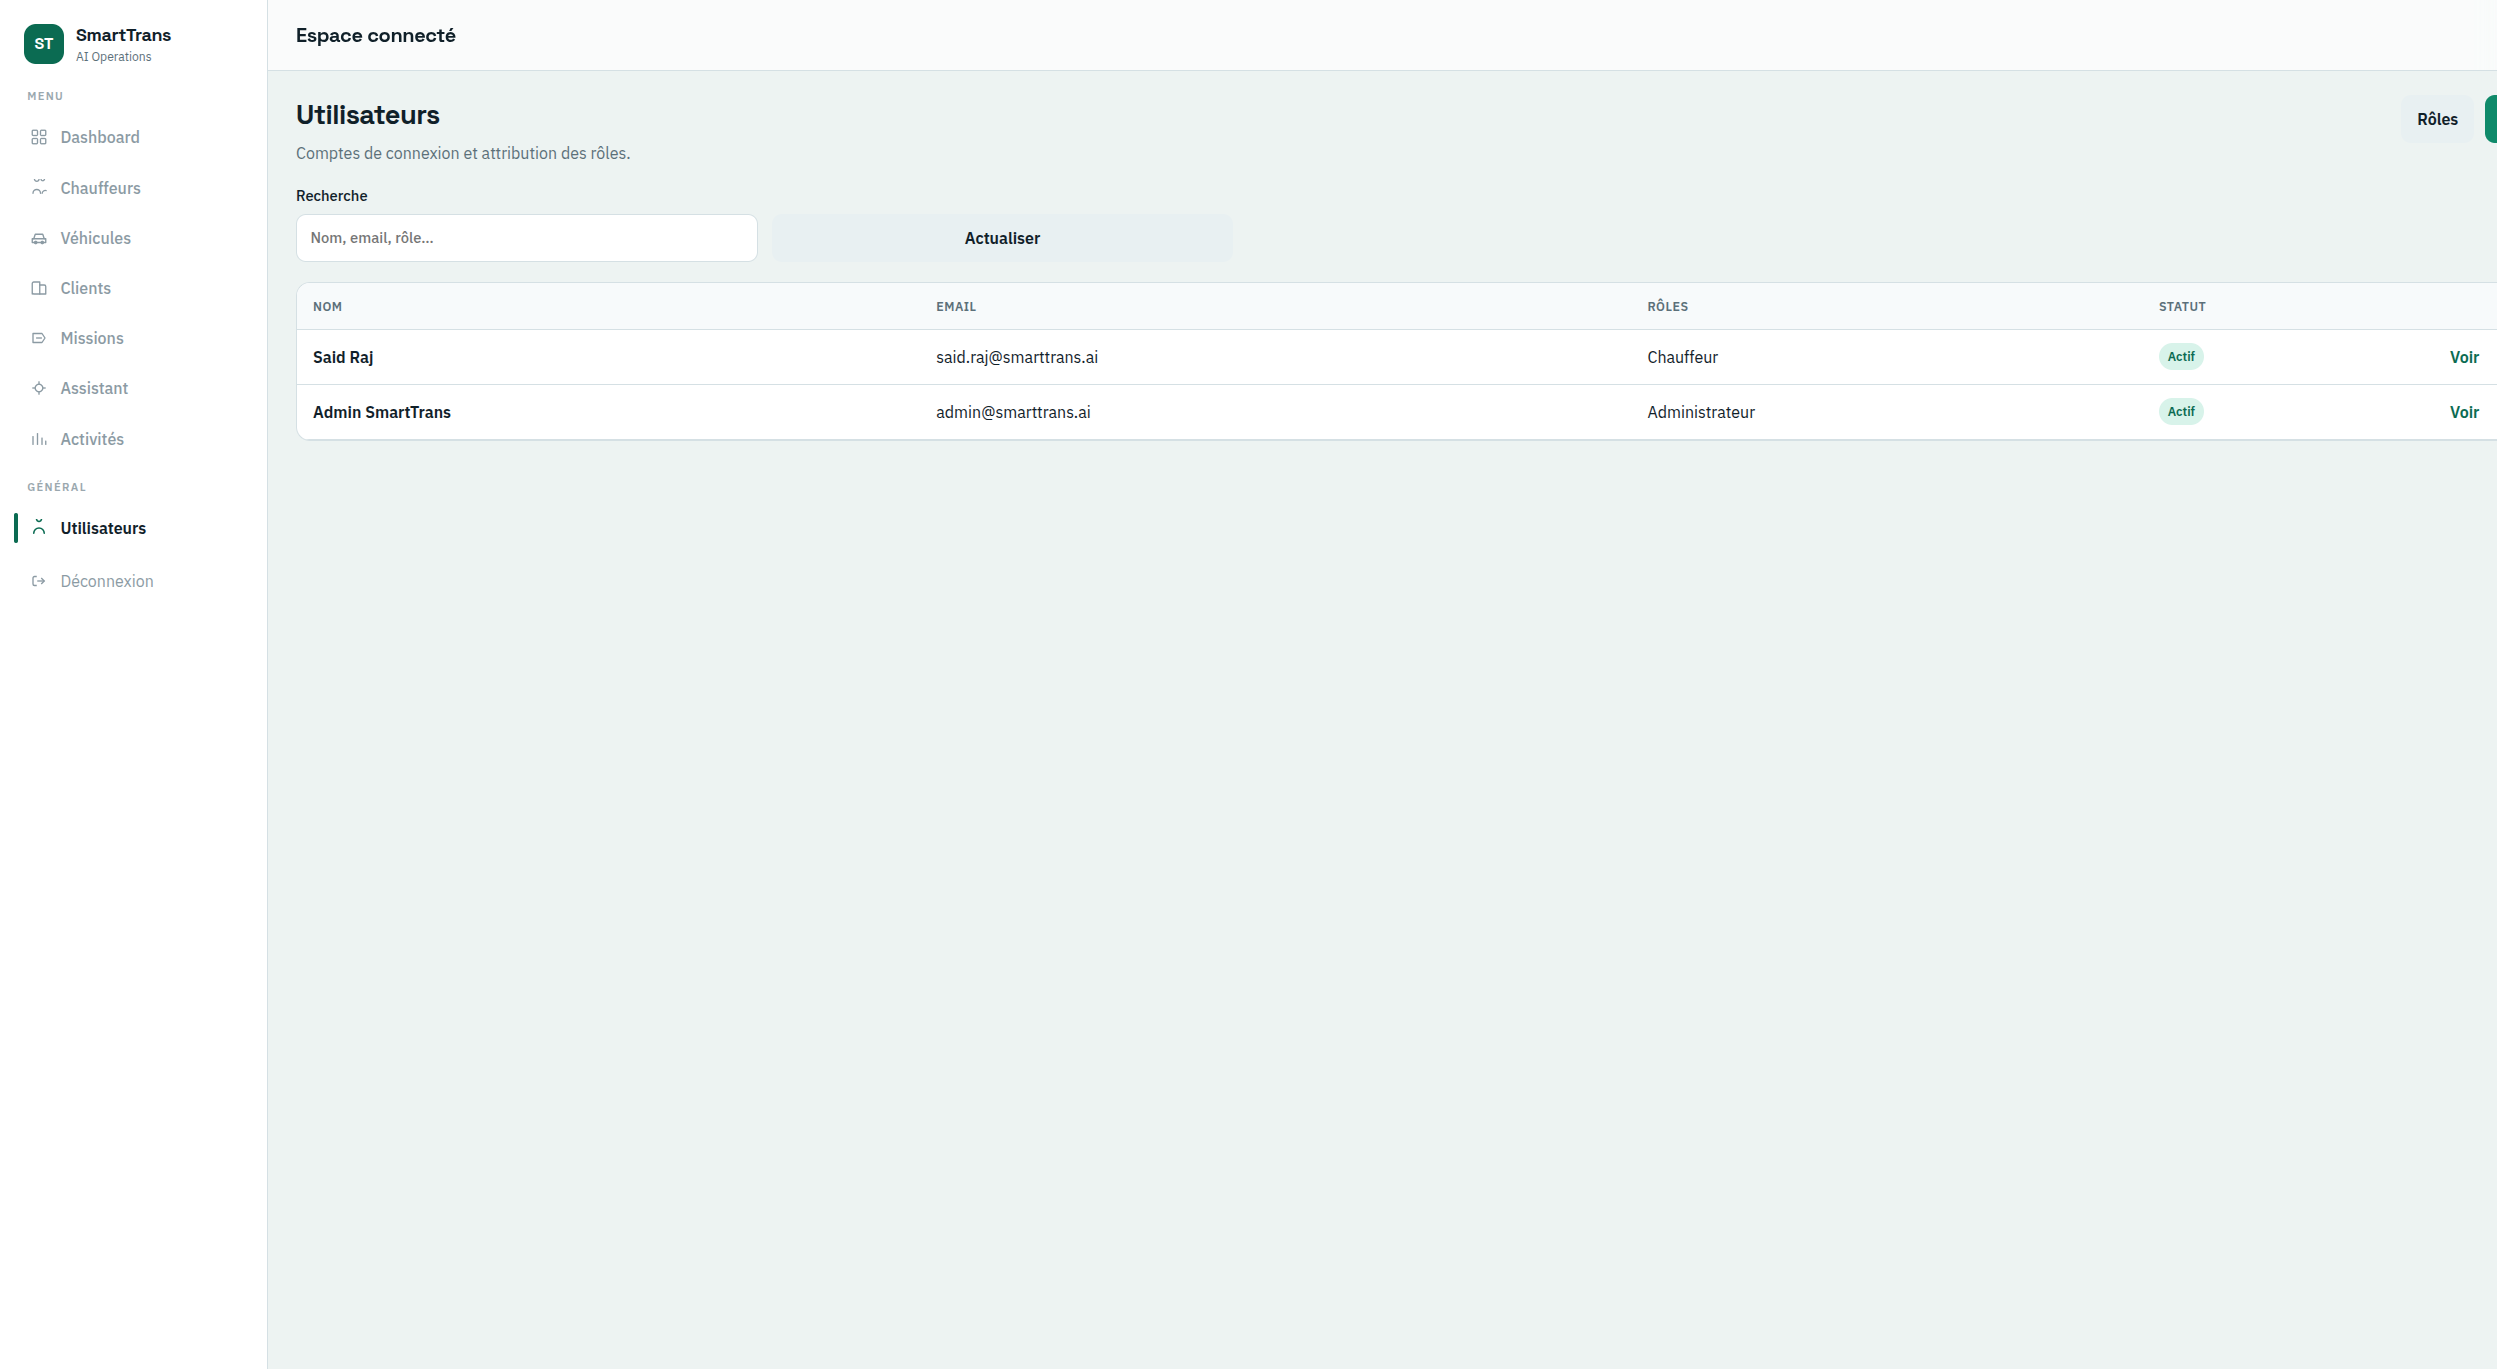
\includegraphics[width=0.95\textwidth,keepaspectratio]{ui-18-utilisateurs.png}
\caption{Liste des utilisateurs}
\label{fig:ui-usr}
\end{figure}

\begin{figure}[htbp]
\centering
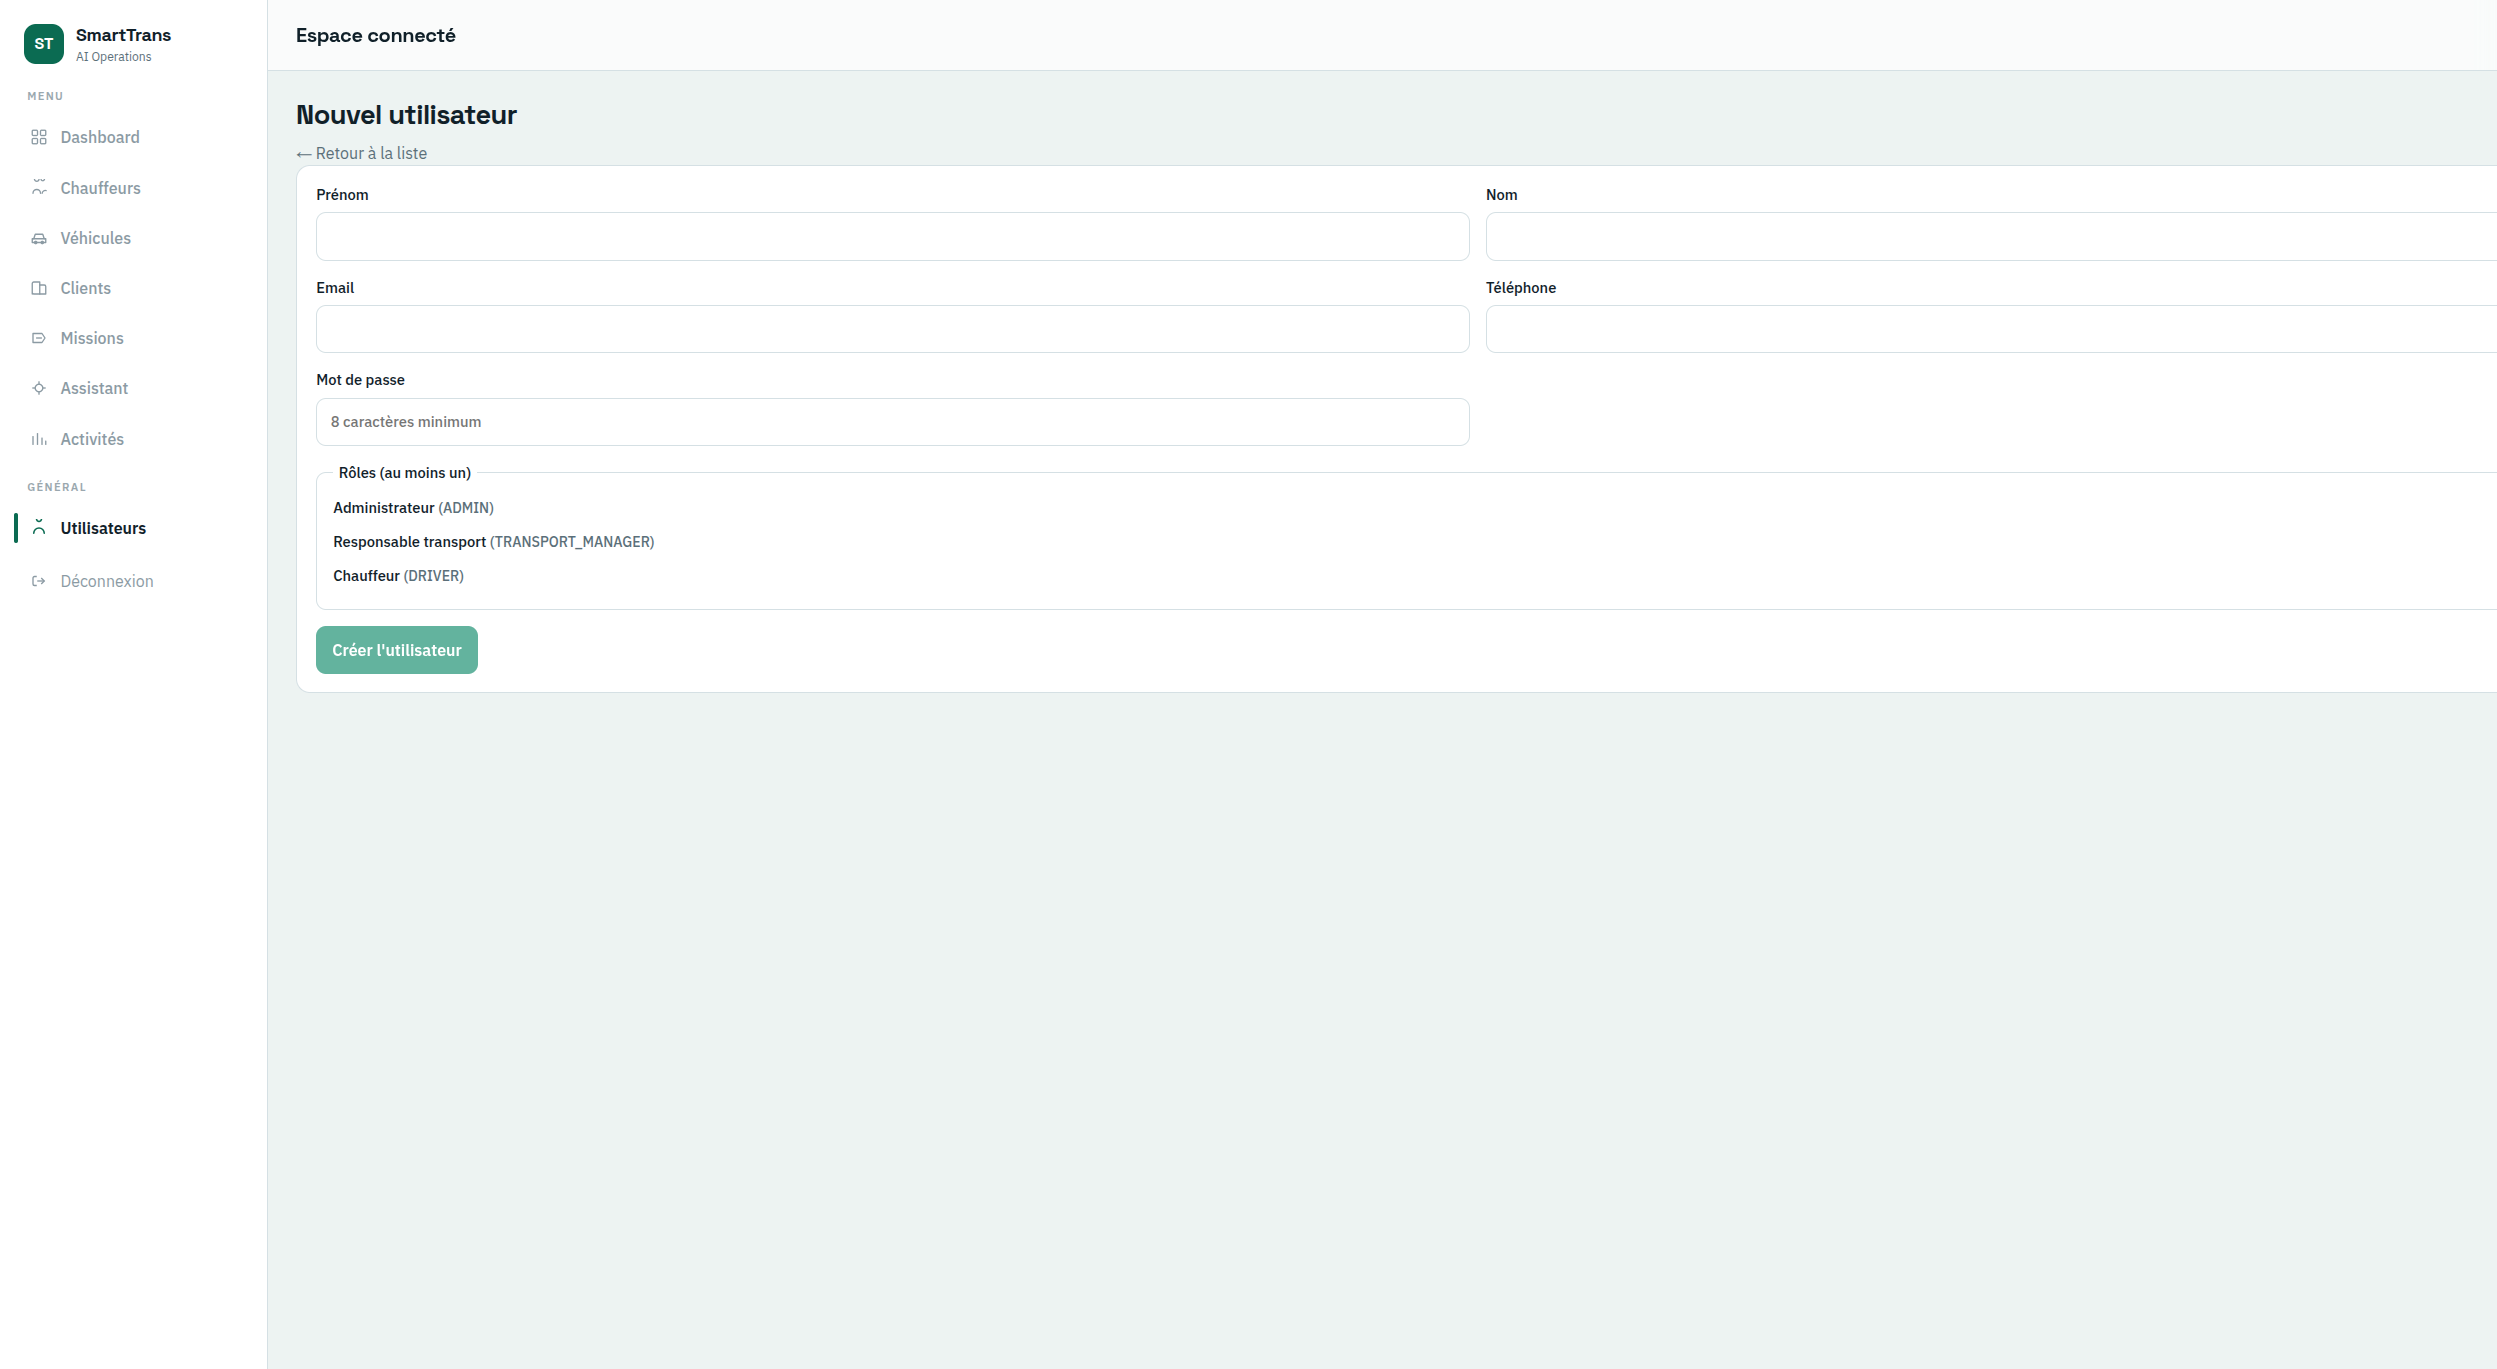
\includegraphics[width=0.88\textwidth,keepaspectratio]{ui-20-utilisateur-nouveau.png}
\caption{Formulaire de création d'un utilisateur}
\label{fig:ui-usr-new}
\end{figure}

\begin{figure}[htbp]
\centering
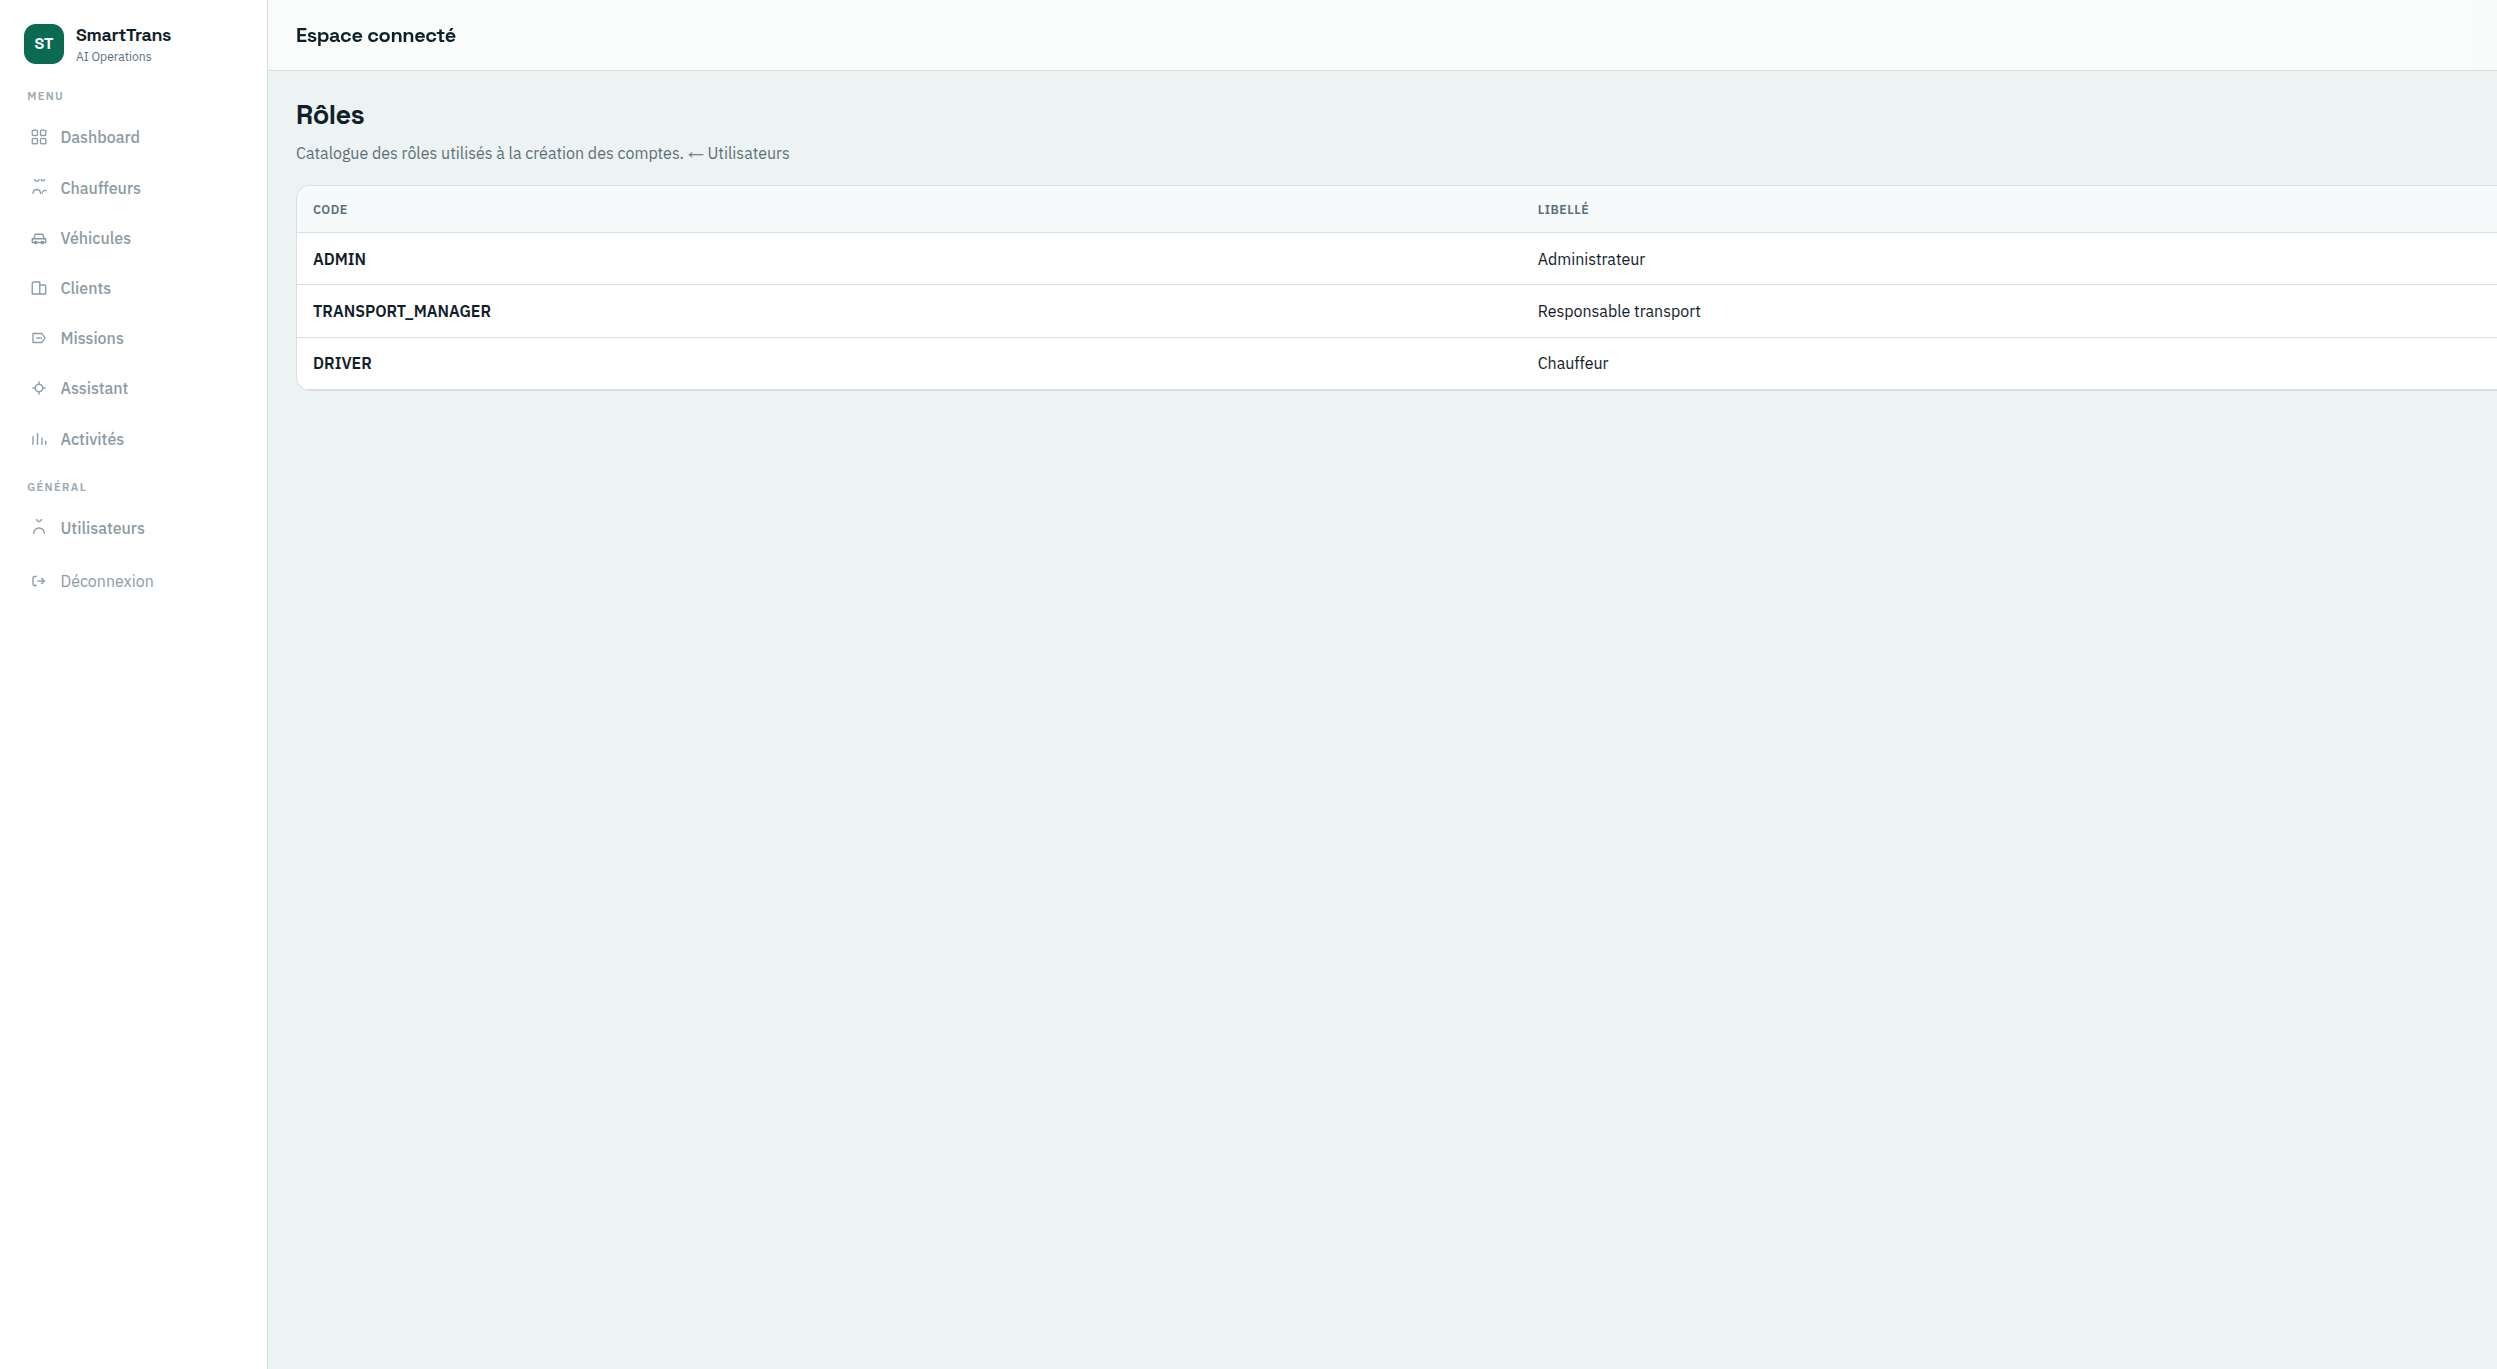
\includegraphics[width=0.88\textwidth,keepaspectratio]{ui-19-roles.png}
\caption{Catalogue des rôles}
\label{fig:ui-rol}
\end{figure}

\section{Conclusion}

Les captures confirment la cohérence de l'interface avec l'analyse : navigation par rôle, formulaires alignés sur le modèle de données, tableau de bord orienté alertes, assistant et journal pour le pilotage. La conclusion générale dresse le bilan du stage.


\chapter*{Conclusion générale et perspectives}
\addcontentsline{toc}{chapter}{Conclusion générale et perspectives}

Le stage a permis de concevoir et d'implémenter \textbf{SmartTrans-AI}, une application de gestion de transport centrée sur la mission, les rôles et un assistant ancré sur les données. Du point de vue pédagogique, le travail a mobilisé l'état de l'art, la spécification UML, la conception d'une API REST sécurisée, une interface selon le profil utilisateur, une première intégration d'IA contrainte par le SI, ainsi que la conduite d'un projet itératif.

Du point de vue de l'organisme, le livrable offre une base opérationnelle pour le département informatique de S. WATRANS : planification, suivi, alertes d'expiration et traçabilité. Les perspectives immédiates concernent le renforcement des tests métier, le déploiement sécurisé, et d'éventuels modules (notifications, pièces jointes, interfaçage temps réel) si le besoin s'en confirme.

Ce rapport, tenu dans une fourchette d'une quarantaine de pages (limite ENSIASD : soixante-dix pages), constitue la trace écrite de cette réalisation.


\begin{thebibliography}{99}
\addcontentsline{toc}{chapter}{Références bibliographiques}

\bibitem{spring}
Spring, Spring Boot Reference Documentation, \url{https://docs.spring.io/spring-boot/} . 29-08-2026.

\bibitem{react}
Meta Open Source, React Documentation, \url{https://react.dev/} . 29-08-2026.

\bibitem{postgres}
PostgreSQL Global Development Group, PostgreSQL Documentation, \url{https://www.postgresql.org/docs/} . 29-08-2026.

\bibitem{uml}
Object Management Group, OMG Unified Modeling Language (OMG UML), Object Management Group, 2017.

\bibitem{jwt}
JONES M., BRADLEY J., SAKIMURA N., JSON Web Token (JWT), RFC 7519, IETF, 2015.

\end{thebibliography}


\appendix
\clearpage
\setcounter{chapter}{1}%
\renewcommand{\thechapter}{A}%
\setcounter{table}{0}%
\setcounter{figure}{0}%
\setcounter{schema}{0}%
\chapter*{Annexe A}
\addcontentsline{toc}{chapter}{Annexe A --- Guide technique de déploiement et d'exécution}

\noindent Cette annexe décrit le guide technique de déploiement et d'exécution de SmartTrans-AI.

\section*{A.1 Backend}

\subsection*{Prérequis}

\begin{itemize}
  \item Java 25 ;
  \item Maven Wrapper fourni dans le dépôt ;
  \item PostgreSQL, via Docker Compose en environnement de développement ou via une instance locale.
\end{itemize}

\subsection*{Lancement}

Depuis le répertoire \texttt{backend} :

\begin{verbatim}
./mvnw spring-boot:run
\end{verbatim}

\subsection*{Vérification de l'état de l'application}

L'état de santé de l'API peut être vérifié à l'adresse :

\url{http://127.0.0.1:8080/actuator/health}

\subsection*{Documentation de l'API}

La documentation OpenAPI/Swagger est accessible à :

\url{http://127.0.0.1:8080/swagger-ui.html}

L'API est accessible sous le préfixe \texttt{/api/v1}.

\subsection*{Compte administrateur de démonstration}

Un compte administrateur est disponible en environnement de développement :

\texttt{admin@smarttrans.ai}

Le mot de passe est défini dans la configuration locale de l'application.

\section*{A.2 Frontend}

Depuis le répertoire \texttt{frontend}, installer les dépendances :

\begin{verbatim}
npm install
\end{verbatim}

Puis lancer l'application :

\begin{verbatim}
npm run dev
\end{verbatim}

L'interface est accessible à l'adresse :

\url{http://127.0.0.1:5173}

Le proxy Vite relaie les requêtes \texttt{/api} vers le backend exécuté sur le port \texttt{8080}.

\section*{A.3 Stack Docker}

Le fichier \texttt{docker-compose.prod.yml} permet d'assembler les principaux services de l'application :

\begin{itemize}
  \item PostgreSQL ;
  \item l'API backend ;
  \item l'interface frontend.
\end{itemize}

Les informations sensibles, notamment les mots de passe et les clés secrètes, doivent être configurées à l'aide d'un fichier d'environnement non versionné.

\clearpage
\setcounter{chapter}{2}%
\renewcommand{\thechapter}{B}%
\setcounter{table}{0}%
\setcounter{figure}{0}%
\setcounter{schema}{0}%
\chapter*{Annexe B}
\addcontentsline{toc}{chapter}{Annexe B --- Documentation de l'API REST}

\noindent Cette annexe documente l'API REST de SmartTrans-AI (préfixe \texttt{/api/v1}). La description interactive est également disponible via OpenAPI/Swagger : \url{http://127.0.0.1:8080/swagger-ui.html}.

\section*{B.1 Conventions}

\begin{itemize}
  \item Format d'échange : JSON (\texttt{Content-Type: application/json}).
  \item Identifiants : UUID.
  \item Authentification : en-tête \texttt{Authorization: Bearer <jeton>}, sauf \texttt{POST /api/v1/auth/login}.
  \item Rôles : \texttt{ADMIN}, \texttt{TRANSPORT\_MANAGER}, \texttt{DRIVER}.
\end{itemize}

\section*{B.2 Authentification}

\begin{table}[htbp]
\centering
\caption{Authentification}
\label{tab:api-auth}
\begin{tabular}{|p{0.38\textwidth}|p{0.14\textwidth}|p{0.38\textwidth}|}
\hline
\TableHead
\tht{Ressource} & \tht{Méthode} & \tht{Description} \\
\hline
\texttt{/api/v1/auth/login} & POST & Connexion ; retourne le JWT et le profil \\
\hline
\end{tabular}
\end{table}

\section*{B.3 Utilisateurs et rôles}

Les ressources suivantes sont réservées à l'administrateur.

\begin{table}[htbp]
\centering
\caption{Utilisateurs et rôles}
\label{tab:api-users}
\begin{tabular}{|p{0.38\textwidth}|p{0.14\textwidth}|p{0.38\textwidth}|}
\hline
\TableHead
\tht{Ressource} & \tht{Méthode} & \tht{Description} \\
\hline
\texttt{/api/v1/users} & GET, POST & Liste et création des comptes \\
\hline
\texttt{/api/v1/users/\{id\}} & GET, PATCH, DELETE & Lecture, mise à jour, suppression \\
\hline
\texttt{/api/v1/roles} & GET, POST & Liste et création des rôles \\
\hline
\texttt{/api/v1/roles/\{id\}} & GET, PATCH, DELETE & Lecture, mise à jour, suppression \\
\hline
\end{tabular}
\end{table}

\section*{B.4 Référentiels métier}

Clients, chauffeurs et véhicules sont gérés par l'administrateur et le responsable transport. Le chauffeur accède à son profil (\texttt{/drivers/me}), à la consultation limitée des fiches et à la mise à jour de sa disponibilité.

\begin{table}[htbp]
\centering
\caption{Clients, chauffeurs et véhicules}
\label{tab:api-ref}
\begin{tabular}{|p{0.44\textwidth}|p{0.14\textwidth}|p{0.32\textwidth}|}
\hline
\TableHead
\tht{Ressource} & \tht{Méthode} & \tht{Description} \\
\hline
\texttt{/api/v1/clients} & GET, POST & Liste et création \\
\hline
\texttt{/api/v1/clients/\{id\}} & GET, PATCH, DELETE & Fiche client \\
\hline
\texttt{/api/v1/drivers} & GET, POST & Liste et création \\
\hline
\texttt{/api/v1/drivers/me} & GET & Profil du chauffeur connecté \\
\hline
\texttt{/api/v1/drivers/expiring-licenses} & GET & Permis proches de l'échéance \\
\hline
\texttt{/api/v1/drivers/\{id\}} & GET, PATCH, DELETE & Fiche chauffeur \\
\hline
\texttt{/api/v1/drivers/\{id\}/availability} & PATCH & Disponibilité \\
\hline
\texttt{/api/v1/drivers/\{id\}/deactivate} & PATCH & Désactivation \\
\hline
\texttt{/api/v1/vehicles} & GET, POST & Liste et création \\
\hline
\texttt{/api/v1/vehicles/expiring-documents} & GET & Assurance / visite technique \\
\hline
\texttt{/api/v1/vehicles/\{id\}} & GET, PATCH, DELETE & Fiche véhicule \\
\hline
\texttt{/api/v1/vehicles/\{id\}/deactivate} & PATCH & Désactivation \\
\hline
\end{tabular}
\end{table}

\section*{B.5 Missions}

Le chauffeur peut consulter les missions qui le concernent et enchaîner les statuts autorisés (planifiée $\rightarrow$ en cours $\rightarrow$ terminée). L'annulation reste du ressort de l'exploitation.

\begin{table}[htbp]
\centering
\caption{Missions}
\label{tab:api-missions}
\begin{tabular}{|p{0.42\textwidth}|p{0.14\textwidth}|p{0.34\textwidth}|}
\hline
\TableHead
\tht{Ressource} & \tht{Méthode} & \tht{Description} \\
\hline
\texttt{/api/v1/missions} & GET, POST & Liste et planification \\
\hline
\texttt{/api/v1/missions/\{id\}} & GET, PATCH, DELETE & Fiche mission \\
\hline
\texttt{/api/v1/missions/\{id\}/status} & PATCH & Changement de statut \\
\hline
\end{tabular}
\end{table}

\section*{B.6 Journal et assistant}

Le journal est en lecture seule. L'assistant est réservé à l'administrateur et au responsable transport.

\begin{table}[htbp]
\centering
\caption{Journal et assistant}
\label{tab:api-pilotage}
\begin{tabular}{|p{0.40\textwidth}|p{0.14\textwidth}|p{0.36\textwidth}|}
\hline
\TableHead
\tht{Ressource} & \tht{Méthode} & \tht{Description} \\
\hline
\texttt{/api/v1/activities} & GET & Journal d'audit \\
\hline
\texttt{/api/v1/activities/\{id\}} & GET & Détail d'un événement \\
\hline
\texttt{/api/v1/assistant/ask} & POST & Question métier ancrée sur les données \\
\hline
\end{tabular}
\end{table}

\section*{B.7 Accès à la documentation interactive}

Avec le backend démarré (\texttt{./mvnw spring-boot:run}), ouvrir :

\url{http://127.0.0.1:8080/swagger-ui.html}

L'état de l'API est indiqué par \url{http://127.0.0.1:8080/actuator/health}.


\end{document}
